\documentclass[
  final,
  babelLanguage=british,
  desktopVersion,
  %showtrims,
  %overleaf,
]{anecdote-reference}

%\graphicspath{{./assets/photos/300dpi/}}
\graphicspath{{./assets/photos/92dpi/}}

% Page size: 210mm x 148mm (A5)
%
% Body text: 12.5 / 18 pt

\usepackage{local}

%% Details of the book
%% ===================

\title{Bhikkhu Manual}
\subtitle{Essential Chants and Vinaya Notes}
\author{Forest Sangha Publications}
\publisher{Forest Sangha Publications}
\date{2019-01-21}% chktex 8
\editionInfo{\textit{Fourth edition}, 2020}
\ISBN{000-000-0000-00-0}% TODO update ISBN % chktex 8

% === Metadata ===

\hypersetup{
  pdftitle={\thetitle},
  pdfauthor={\theauthor},
  pdfcopyright={Copyright (C) 2020, \thePublisher},
  pdfsubject={},% TODO subject
  pdfkeywords={},% TODO keywords
  pdflicenseurl={https://creativecommons.org/licenses/by-nc-nd/4.0/},
  pdfcontacturl={},
  pdflang={en},
}

% FIXME \pdfinfo
%\pdfinfo{%
%  /Title (\thetitle)%
%  /Author (\theauthor)
%  /Subject (subject)% TODO subject
%  /Keywords (keywords)% TODO keywords
%  /GTS_PDFXVersion (PDF/X-1:2001)%
%  /GTS_PDFXConformance (PDF/X-1a:2001)%
%}

%% === Load further packages ===

%% === Hyphenation exceptions and corrections ===

\hyphenation{London}

\openany%

\begin{document}

\frontmatter

\ifdesktopversion
\desktopCover{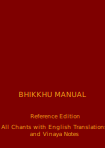
\includegraphics[height=\paperheight]{./reference-cover.png}}
\fi

\cleartorecto
\thispagestyle{empty}
\vspace*{5em}

{\centering

\settowidth{\titleLength}{%
  {\Large\chapterTitleFont\scshape\MakeLowercase{\thetitle}}%
}

{\Large\chapterTitleFont\scshape\MakeLowercase{\thetitle}}\\[0.3\baselineskip]
\setlength{\xheight}{\heightof{X}}
\raisebox{0.5\xheight}{\color[gray]{0.4}\rule{\titleLength}{0.25pt}}\\[0.3\baselineskip]
{\itshape
\thesubtitle}

\vfill

\theauthor

\vspace*{5em}

}



\cleartoverso
\thispagestyle{empty}

\vspace*{-\baselineskip}

{%

\ifhandbookedition
\fontsize{9}{10}\selectfont
\else
\fontsize{9}{11}\selectfont
\fi
\centering
\setlength{\parindent}{0pt}%
\setlength{\parskip}{0.8\baselineskip}%

\thetitle\\
\thesubtitle\\
\ifhandbookedition
Handbook Edition
\else
Reference Edition
\fi

Published by Amaravati Publications

ISBN \theISBN

Copyright \copyright\ Amaravati Buddhist Monastery 2020

This book is offered for free distribution,\\
please do not sell this book.

Download this book in PDF, EPUB and MOBI formats\\
at the following addresses:

\href{https://forestsangha.org/}{www.forestsangha.org}

\href{https://www.amaravati.org/}{www.amaravati.org}

\href{https://bhikkhu-manual.github.io/}{bhikkhu-manual.github.io}

\vfill

This work is licensed under a Creative Commons\\
Attribution-NonCommercial-NoDerivatives 4.0 International~License.

Produced with the \LaTeX\ typesetting system,\\
set in Gentium and Nunito~Sans.

\theEditionInfo

}


\cleartorecto
\thispagestyle{empty}

\mbox{}\vfill

\begin{verse}

{\itshape
Lorem ipsum dolor sit amet,\\
consectetuer adipiscing elit.
}


\end{verse}

\vfill\mbox{}


\clearpage
{\subsectionFmt{Abbreviations used in the text}}
\bigskip

% FIXME: reformat references to accord with this
% Gavesako: References to shorter texts consisting of verses such as the Dhammapada, Udāna, Itivuttaka, Theragāthā, Therīgāthā or Sutta Nipāta are to the verse number or chapter and verse number. The other longer texts are referred to by volume and page number of the PTS edition.

% Gavesako: Add:  Sp  Samantapāsādikā
%                 Kv  Kaṅkhāvitaraṇī 
                 

\bigskip

\begin{tabular}{@{}ll ll@{}}
  A & Aṅguttara Nikāya & Pr & Pārājika\\
  Cv & Cullavagga &       Pv & Parivāra\\
  Dhp & Dhammapada &      S & Saṃyutta Nikāya \\
  D & Dīgha Nikāya  &    Snp & Sutta Nipāta\\
  It & Itivuttaka &       Th & Theragāthā \\
  Ja & Jātaka &           Thī & Therīgāthā\\
  Khp & Khuddakapāṭha &   Ud & Udāna\\
  M & Majjhima Nikāya &  Vin & Vinaya Piṭaka\\
  Mv & Mahāvagga &        DhpA & Dhammapada Aṭṭhakathā\\
  &                    &  Vism & Visuddhimagga\\
\end{tabular}

% \bigskip
%
% {\subsectionFmt{Looking up references}}
% \bigskip
%
% TODO: Add instructions on how to look up references.



\cleartorecto
\pagestyle{toponerow-frontmatter}
\tableofcontents*

\clearpage
\listfirstlines*

\input{./manuscript/tex/preface.tex}

\mainmatter
\pagestyle{toponerow}

\cleartorecto
\part{Essential Chants}

{\raggedright

\chapter{Morning Chanting}

\section*{Dedication of Offerings}

[Yo so] bhagavā arahaṁ sammāsambuddho\\
Svākkhāto yena bhagavatā dhammo\\
Supaṭipanno yassa bhagavato sāvakasaṅgho\\
Tam-mayaṁ bhagavantaṁ sadhammaṁ sasaṅghaṁ\\
Imehi sakkārehi yathārahaṁ āropitehi abhipūjayāma\\
Sādhu no bhante bhagavā sucira-parinibbutopi\\
Pacchimā-janatānukampa-mānasā\\
Ime sakkāre duggata-paṇṇākāra-bhūte paṭiggaṇhātu\\
Amhākaṁ dīgharattaṁ hitāya sukhāya\\
Arahaṁ sammāsambuddho bhagavā\\
Buddhaṁ bhagavantaṁ abhivādemi\\\relax
[Svākkhāto] bhagavatā dhammo\\
Dhammaṁ namassāmi\\\relax
[Supaṭipanno] bhagavato sāvakasaṅgho\\
Saṅghaṁ namāmi

\section*{Dedication of Offerings (English)}

To the Blessed One, the Lord,\\\vin who fully attained perfect enlightenment,\\
To the Teaching which he expounded so well,\\
And to the Blessed One's disciples who have practised well,\\
To these --- the Buddha, the Dhamma, and the Saṅgha ---\\
We render with offerings our rightful homage.\\
It is well for us that the Blessed One, having attained liberation,\\
Still had compassion for later generations.\\
May these simple offerings be accepted\\
For our long-lasting benefit and for the happiness it gives us.

The Lord, the Perfectly Enlightened and Blessed One ---\\
I render homage to the Buddha, the Blessed One.

The Teaching so completely explained by him ---\\
I bow to the Dhamma.

The Blessed One's disciples who have practised well ---\\
I bow to the Saṅgha.

\section*{Preliminary Homage}

\begin{leader}
  [Handa mayaṁ buddhassa bhagavato pubbabhāga-namakāraṁ karomase]
\end{leader}

Namo tassa bhagavato arahato sammāsambuddhassa (×3)

\section*{Preliminary Homage (English)}

\begin{leader}
  [Now let us pay preliminary homage to the Buddha.]
\end{leader}

Homage to the Blessed, Noble, and Perfectly Enlightened One. (×3)

\clearpage

\section*{Homage to the Buddha}

\begin{leader}
  [Handa mayaṁ buddhābhitthutiṁ karomase]
\end{leader}

Yo so tathāgato arahaṁ sammāsambuddho\\
Vijjācaraṇa-sampanno sugato lokavidū\\
Anuttaro purisadamma-sārathi\\
Satthā deva-manussānaṁ buddho bhagavā

Yo imaṁ lokaṁ sadevakaṁ samārakaṁ sabrahmakaṁ\\
Sassamaṇa-brāhmaṇiṁ pajaṁ sadeva-manussaṁ sayaṁ abhiññā sacchikatvā pavedesi\\
Yo dhammaṁ desesi ādi-kalyāṇaṁ majjhe-kalyāṇaṁ pariyosāna-kalyāṇaṁ\\
Sātthaṁ sabyañjanaṁ kevala-paripuṇṇaṁ parisuddhaṁ brahma-cariyaṁ pakāsesi\\
Tam-ahaṁ bhagavantaṁ abhipūjayāmi\\
Tam-ahaṁ bhagavantaṁ sirasā namāmi

\section*{Homage to the Buddha (English)}

\begin{leader}
  [Now let us chant in praise of the Buddha.]
\end{leader}

The Tathāgata is the Pure One, the Perfectly Enlightened One.\\
He is impeccable in conduct and understanding,\\
The Accomplished One,\\
The Knower of the Worlds.\\
He trains perfectly those who wish to be trained.\\
He is Teacher of gods and humans.\\
He is awake and holy.\\
In this world with its gods, demons, and kind spirits,\\
Its seekers and sages, celestial and human beings, he has by \\deep insight revealed the Truth.\\
He has pointed out the Dhamma: beautiful in the beginning, \\beautiful in the middle, beautiful in the end.\\
He has explained the Spiritual Life of complete purity in its \\essence and conventions.\\
I chant my praise to the Blessed One, I bow my head to \\the Blessed One.

\section*{Homage to the Dhamma}

\begin{leader}
  [Handa mayaṁ dhammābhitthutiṁ karomase]
\end{leader}

Yo so svākkhāto bhagavatā dhammo\\
Sandiṭṭhiko akāliko ehipassiko opanayiko\\
Paccattaṁ veditabbo viññūhi\\
Tam-ahaṁ dhammaṁ abhipūjayāmi\\
Tam-ahaṁ dhammaṁ sirasā namāmi

\section*{Homage to the Dhamma (English)}

\begin{leader}
  [Now let us chant in praise of the Dhamma.]
\end{leader}

The Dhamma is well expounded by the Blessed One,\\
Apparent here and now,\\
Timeless,\\
Encouraging investigation,\\
Leading inwards,\\
To be experienced individually by the wise.\\
I chant my praise to this Teaching, I bow my head\\ to this Truth.

\section*{Homage to the Saṅgha}

\begin{leader}
  [Handa mayaṁ saṅghābhitthutiṁ karomase]
\end{leader}

Yo so supaṭipanno bhagavato sāvakasaṅgho\\
Ujupaṭipanno bhagavato sāvakasaṅgho\\
Ñāyapaṭipanno bhagavato sāvakasaṅgho\\
Sāmīcipaṭipanno bhagavato sāvakasaṅgho\\
Yadidaṁ cattāri purisayugāni aṭṭha purisapuggalā\\
Esa bhagavato sāvakasaṅgho\\
Āhuneyyo pāhuneyyo dakkhiṇeyyo añjali-karaṇīyo\\
Anuttaraṁ puññakkhettaṁ lokassa\\
Tam-ahaṁ saṅghaṁ abhipūjayāmi\\
Tam-ahaṁ saṅghaṁ sirasā namāmi

\section*{Homage to the Saṅgha (English)}

\begin{leader}
  [Now let us chant in praise of the Saṅgha.]
\end{leader}

They are the Blessed One's disciples, who have practised well,\\
Who have practised directly,\\
Who have practised insightfully,\\
Those who practise with integrity ---\\
That is the four pairs, the eight kinds of noble beings ---\\
These are the Blessed One's disciples.\\
Such ones are worthy of gifts,\\
Worthy of hospitality,\\
Worthy of offerings,\\
Worthy of respect;\\
They give occasion for incomparable goodness to arise \\in the world.\\
I chant my praise to this Saṅgha, I bow my head to\\ this Saṅgha.

\section*{Salutation to the Triple Gem}

\begin{leader}
  [Handa mayaṁ ratanattaya-paṇāma-gāthāyo c'eva\\
  saṁvega-parikittana-pāṭhañca bhaṇāmase]
\end{leader}

\firstline{Buddho susuddho karuṇā-mahaṇṇavo}

Buddho susuddho karuṇā-mahaṇṇavo\\
Yo'ccanta-suddhabbara-ñāṇa-locano\\
Lokassa pāpūpakilesa-ghātako\\
Vandāmi buddhaṁ aham-ādarena taṁ\\
Dhammo padīpo viya tassa satthuno\\
Yo magga-pākāmata-bheda-bhinnako\\
Lokuttaro yo ca tad-attha-dīpano\\
Vandāmi dhammaṁ aham-ādarena taṁ\\
Saṅgho sukhettābhyati-khetta-saññito\\
Yo diṭṭha-santo sugatānubodhako\\
Lolappahīno ariyo sumedhaso\\
Vandāmi saṅghaṁ aham-ādarena taṁ\\
Iccevam-ekantabhipūja-neyyakaṁ vatthuttayaṁ \\vandayatābhisaṅkhataṁ\\
Puññaṁ mayā yaṁ mama sabbupaddavā mā hontu ve tassa pabhāva-siddhiyā

Idha tathāgato loke uppanno arahaṁ sammāsambuddho\\
Dhammo ca desito niyyāniko upasamiko parinibbāniko sambodhagāmī sugatappavedito\\
Mayan-taṁ dhammaṁ sutvā evaṁ jānāma

Jātipi dukkhā\\
Jarāpi dukkhā\\
Maraṇampi dukkhaṁ\\
Soka-parideva-dukkha-domanass'upāyāsāpi dukkhā\\
Appiyehi sampayogo dukkho\\
Piyehi vippayogo dukkho\\
Yamp'icchaṁ na labhati tampi dukkhaṁ\\
Saṅkhittena pañcupādānakkhandhā dukkhā

Seyyathīdaṁ\\
Rūpūpādānakkhandho\\
Vedanūpādānakkhandho\\
Saññūpādānakkhandho\\
Saṅkhārūpādānakkhandho\\
Viññāṇūpādānakkhandho

Yesaṁ pariññāya\\
Dharamāno so bhagavā evaṁ bahulaṁ sāvake vineti\\
Evaṁ bhāgā ca panassa bhagavato sāvakesu anusāsanī bahulā pavattati

Rūpaṁ aniccaṁ\\
Vedanā aniccā\\
Saññā aniccā\\
Saṅkhārā aniccā\\
Viññāṇaṁ aniccaṁ\\
Rūpaṁ anattā\\
Vedanā anattā\\
Saññā anattā\\
Saṅkhārā anattā\\
Viññāṇaṁ anattā\\
Sabbe saṅkhārā aniccā\\
Sabbe dhammā anattā'ti

Te mayaṁ otiṇṇāmha jātiyā jarā-maraṇena\\
Sokehi paridevehi dukkhehi domanassehi upāyāsehi\\
Dukkhotiṇṇā dukkha-paretā\\
Appeva nāmimassa kevalassa dukkha-kkhandhassa\\
antakiriyā paññāyethā'ti

Cira-parinibbutampi taṁ bhagavantaṁ uddissa arahantaṁ sammāsambuddhaṁ\\
Saddhā agārasmā anagāriyaṁ pabbajitā\\
Tasmiṁ bhagavati brahma-cariyaṁ carāma\\
Bhikkhūnaṁ/Sīladharānaṁ sikkhāsājīva-samāpannā\\
Taṁ no brahma-cariyaṁ imassa kevalassa dukkha-kkhandhassa antakiriyāya saṁvattatu

\section*{Salutation to the Triple Gem (English)}

\begin{leader}
  [Now let us chant our salutation to the Triple Gem and a passage to arouse urgency.]
\end{leader}

The Buddha, absolutely pure, with ocean-like compassion,\\
Possessing the clear sight of wisdom,\\
Destroyer of worldly self-corruption ---\\
Devotedly indeed, that Buddha I revere.\\
The Teaching of the Lord, like a lamp,\\
Illuminating the Path and its Fruit: the Deathless,\\
That which is beyond the conditioned world ---\\
Devotedly indeed, that Dhamma I revere.\\
The Saṅgha, the most fertile ground for cultivation,\\
Those who have realized peace, awakened after the \\Accomplished One,\\
Noble and wise, all longing abandoned ---\\
Devotedly indeed, that Saṅgha I revere.

This salutation should be made to that which is worthy.\\
Through the power of such good action,\\\vin may all obstacles disappear.\\
One who knows things as they are has come into this world; and he is an Arahant, a perfectly Awakened being,\\
Purifying the way leading out of delusion, calming and directing to perfect peace, and leading to enlightenment --- this Way he has made known.

Having heard the Teaching, we know this:\\
Birth is dukkha,\\
Ageing is dukkha,\\
And death is dukkha;\\
Sorrow, lamentation, pain, grief, and despair are dukkha;\\
Association with the disliked is dukkha;\\
Separation from the liked is dukkha;\\
Not attaining one's wishes is dukkha.\\
In brief, the five focuses of identity are dukkha.

These are as follows:\\
Attachment to form,\\
Attachment to feeling,\\
Attachment to perception,\\
Attachment to mental formations,\\
Attachment to sense-consciousness.\\
For the complete understanding of this,\\
The Blessed One in his lifetime frequently instructed his disciples \\in just this way.

In addition, he further instructed:\\
Form is impermanent,\\
Feeling is impermanent,\\
Perception is impermanent,\\
Mental formations are impermanent,\\
Sense-consciousness is impermanent;

Form is not-self,\\
Feeling is not-self,\\
Perception is not-self,\\
Mental formations are not-self,\\
Sense-consciousness is not-self;\\
All conditions are transient,\\
There is no self in the created or the uncreated.\\
All of us are bound by birth, ageing, and death,\\
By sorrow, lamentation, pain, grief, and despair,\\
Bound by dukkha and obstructed by dukkha.\\
Let us all aspire to complete freedom from suffering.

\begin{instruction}
  The following is chanted only by the monks and nuns.
\end{instruction}

Remembering the Blessed One, the Noble Lord, and Perfectly Enlightened One, who long ago attained Parinibbāna,\\
We have gone forth with faith from home to homelessness,\\
And like the Blessed One, we practise the Holy Life,\\
Being fully equipped with the bhikkhus'/nuns' system of training.\\
May this Holy Life lead us to the end of this whole mass\\ of suffering.\\

\begin{instruction}
  An alternative version of the preceding section, which can be chanted by laypeople as well.
\end{instruction}

The Blessed One, who long ago attained Parinibbāna, is our refuge.\\
So too are the Dhamma and the Saṅgha.\\
Attentively we follow the pathway of that Blessed One, with all of \\our mindfulness and strength.\\
May then the cultivation of this practice\\
Lead us to the end of every kind of suffering.

\section*{Closing Homage}

[Arahaṁ] sammāsambuddho bhagavā\\
Buddhaṁ bhagavantaṁ abhivādemi

[Svākkhāto] bhagavatā dhammo\\
Dhammaṁ namassāmi

[Supaṭipanno] bhagavato sāvakasaṅgho\\
Saṅghaṁ namāmi

\section*{Closing Homage (English)}

The Lord, the Perfectly Enlightened and Blessed One ---\\
I render homage to the Buddha, the Blessed One.

The Teaching, so completely explained by him ---\\
I bow to the Dhamma.

The Blessed One's disciples, who have practised well ---\\
I bow to the Saṅgha.


\chapter{Evening Chanting}

\section*{Dedication of Offerings}

\firstline{Yo so bhagavā arahaṁ sammāsambuddho}

[Yo so] bhagavā arahaṁ sammāsambuddho\\
Svākkhāto yena bhagavatā dhammo\\
Supaṭipanno yassa bhagavato sāvakasaṅgho\\
Tam-mayaṁ bhagavantaṁ sadhammaṁ sasaṅghaṁ\\
Imehi sakkārehi yathārahaṁ āropitehi abhipūjayāma\\
Sādhu no bhante bhagavā sucira-parinibbutopi\\
Pacchimā-janatānukampa-mānasā\\
Ime sakkāre duggata-paṇṇākāra-bhūte paṭiggaṇhātu\\
Amhākaṁ dīgharattaṁ hitāya sukhāya\\
Arahaṁ sammāsambuddho bhagavā\\
Buddhaṁ bhagavantaṁ abhivādemi

[Svākkhāto] bhagavatā dhammo\\
Dhammaṁ namassāmi

[Supaṭipanno] bhagavato sāvakasaṅgho\\
Saṅghaṁ namāmi

\section*{Dedication of Offerings (English)}

[To the Blessed One,] the Lord, who fully attained\\
\vin perfect enlightenment,\\
To the Teaching, which he expounded so well,\\
And to the Blessed One's disciples who have practised well,\\
To these --- the Buddha, the Dhamma, and the Saṅgha ---\\
We render with offerings our rightful homage.\\
It is well for us that the Blessed One, having attained liberation,\\
Still had compassion for later generations.\\
May these simple offerings be accepted\\
For our long-lasting benefit and for the happiness it gives us.\\
The Lord, the Perfectly Enlightened and Blessed One ---\\
I render homage to the Buddha, the Blessed One.

[The Teaching,] so completely explained by him ---\\
I bow to the Dhamma.

[The Blessed One's disciples,] who have practised well ---\\
I bow to the Saṅgha.

\section*{Preliminary Homage}

\begin{leader}
  [Handa mayaṁ buddhassa bhagavato pubbabhāga-namakāraṁ karomase]
\end{leader}

Namo tassa bhagavato arahato sammāsambuddhassa (×3)

\section*{Preliminary Homage (English)}

\begin{leader}
  [Now let us pay preliminary homage to the Buddha.]
\end{leader}

Homage to the Blessed, Noble, and Perfectly Enlightened One. (×3)

\clearpage

\section*{Recollection of the Buddha}

\begin{leader}
  [Handa mayaṁ buddhānussatinayaṁ karomase]
\end{leader}

Taṁ kho pana bhagavantaṁ evaṁ kalyāṇo\\
\vin kittisaddo abbhuggato\\
Itipi so bhagavā arahaṁ sammāsambuddho\\
Vijjācaraṇa-sampanno sugato lokavidū\\
Anuttaro purisadamma-sārathi satthā deva-manussānaṁ\\
\vin buddho bhagavā'ti

\section*{Recollection of the Buddha (English)}

\begin{leader}
  [Now let us chant the recollection of the Buddha.]
\end{leader}

A good word of the Blessed One's reputation has spread as follows:\\
He, the Blessed One, is indeed the Pure One,\\
\vin the Perfectly Enlightened One;\\
He is impeccable in conduct and understanding,\\
\vin the Accomplished One, the Knower of the Worlds;\\
He trains perfectly those who wish to be trained;\\
\vin he is Teacher of gods and humans; he is Awake and Holy.

\section*{Supreme Praise of the Buddha}

\begin{leader}
  [Handa mayaṁ buddhābhigītiṁ karomase]
\end{leader}

Buddh'vārahanta-varatādiguṇābhiyutto\\
Suddhābhiñāṇa-karuṇāhi samāgatatto\\
Bodhesi yo sujanataṁ kamalaṁ va sūro\\
Vandām'ahaṁ tam-araṇaṁ sirasā jinendaṁ\\
Buddho yo sabba-pāṇīnaṁ saraṇaṁ khemam-uttamaṁ\\
Paṭhamānussatiṭṭhānaṁ vandāmi taṁ siren'ahaṁ\\
Buddhassāh'asmi dāso/dāsī va buddho me sāmi-kissaro\\
Buddho dukkhassa ghātā ca vidhātā ca hitassa me\\
Buddhass'āhaṁ niyyādemi sarīrañ-jīvitañ-cidaṁ\\
Vandanto'haṁ/Vandantī'haṁ carissāmi\\
\vin buddhass'eva subodhitaṁ\\
Natthi me saraṇaṁ aññaṁ buddho me saraṇaṁ varaṁ\\
Etena sacca-vajjena vaḍḍheyyaṁ satthu-sāsane\\
Buddhaṁ me vandamānena/vandamānāya\\
\vin yaṁ puññaṁ pasutaṁ idha\\
Sabbepi antarāyā me māhesuṁ tassa tejasā

\instr{(Bowing)}

Kāyena vācāya va cetasā vā\\
Buddhe kukammaṁ pakataṁ mayā yaṁ\\
Buddho paṭiggaṇhātu accayantaṁ\\
Kālantare saṁvarituṁ va buddhe

\section*{Supreme Praise of the Buddha (English)}

\begin{leader}
  [Now let us chant the supreme praise of the Buddha.]
\end{leader}

The Buddha, the truly worthy one, endowed with\\
\vin such excellent qualities,\\
Whose being is composed of purity, transcendental wisdom,\\
\vin and compassion,\\
Who has enlightened the wise like the sun awakening the lotus ---\\
I bow my head to that peaceful chief of conquerors.\\
The Buddha, who is the safe, secure refuge of all beings ---\\
As the First Object of Recollection,\\\vin I venerate him with bowed head.\\
I am indeed the Buddha's servant,\\\vin the Buddha is my Lord and Guide.\\
The Buddha is sorrow's destroyer, who bestows blessings on me.\\
To the Buddha I dedicate this body and life,\\
And in devotion I will walk the Buddha's Path of Awakening.\\
For me there is no other refuge, the Buddha is my excellent refuge.\\
By the utterance of this Truth, may I grow in the Master's Way.\\
By my devotion to the Buddha, and the blessing of this practice ---\\
By its power, may all obstacles be overcome.

\instr{(Bowing)}

By body, speech, or mind,\\
For whatever wrong action I have committed towards the Buddha,\\
May my acknowledgement of fault be accepted,\\
That in future there may be restraint regarding the Buddha.

\section*{Recollection of the Dhamma}

\begin{leader}
  [Handa mayaṁ dhammānussatinayaṁ karomase]
\end{leader}

Svākkhāto bhagavatā dhammo\\
Sandiṭṭhiko akāliko ehipassiko\\
Opanayiko paccattaṁ veditabbo viññūhī'ti

\clearpage

\section*{Recollection of the Dhamma (English)}

\begin{leader}
  [Now let us chant the recollection of the Dhamma.]
\end{leader}

The Dhamma is well expounded by the Blessed One,\\
Apparent here and now, timeless, encouraging investigation,\\
Leading inwards, to be experienced individually by the wise.

\section*{Supreme Praise of the Dhamma}

\begin{leader}
  [Handa mayaṁ dhammābhigītiṁ karomase]
\end{leader}

Svākkhātat'ādiguṇa-yoga-vasena seyyo\\
Yo magga-pāka-pariyatti-vimokkha-bhedo\\
Dhammo kuloka-patanā tada-dhāri-dhārī\\
Vandām'ahaṁ tama-haraṁ vara-dhammam-etaṁ\\
Dhammo yo sabba-pāṇīnaṁ saraṇaṁ khemam-uttamaṁ\\
Dutiyānussatiṭṭhānaṁ vandāmi taṁ siren'ahaṁ\\
Dhammassāh'asmi dāso/dāsī va dhammo me sāmi-kissaro\\
Dhammo dukkhassa ghātā ca vidhātā ca hitassa me\\
Dhammass'āhaṁ niyyādemi sarīrañ-jīvitañ-cidaṁ\\
Vandantohaṁ/Vandantīhaṁ carissāmi\\
\vin dhammass'eva sudhammataṁ\\
Natthi me saraṇaṁ aññaṁ dhammo me saraṇaṁ varaṁ\\
Etena sacca-vajjena vaḍḍheyyaṁ satthu-sāsane\\
Dhammaṁ me vandamānena/vandamānāya\\
\vin yaṁ puññaṁ pasutaṁ idha\\
Sabbepi antarāyā me māhesuṁ tassa tejasā

\clearpage

\instr{(Bowing)}

Kāyena vācāya va cetasā vā\\
Dhamme kukammaṁ pakataṁ mayā yaṁ\\
Dhammo paṭiggaṇhātu accayantaṁ\\
Kālantare saṁvarituṁ va dhamme

\section*{Supreme Praise of the Dhamma (English)}

\begin{leader}
  [Now let us chant the supreme praise of the Dhamma.]
\end{leader}

It is excellent because it is `well expounded,'\\
And it can be divided into Path and Fruit, Learning and Liberation.\\
The Dhamma holds those who uphold it from falling into delusion.\\
I revere the excellent Teaching, that which removes darkness ---\\
The Dhamma, which is the supreme, secure refuge of all beings ---\\
As the Second Object of Recollection,\\\vin I venerate it with bowed head.\\
I am indeed the Dhamma's servant,\\\vin the Dhamma is my Lord and Guide.\\
The Dhamma is sorrow's destroyer, and it bestows blessings on me.\\
To the Dhamma I dedicate this body and life,\\
And in devotion I will walk this excellent way of Truth.\\
For me there is no other refuge,\\\vin the Dhamma is my excellent refuge.\\
By the utterance of this Truth, may I grow in the Master's Way.\\
By my devotion to the Dhamma, and the blessing of this practice ---\\
By its power, may all obstacles be overcome.

\clearpage

\instr{(Bowing)}

By body, speech, or mind,\\
For whatever wrong action I have committed\\\vin towards the Dhamma,\\
May my acknowledgement of fault be accepted,\\
That in future there may be restraint regarding the Dhamma.

\section*{Recollection of the Saṅgha}

\begin{leader}
  [Handa mayaṁ saṅghānussatinayaṁ karomase]
\end{leader}

Supaṭipanno bhagavato sāvakasaṅgho\\
Ujupaṭipanno bhagavato sāvakasaṅgho\\
Ñāyapaṭipanno bhagavato sāvakasaṅgho\\
Sāmīcipaṭipanno bhagavato sāvakasaṅgho\\
Yadidaṁ cattāri purisayugāni aṭṭha purisapuggalā\\
Esa bhagavato sāvakasaṅgho\\
Āhuneyyo pāhuneyyo dakkhiṇeyyo añjali-karaṇīyo\\
Anuttaraṁ puññakkhettaṁ lokassā'ti

\section*{Recollection of the Saṅgha (English)}

\begin{leader}
  [Now let us chant the recollection of the Saṅgha.]
\end{leader}

They are the Blessed One's disciples, who have practised well,\\
Who have practised directly,\\
Who have practised insightfully,\\
Those who practise with integrity ---\\
That is the four pairs, the eight kinds of noble beings ---\\
These are the Blessed One's disciples.\\
Such ones are worthy of gifts, worthy of hospitality,\\
\vin worthy of offerings, worthy of respect;\\
They give occasion for incomparable goodness\\\vin to arise in the world.

\section*{Supreme Praise of the Saṅgha}

\begin{leader}
  [Handa mayaṁ saṅghābhigītiṁ karomase]
\end{leader}

Saddhammajo supaṭipatti-guṇādiyutto\\
Yo'ṭṭhabbidho ariyapuggala-saṅgha-seṭṭho\\
Sīlādidhamma-pavarāsaya-kāya-citto\\
Vandām'ahaṁ tam-ariyāna-gaṇaṁ susuddhaṁ\\
Saṅgho yo sabba-pāṇīnaṁ saraṇaṁ khemam-uttamaṁ\\
Tatiyānussatiṭṭhānaṁ vandāmi taṁ siren'ahaṁ\\
Saṅghass'āhasmi dāso/dāsī va saṅgho me sāmi-kissaro\\
Saṅgho dukkhassa ghātā ca vidhātā ca hitassa me\\
Saṅghass'āhaṁ niyyādemi sarīrañ-jīvitañ-cidaṁ\\
Vandanto'haṁ/Vandantī'haṁ carissāmi\\
\vin saṅghassopaṭipannataṁ\\
Natthi me saraṇaṁ aññaṁ saṅgho me saraṇaṁ varaṁ\\
Etena sacca-vajjena vaḍḍheyyaṁ satthu-sāsane\\
Saṅghaṁ me vandamānena/vandamānāya\\
\vin yaṁ puññaṁ pasutaṁ idha\\
Sabbepi antarāyā me māhesuṁ tassa tejasā

\instr{(Bowing)}

Kāyena vācāya va cetasā vā\\
Saṅghe kukammaṁ pakataṁ mayā yaṁ\\
Saṅgho paṭiggaṇhātu accayantaṁ\\
Kālantare saṁvarituṁ va saṅghe

\section*{Supreme Praise of the Saṅgha (English)}

\begin{leader}
  [Now let us chant the supreme praise of the Saṅgha.]
\end{leader}

Born of the Dhamma, that Saṅgha which has practised well,\\
The field of the Saṅgha formed of eight kinds of noble beings,\\
Guided in body and mind by excellent morality and virtue.\\
I revere that assembly of noble beings perfected in purity.\\
The Saṅgha, which is the supreme, secure refuge of all beings ---\\
As the Third Object of Recollection, I venerate it with bowed head.

I am indeed the Saṅgha's servant, the Saṅgha is my Lord and Guide.\\
The Saṅgha is sorrow's destroyer and it bestows blessings on me.\\
To the Saṅgha I dedicate this body and life,\\
And in devotion I will walk the well-practised way of the Saṅgha.\\
For me there is no other refuge, the Saṅgha is my excellent refuge.\\
By the utterance of this Truth, may I grow in the Master's Way.\\
By my devotion to the Saṅgha, and the blessing of this practice ---\\
By its power, may all obstacles be overcome.

\instr{(Bowing)}

By body, speech, or mind,\\
For whatever wrong action I have committed towards the Saṅgha,\\
May my acknowledgement of fault be accepted,\\
That in future there may be restraint regarding the Saṅgha.

\section*{Closing Homage}

[Arahaṁ] sammāsambuddho bhagavā\\
Buddhaṁ bhagavantaṁ abhivādemi

[Svākkhāto] bhagavatā dhammo\\
Dhammaṁ namassāmi

[Supaṭipanno] bhagavato sāvakasaṅgho\\
Saṅghaṁ namāmi

\section*{Closing Homage (English)}

[The Lord,] the Perfectly Enlightened and Blessed One ---\\
I render homage to the Buddha, the Blessed One.

[The Teaching,] so completely explained by him ---\\
I bow to the Dhamma.

[The Blessed One's disciples,] who have practised well ---\\
I bow to the Saṅgha.


\chapter{Reflections}

\section{Reflection on the Four Requisites}

\begin{leader}
  [Handa mayaṁ taṅkhaṇika-\\ paccavekkhaṇa-pāṭhaṁ bhaṇāmase]
\end{leader}

\firstline{Paṭisaṅkhā yoniso cīvaraṁ paṭisevāmi}

[Paṭisaṅkhā] yoniso cīvaraṁ paṭisevāmi,\\
yāvadeva sītassa paṭighātāya, uṇhassa paṭighātāya,\\
ḍaṁsa-makasa-vātātapa-siriṁsapa-samphassānaṁ\\
paṭighātāya, yāvadeva hirikopina-paṭicchādanatthaṁ

\begin{english}
  Wisely reflecting, I use the robe: only to ward off cold, to ward off heat, to
  ward off the touch of flies, mosquitoes, wind, burning and creeping things,
  only for the sake of modesty.
\end{english}

[Paṭisaṅkhā] yoniso piṇḍapātaṁ paṭisevāmi, neva davāya, na madāya, na maṇḍanāya,
na vibhūsanāya, yāvadeva imassa kāyassa ṭhitiyā, yāpanāya, vihiṁsūparatiyā,
brahmacariyānuggahāya, iti purāṇañca vedanaṁ paṭihaṅkhāmi, navañca vedanaṁ na
uppādessāmi, yātrā ca me bhavissati anavajjatā ca phāsuvihāro cā'ti

\begin{english}
  Wisely reflecting, I use almsfood: not for fun, not for pleasure, not for
  fattening, not for beautification, only for the maintenance and nourishment of
  this body, for keeping it healthy, for helping with the Holy Life; thinking
  thus, `I~will allay hunger without overeating, so that I may continue to live
  blamelessly and at ease.'
\end{english}

[Paṭisaṅkhā] yoniso senāsanaṁ paṭisevāmi,\\
yāvadeva sītassa paṭighātāya, uṇhassa paṭighātāya,\\
ḍaṁsa-makasa-vātātapa-siriṁsapa-samphassānaṁ\\
paṭighātāya, yāvadeva utuparissaya vinodanaṁ paṭisallānārāmatthaṁ

\begin{english}
  Wisely reflecting, I use the lodging: only to ward off cold, to ward off heat,
  to ward off the touch of flies, mosquitoes, wind, burning and creeping things,
  only to remove the danger from weather, and for living in seclusion.
\end{english}

[Paṭisaṅkhā] yoniso gilāna-paccaya-bhesajja-parikkhāraṁ paṭisevāmi, yāvadeva
uppannānaṁ veyyābādhikānaṁ vedanānaṁ paṭighātāya, abyāpajjha-paramatāyā'ti

\begin{english}
  Wisely reflecting, I use supports for the sick and medicinal requisites: only
  to ward off painful feelings that have arisen, for the maximum freedom from
  disease.
\end{english}

\suttaRef{M.I.10}

\section{Five Subjects for Frequent Recollection}

\begin{leader}
  [Handa mayaṁ abhiṇha-paccavekkhaṇa-pāṭhaṁ bhaṇāmase]
\end{leader}

\firstline{Jarā-dhammomhi jaraṁ anatīto}

\instr{(Men Chant)}

[Jarā-dhammomhi] jaraṁ anatīto

\begin{english}
  I am of the nature to age, I have not gone beyond ageing.
\end{english}

Byādhi-dhammomhi byādhiṁ anatīto

\begin{english}
  I am of the nature to sicken, I have not gone beyond sickness.
\end{english}

Maraṇa-dhammomhi maraṇaṁ anatīto

\begin{english}
  I am of the nature to die, I have not gone beyond dying.
\end{english}

Sabbehi me piyehi manāpehi nānābhāvo vinābhāvo

\begin{english}
  All that is mine, beloved and pleasing,\\
  will become otherwise, will become separated from me.
\end{english}

Kammassakomhi kammadāyādo kammayoni kammabandhu kammapaṭisaraṇo\\
Yaṁ kammaṁ karissāmi, kalyāṇaṁ vā pāpakaṁ vā, tassa dāyādo bhavissāmi

\begin{english}
  I am the owner of my kamma, heir to my kamma, born of my kamma, related to my
  kamma, abide supported by my kamma. Whatever kamma I shall do, for good or for
  ill, of that I will be the heir.
\end{english}

Evaṁ amhehi abhiṇhaṁ paccavekkhitabbaṁ

\begin{english}
  Thus we should frequently recollect.
\end{english}

\instr{(Women Chant)}

[Jarā-dhammāmhi] jaraṁ anatītā

\begin{english}
  I am of the nature to age, I have not gone beyond ageing.
\end{english}

Byādhi-dhammāmhi byādhiṁ anatītā

\begin{english}
  I am of the nature to sicken, I have not gone beyond sickness.
\end{english}

Maraṇa-dhammāmhi maraṇaṁ anatītā

\begin{english}
  I am of the nature to die, I have not gone beyond dying.
\end{english}

Sabbehi me piyehi manāpehi nānābhāvo vinābhāvo

\begin{english}
  All that is mine, beloved and pleasing,\\
  will become otherwise, will become separated from me.
\end{english}

Kammassakāmhi kammadāyādā kammayoni kammabandhu kammapaṭisaraṇā\\
Yaṁ kammaṁ karissāmi, kalyāṇaṁ vā pāpakaṁ vā, tassa dāyādā bhavissāmi

\begin{english}
  I am the owner of my kamma, heir to my kamma, born of my kamma, related to my
  kamma, abide supported by my kamma. Whatever kamma I shall do, for good or for
  ill, of that I will be the heir.
\end{english}

Evaṁ amhehi abhiṇhaṁ paccavekkhitabbaṁ

\begin{english}
  Thus we should frequently recollect.\suttaRef{A.III.71}
\end{english}

\section{Ten Subjects for Frequent Recollection}

\firstline{Dasa ime bhikkhave}

\begin{leader}
  [Handa mayaṁ pabbajita\hyp{}abhiṇha-\\ paccavekkhaṇa\hyp{}pāṭhaṁ bhaṇāmase]
\end{leader}

[Dasa ime bhikkhave] dhammā pabbajitena abhiṇhaṁ paccavekkhitabbā, katame dasa

\begin{english}
  Bhikkhus, there are ten dhammas which should be reflected upon, again and again, by one who has gone forth. What are these ten?
\end{english}

Vevaṇṇiyamhi ajjhūpagato'ti pabbajitena abhiṇhaṁ paccavekkhitabbaṁ

\begin{english}
  `I am no longer living according to worldly aims and values.'\\
  This should be reflected upon, again and again,\\
  by one who has gone forth.
\end{english}

Parapaṭibaddhā me jīvikā'ti pabbajitena abhiṇhaṁ paccavekkhitabbaṁ

\begin{english}
  `My very life is sustained through the gifts of others.'\\
  This should be reflected upon, again and again,\\
  by one who has gone forth.
\end{english}

Añño me ākappo karaṇīyo'ti pabbajitena abhiṇhaṁ paccavekkhitabbaṁ

\begin{english}
  `I should strive to abandon my former habits.'\\
  This should be reflected upon, again and again,\\
  by one who has gone forth.
\end{english}

Kacci nu kho me attā sīlato na upavadatī'ti pabbajitena abhiṇhaṁ paccavekkhitabbaṁ

\begin{english}
  `Does regret over my conduct arise in my mind?'\\
  This should be reflected upon, again and again,\\
  by one who has gone forth.
\end{english}

Kacci nu kho maṁ anuvicca viññū sabrahmacārī sīlato na upavadantī'ti pabbajitena abhiṇhaṁ paccavekkhitabbaṁ

\begin{english}
  `Could my spiritual companions find fault with my conduct?'\\
  This should be reflected upon, again and again,\\
  by one who has gone forth.
\end{english}

Sabbehi me piyehi manāpehi nānābhāvo vinābhāvo'ti pabbajitena abhiṇhaṁ paccavekkhitabbaṁ

\begin{english}
  `All that is mine, beloved and pleasing, will become otherwise, will become separated from me.'\\
  This should be reflected upon, again and again,\\
  by one who has gone forth.
\end{english}

Kammassakomhi kammadāyādo kammayoni kammabandhu kammapaṭisaraṇo, yaṁ kammaṁ karissāmi, kalyāṇaṁ vā pāpakaṁ vā, tassa dāyādo bhavissāmī'ti pabbajitena abhiṇhaṁ paccavekkhitabbaṁ

\begin{english}
  `I am the owner of my kamma, heir to my kamma,\\
  born of my kamma, related to my kamma,\\
  abide supported by my kamma; whatever kamma I shall do,\\
  for good or for ill, of that I will be the heir.'\\
  This should be reflected upon, again and again,\\
  by one who has gone forth.
\end{english}

`Kathambhūtassa me rattindivā vītipatantī'ti pabbajitena abhiṇhaṁ paccavekkhitabbaṁ

\begin{english}
  `The days and nights are relentlessly passing; how well am I spending my time?'\\
  This should be reflected upon, again and again,\\
  by one who has gone forth.
\end{english}

Kacci nu kho'haṁ suññāgāre abhiramāmī'ti pabbajitena abhiṇhaṁ paccavekkhitabbaṁ

\begin{english}
  `Do I delight in solitude or not?'\\
  This should be reflected upon, again and again,\\
  by one who has gone forth.
\end{english}

Atthi nu kho me uttari-manussa-dhammā alamariya-ñāṇa-dassana-viseso adhigato, so'haṁ pacchime kāle sabrahmacārīhi puṭṭho na maṅku bhavissāmī'ti pabbajitena abhiṇhaṁ paccavekkhitabbaṁ

\begin{english}
  `Has my practice borne fruit with freedom or insight so that at the end of my life I need not feel ashamed when questioned by my spiritual companions?'\\
  This should be reflected upon, again and again,\\
  by one who has gone forth.
\end{english}

Ime kho bhikkhave dasa dhammā pabbajitena abhiṇhaṁ paccavekkhitabbā'ti

\begin{english}
  Bhikkhus, these are the ten dhammas to be reflected upon, again and again, by one who has gone forth.
\end{english}

\suttaRef{A.V.87}

\section{Caturappamaññā-obhāsana}

\firstline{Mettā-sahagatena}

\begin{leader}
  [Handa mayaṁ caturappamaññā-obhāsanaṁ karomase]
\end{leader}

[Mettā-sahagatena] cetasā ekaṁ disaṁ pharitvā viharati\\
Tathā dutiyaṁ tathā tatiyaṁ tathā catutthaṁ\\
Iti uddhamadho tiriyaṁ sabbadhi sabbattatāya\\
Sabbāvantaṁ lokaṁ mettā-sahagatena cetasā\\
Vipulena mahaggatena appamāṇena averena\\
abyāpajjhena pharitvā viharati

Karuṇā-sahagatena cetasā ekaṁ disaṁ pharitvā viharati\\
Tathā dutiyaṁ tathā tatiyaṁ tathā catutthaṁ\\
Iti uddhamadho tiriyaṁ sabbadhi sabbattatāya\\
Sabbāvantaṁ lokaṁ karuṇā-sahagatena cetasā\\
Vipulena mahaggatena appamāṇena averena\\
abyāpajjhena pharitvā viharati

Muditā-sahagatena cetasā ekaṁ disaṁ pharitvā viharati\\
Tathā dutiyaṁ tathā tatiyaṁ tathā catutthaṁ\\
Iti uddhamadho tiriyaṁ sabbadhi sabbattatāya\\
Sabbāvantaṁ lokaṁ muditā-sahagatena cetasā\\
Vipulena mahaggatena appamāṇena averena\\
abyāpajjhena pharitvā viharati

Upekkhā-sahagatena cetasā ekaṁ disaṁ pharitvā viharati\\
Tathā dutiyaṁ tathā tatiyaṁ tathā catutthaṁ\\
Iti uddhamadho tiriyaṁ sabbadhi sabbattatāya\\
Sabbāvantaṁ lokaṁ upekkhā-sahagatena cetasā\\
Vipulena mahaggatena appamāṇena averena\\
abyāpajjhena pharitvā viharatī'ti \suttaRef{D.I.251}

\subsubsection{Suffusion With the Divine Abidings}

\firstline{I will abide}

\begin{leader}
  [Now let us make the Four Boundless Qualities shine forth.]
\end{leader}

[I will abide] pervading one quarter\\
with a heart imbued with loving-kindness;\\
Likewise the second, likewise the third,\\ likewise the fourth;\\
So above and below, around and everywhere;\\ and to all as to myself.\\
I will abide pervading the all-encompassing\\
world with a heart imbued with loving-kindness;\\
abundant, exalted, immeasurable, without hostility,\\
and without ill-will.

I will abide pervading one quarter\\
with a heart imbued with compassion;\\
Likewise the second, likewise the third,\\ likewise the fourth;\\
So above and below, around and everywhere;\\ and to all as to myself.\\
I will abide pervading the all-encompassing\\
world with a heart imbued with compassion;\\
abundant, exalted, immeasurable, without hostility,\\
and without ill-will.

I will abide pervading one quarter\\
with a heart imbued with gladness;\\
Likewise the second, likewise the third,\\ likewise the fourth;\\
So above and below, around and everywhere;\\ and to all as to myself.\\
I will abide pervading the all-encompassing\\
world with a heart imbued with gladness;\\
abundant, exalted, immeasurable, without hostility,\\
and without ill-will.

I will abide pervading one quarter\\
with a heart imbued with equanimity;\\
Likewise the second, likewise the third,\\ likewise the fourth;\\
So above and below, around and everywhere;\\ and to all as to myself.\\
I will abide pervading the all-encompassing\\
world with a heart imbued with equanimity;\\
abundant, exalted, immeasurable, without hostility,\\
and without ill-will.

\section{Recollection After Using the Requisites}
\label{recollection-after-using}

\begin{leader}
  [Handa mayaṁ atīta-paccavekkhaṇa-pāṭhaṁ bhaṇāmase]
\end{leader}

\firstline{Ajja mayā apaccavekkhitvā yaṁ cīvaraṁ}

Ajja mayā apaccavekkhitvā yaṁ cīvaraṁ paribhuttaṁ, taṁ yāvadeva sītassa
paṭighātāya, uṇhassa paṭighātāya, ḍaṁsa-makasa-vātātapa-siriṁsapa-samphassānaṁ
paṭighātāya, yāvadeva hirikopina paṭicchādan'atthaṁ.

\begin{english}
  Whatever robe I used today without consideration, was only to ward off cold,
  to ward off heat, to ward off the touch of flies, mosquitoes, wind, burning
  and creeping things, only for the sake of modesty.
\end{english}

Ajja mayā apaccavekkhitvā yo piṇḍapāto paribhutto, so n'eva davāya, na madāya,
na maṇḍanāya, na vibhūsanāya, yāvad-eva imassa kāyassa ṭhitiyā, yāpanāya,
vihiṁsūparatiyā, brahmacariyānuggahāya, iti purāṇañca vedanaṁ paṭihaṅkhāmi,
navañca vedanaṁ na uppādessāmi, yātrā ca me bhavissati anavajjatā ca phāsuvihāro
cā'ti.

\begin{english}
  Whatever alms-food I used today without consideration, was not for fun, not
  for pleasure, not for fattening, not for beautification, only for the
  maintenance and nourishment of this body, for keeping it healthy, for helping
  with the Holy Life; thinking thus, `I will allay hunger without overeating, so
  that I may continue to live blamelessly and at ease.'
\end{english}

Ajja mayā apaccavekkhitvā yaṁ senāsanaṁ paribhuttaṁ, taṁ yāvadeva sītassa
paṭighātāya, uṇhassa paṭighātāya, ḍaṁsa-makasa-vātātapa-siriṁsapa-samphassānaṁ
paṭighātāya, yāvadeva utuparissaya vinodanaṁ paṭisallānārāmatthaṁ.

\begin{english}
  Whatever lodging I used today without consideration, was only to ward off
  cold, to ward off heat, to ward off the touch of flies, mosquitoes, wind,
  burning and creeping things, only to remove the danger from weather, and for
  living in seclusion.
\end{english}

Ajja mayā apaccavekkhitvā yo gilāna-paccayabhesajja-\\ parikkhāro paribhutto, so
yāvadeva uppannānaṁ veyyābādhikānaṁ vedanānaṁ paṭighātāya,
abyāpajjha-paramatāyā'ti.

\begin{english}
  Whatever medicinal requisite for supporting the sick I used today without
  consideration, was only to ward off painful feelings that have arisen, for the
  maximum freedom from disease.\\
  \suttaRef{M.I.10}
\end{english}

\section[Reflection on the Off-Putting Qualities]{Reflection on the Off-Putting Qualities of the Requisites}

% Pali title: Dhātu-paṭikūla-paccavekkhaṇa-pāṭho

% This seems to be a modern compilation somewhat based on the MN 28 sub-commentary.

\begin{leader}
  [Handa mayaṁ dhātu-paṭikūla-\\ paccavekkhaṇa-pāṭhaṁ bhaṇāmase]
\end{leader}

\firstline{Yathā paccayaṁ pavattamānaṁ dhātu-mattam}

[Yathā paccayaṁ] pavattamānaṁ dhātu-mattam-ev'etaṁ

\packedtrline{Composed of only elements according to causes and conditions}

Yad idaṁ cīvaraṁ tad upabhuñjako ca puggalo

\packedtrline{Are these robes and so is the person wearing them;}

Dhātu-mattako, nissatto, nijjīvo, suñño

\packedtrline{Merely elements, not a being, without a soul,\\ and empty of self.}

Sabbāni pana imāni cīvarāni ajigucchanīyāni

\packedtrline{None of these robes are innately repulsive}

Imaṁ pūti-kāyaṁ patvā, ativiya jigucchanīyāni jāyanti

\packedtrline{But touching this unclean body, they become disgusting~indeed.}

Yathā paccayaṁ pavattamānaṁ dhātu-mattam-ev'etaṁ

\packedtrline{Composed of only elements according to causes and conditions}

Yad idaṁ piṇḍapāto tad upabhuñjako ca puggalo

\packedtrline{Is this almsfood and so is the person eating it;}

Dhātu-mattako, nissatto, nijjīvo, suñño

\packedtrline{Merely elements, not a being, without a soul,\\ and empty of self.}

Sabbo panāyaṁ piṇḍapāto ajigucchanīyo

\packedtrline{None of this almsfood is innately repulsive}

Imaṁ pūti-kāyaṁ patvā, ativiya jigucchanīyo jāyati

\packedtrline{But touching this unclean body, it becomes disgusting~indeed.}

Yathā paccayaṁ pavattamānaṁ dhātu-mattam-ev'etaṁ

\packedtrline{Composed of only elements according to causes and conditions}

Yad idaṁ senāsanaṁ tad upabhuñjako ca puggalo

\packedtrline{Is this dwelling and so is the person using it;}

Dhātu-mattako, nissatto, nijjīvo, suñño

\packedtrline{Merely elements, not a being, without a soul,\\ and empty of self.}

Sabbāni pana imāni senāsanāni ajigucchanīyāni

\packedtrline{None of these dwellings are innately repulsive}

Imaṁ pūti-kāyaṁ patvā, ativiya jigucchanīyāni jāyanti

\packedtrline{But touching this unclean body, they become disgusting~indeed.}

Yathā paccayaṁ pavattamānaṁ dhātu-mattam-ev'etaṁ

\packedtrline{Composed of only elements according to causes and conditions}

Yad idaṁ gilāna-paccaya-bhesajja-parikkhāro tad upabhuñjako ca puggalo

\packedtrline{Is this medicinal requisite and so is the person that takes it;}

Dhātu-mattako, nissatto, nijjīvo, suñño

\packedtrline{Merely elements, not a being, without a soul,\\ and empty of self.}

Sabbo panāyaṁ gilāna-paccaya-bhesajja-parikkhāro ajigucchanīyo

\packedtrline{None of this medicinal requisite is innately repulsive}

Imaṁ pūti-kāyaṁ patvā, ativiya jigucchanīyo jāyati

\packedtrline{But touching this unclean body, it becomes disgusting~indeed.}

\section{Mettāpharaṇa}

\begin{leader}
  [Handa mayam mettāpharaṇaṁ karomase]
\end{leader}

\firstline{Ahaṁ sukhito homi niddukkho homi}

[Ahaṁ sukhito homi] niddukkho homi, avero homi, abyāpajjho homi, anīgho homi,
sukhī attānaṁ pariharāmi

Sabbe sattā sukhitā hontu, sabbe sattā averā hontu, sabbe sattā abyāpajjhā
hontu, sabbe sattā anīghā hontu, sabbe sattā sukhī attānaṁ pariharantu

Sabbe sattā sabbadukkhā pamuccantu

Sabbe sattā laddha-sampattito mā vigacchantu

Sabbe sattā kammassakā kammadāyādā kammayonī kammabandhū kammapaṭisaraṇā,
yaṁ kammaṁ karissanti, kalyāṇaṁ vā pāpakaṁ vā, tassa dāyādā bhavissanti

\suttaRef{M.I.288; A.V.88}

\subsubsection{Reflection on Universal Well-Being}

\begin{leader}
  [Now let us chant the reflections on universal well-being]
\end{leader}

\firstline{May I abide in well-being}

[May I abide in well-being,]\\
In freedom from affliction,\\
In freedom from hostility,\\
In freedom from ill-will,\\
In freedom from anxiety,\\
And may I maintain well-being in myself.

May everyone abide in well-being,\\
In freedom from hostility,\\
In freedom from ill-will,\\
In freedom from anxiety, and may they\\
Maintain well-being in themselves.

May all beings be released from all suffering.

And may they not be parted from the good fortune\\
they have attained.

When they act upon intention,\\
All beings are the owners of their action\\
and inherit its results.\\
Their future is born from such action,\\
companion to such action,\\
And its results will be their home.

All actions with intention,\\
Be they skilful or harmful --\\
Of such acts they will be the heirs. \suttaRef{M.I.288; A.V.88}

\section[The Unconditioned]{Reflection on the Unconditioned}

\begin{leader}
  [Handa mayaṁ nibbāna-sutta-pāṭhaṁ bhaṇāmase]
\end{leader}

\firstline{Atthi bhikkhave ajātaṁ abhūtaṁ akataṁ}

Atthi bhikkhave ajātaṁ abhūtaṁ akataṁ asaṅkhataṁ

\begin{english}
  There is an Unborn, Unoriginated, Uncreated and Unformed.
\end{english}

No cetaṁ bhikkhave abhavissa ajātaṁ abhūtaṁ akataṁ asaṅkhataṁ

\begin{english}
  If there was not this Unborn, this Unoriginated, this Uncreated, this~Unformed,
\end{english}

Na yidaṁ jātassa bhūtassa katassa saṅkhatassa nissaraṇaṁ paññāyetha

\begin{english}
  Freedom from the world of the born, the originated, the created, the formed would not be possible.
\end{english}

Yasmā ca kho bhikkhave atthi ajātaṁ abhūtaṁ akataṁ asaṅkhataṁ

\begin{english}
  But since there is an Unborn, Unoriginated, Uncreated and Unformed,
\end{english}

Tasmā jātassa bhūtassa katassa saṅkhatassa nissaraṇaṁ paññāyati

\begin{english}
  Therefore is freedom possible from the world of the born, the originated, the created and the formed. \suttaRef{Ud.8.3}
\end{english}

\section{Reflection on the Thirty-Two Parts}

\begin{leader}
  [Handa mayaṁ dvattiṁsākāra-pāṭhaṁ bhaṇāmase]
\end{leader}

\firstline{Ayaṁ kho me kāyo uddhaṁ pādatalā}

[Ayaṁ kho] me kāyo uddhaṁ pādatalā adho kesamatthakā\\
tacapariyanto pūro nānappakārassa asucino

\begin{english}
  This, which is my body, from the soles of the feet up, and down from the crown of the head, is a sealed bag of skin filled with unattractive things.
\end{english}

Atthi imasmiṁ kāye

\begin{english}
  In this body there are:
\end{english}

{\centering
\setArrayStretch{1}

\begin{tabular}{ r l }
kesā            & \tr{hair of the head} \\
lomā            & \tr{hair of the body} \\
nakhā           & \tr{nails} \\
dantā           & \tr{teeth} \\
taco            & \tr{skin} \\
\end{tabular}

\begin{tabular}{ r l }
maṁsaṁ          & \tr{flesh} \\
nahārū          & \tr{sinews} \\
aṭṭhī           & \tr{bones} \\
aṭṭhimiñjaṁ     & \tr{bone marrow} \\
vakkaṁ          & \tr{kidneys} \\
hadayaṁ         & \tr{heart} \\
yakanaṁ         & \tr{liver} \\
kilomakaṁ       & \tr{membranes} \\
pihakaṁ         & \tr{spleen} \\
papphāsaṁ       & \tr{lungs} \\
antaṁ           & \tr{bowels} \\
antaguṇaṁ       & \tr{entrails} \\
udariyaṁ        & \tr{undigested food} \\
karīsaṁ         & \tr{excrement} \\
pittaṁ          & \tr{bile} \\
semhaṁ          & \tr{phlegm} \\
pubbo           & \tr{pus} \\
lohitaṁ         & \tr{blood} \\
sedo            & \tr{sweat} \\
medo            & \tr{fat} \\
assu            & \tr{tears} \\
vasā            & \tr{grease} \\
kheḷo           & \tr{spittle} \\
siṅghāṇikā      & \tr{mucus} \\
lasikā          & \tr{oil of the joints} \\
muttaṁ          & \tr{urine} \\
matthaluṅgan'ti & \tr{brain} \\
\end{tabular}

\restoreArrayStretch
}

Evam-ayaṁ me kāyo uddhaṁ pādatalā adho kesamatthakā\\
tacapariyanto pūro nānappakārassa asucino

\begin{english}
  This, then, which is my body, from the soles of the feet up, and down from the crown of the head, is a sealed bag of skin filled with unattractive things. \suttaRef{M.I.57}
\end{english}

\section{Sabba-patti-dāna-gāthā}

\englishTitle{Verses on the Sharing of Merit}

\firstline{Puññass'idāni katassa yān'aññāni katāni me}

\begin{leader}
  [Handa mayaṁ sabba-patti-dāna-gāthāyo bhaṇāmase]
\end{leader}

Puññass'idāni katassa\\
Yān'aññāni katāni me\\
Tesañca bhāgino hontu\\
Sattānantāppamāṇakā

\begin{english}
  May whatever living beings,\\
  Without measure, without end,\\
  Partake of all the merit,\\
  From the good deeds I have done:
\end{english}

Ye piyā guṇavantā ca\\
Mayhaṁ mātā-pitādayo\\
Diṭṭhā me cāpyadiṭṭhā vā\\
Aññe majjhatta-verino

\begin{english}
  Those loved and full of goodness,\\
  My mother and my father dear,\\
  Beings seen by me and those unseen,\\
  Those neutral and averse,
\end{english}

Sattā tiṭṭhanti lokasmiṁ\\
Te bhummā catu-yonikā\\
Pañc'eka-catu-vokārā\\
Saṁsarantā bhavābhave

\begin{english}
  Beings established in the world,\\
  From the three planes and four grounds of birth,\\
  With five aggregates or one or four,\\
  Wand'ring on from realm to realm,
\end{english}

Ñātaṁ ye patti-dānam-me\\
Anumodantu te sayaṁ\\
Ye c'imaṁ nappajānanti\\
Devā tesaṁ nivedayuṁ

\begin{english}
  Those who know my act of dedication,\\
  May they all rejoice in it,\\
  And as for those yet unaware,\\
  May the devas let them know.
\end{english}

Mayā dinnāna-puññānaṁ anumodana-hetunā\\
Sabbe sattā sadā hontu\\
Averā sukha-jīvino\\
Khemappadañca pappontu\\
Tesāsā sijjhataṁ subhā

\begin{english}
  By rejoicing in my sharing,\\
  May all beings live at ease,\\
  In freedom from hostility,\\
  May their good wishes be fulfilled,\\
  And may they all reach safety.
\end{english}

\section{Uddissanādhiṭṭhāna-gāthā}

\begin{leader}
  [Handa mayaṁ uddissanādhiṭṭhāna-gāthāyo bhaṇāmase]
\end{leader}

\firstline{Iminā puññakammena upajjhāyā guṇuttarā}

[Iminā puññakammena] upajjhāyā guṇuttarā\\
Ācariyūpakārā ca mātāpitā ca ñātakā\\
Suriyo candimā rājā guṇavantā narāpi ca\\
Brahma-mārā ca indā ca lokapālā ca devatā\\
Yamo mittā manussā ca majjhattā verikāpi ca\\
Sabbe sattā sukhī hontu puññāni pakatāni me\\
Sukhañca tividhaṁ dentu khippaṁ pāpetha vomataṁ\\
Iminā puññakammena iminā uddissena ca\\
Khipp'āhaṁ sulabhe ceva taṇhūpādāna-chedanaṁ\\
Ye santāne hīnā dhammā yāva nibbānato mamaṁ\\
Nassantu sabbadā yeva yattha jāto bhave bhave\\
Ujucittaṁ satipaññā sallekho viriyamhinā\\
Mārā labhantu nokāsaṁ kātuñca viriyesu me\\
Buddhādhipavaro nātho dhammo nātho varuttamo\\
Nātho paccekabuddho ca saṅgho nāthottaro mamaṁ\\
Tesottamānubhāvena mārokāsaṁ labhantu mā\\\relax
[Dasapuññānubhāvena mārokāsaṁ labhantu mā]

\instr{(This chant is a short excerpt from a longer composition. Some
  monasteries include the last line in brackets.)}

% NOTE: This chant is an excerpt from a longer chant, composed by King Mongkut
% and translated by Ajahn Buddhadasa.
%
% It is a custom to include the additional line in brackets in Wat Pah Pong, and
% other monsteries following Thai chanting books such as the Wat Marp Jan book.

\subsubsection{Verses of Sharing and Aspiration}

\begin{leader}
  [Now let us chant the verses of sharing and aspiration]
\end{leader}

\firstline{Through the goodness that arises from my practice}

Through the goodness that arises from my practice,\\
May my spiritual teachers and guides of great virtue,\\
My mother, my father, and my relatives,\\
The Sun and the Moon, and all virtuous\\\vin leaders of the world,\\
May the highest gods and evil forces,\\
Celestial beings, guardian spirits of the Earth,\\\vin and the Lord of Death,\\
May those who are friendly, indifferent, or hostile,\\
May all beings receive the blessings of my life,\\
May they soon attain the threefold bliss\\\vin and realize the Deathless.\\
Through the goodness that arises from my practice,\\
And through this act of sharing,\\
May all cravings and attachments quickly cease\\
And all harmful states of mind.\\
Until I realize Nibbāna,\\
In every kind of birth, may I have an upright mind,\\
With mindfulness and wisdom, austerity and vigour.\\
May the forces of delusion not take hold\\\vin nor weaken my resolve.\\
The Buddha is my excellent refuge,\\
Unsurpassed is the protection of the Dhamma,\\
The Solitary Buddha is my noble guide,\\
The Saṅgha is my supreme support.\\
Through the supreme power of all these,\\
May darkness and delusion be dispelled.\\\relax
[By the power of the ten merits,\\
May Māra gain no opening.]

\section{Sabbe sattā sadā hontu}

\firstline{Sabbe sattā sadā hontu}

\begin{paritta}
Sabbe sattā sadā hontu\\
Averā sukha-jīvino\\
Kataṁ puñña-phalaṁ mayhaṁ\\
Sabbe bhāgī bhavantu te
\end{paritta}

\begin{english}
  May all beings always live happily, free from animosity.\\
  May all share in the blessings springing from the good I~have~done.
\end{english}

\section{Ti-loka-vijaya-rāja-patti-dāna-gāthā}

\firstline{Yaṅ kiñci kusalaṁ kammaṁ}

Yaṅ kiñci kusalaṁ kammaṁ\\
\vin kattabbaṁ kiriyaṁ mama\\
Kāyena vācā manasā\\
\vin ti-dase sugataṁ kataṁ\\
Ye sattā saññino atthi\\
\vin ye ca sattā asaññino\\
Kataṁ puñña-phalaṁ mayhaṁ\\
\vin sabbe bhāgī bhavantu te\\
Ye taṁ kataṁ suviditaṁ\\
\vin dinnaṁ puñña-phalaṁ mayā\\
Ye ca tattha na jānanti\\
\vin devā gantvā nivedayuṁ\\
Sabbe lokamhi ye sattā\\
\vin jīvant'āhāra-hetukā\\
Manuññaṁ bhojanaṁ sabbe\\
\vin labhantu mama cetasā.

\suttaRef{Apadāna 4}

\section[Striving According to Dhamma]{The Teaching on Striving According to Dhamma}

\firstline{Evaṁ svākkhāto bhikkhave mayā dhammo}

\begin{leader}
  [Handa mayaṁ dhamma-pahaṁsāna-pāṭham bhaṇāmase]
\end{leader}

Evaṁ svākkhāto bhikkhave mayā dhammo

\begin{english}
  Bhikkhus, the Dhamma has thus been well expounded by me,
\end{english}

Uttāno

\trline{Elucidated,}

Vivaṭo

\trline{Disclosed,}

Pakāsito

\trline{Revealed,}

Chinna-pilotiko

\trline{And stripped of patchwork ---}

Alam-eva saddhā-pabbajitena kula-puttena vīriyaṁ ārabhituṁ

\begin{english}
  This is enough for a clansman, who has gone forth out of faith,
  to arouse his energy thus:
\end{english}

Kāmaṁ taco ca nahāru ca aṭṭhi ca avasissatu

\begin{english}
  `Willingly let only my skin, sinews and bones remain,
\end{english}

Sarīre upasussatu maṁsa-lohitaṁ

\begin{english}
  And let the flesh and blood in this body wither away.
\end{english}

Yaṁ taṁ

\trline{As long as whatever is to be attained}

Purisa-thāmena

\trline{By human strength,}

Purisa-vīriyena

\trline{By human energy,}

Purisa-parakkamena

\trline{By human effort,}

Pattabbaṁ na taṁ apāpuṇitvā

\trline{Has not been attained,}

Vīriyassa saṇṭhānaṁ bhavissatī'ti

\trline{Let not my efforts stand still.'}

Dukkhaṁ bhikkhave kusīto viharati

\begin{english}
  Bhikkhus, the lazy person dwells in suffering,
\end{english}

Vokiṇṇo pāpakehi akusalehi dhammehi

\begin{english}
  Soiled by evil, unwholesome states
\end{english}

Mahantañca sadatthaṁ parihāpeti

\begin{english}
  And great is the personal good that he neglects.
\end{english}

Āraddha-vīriyo ca kho bhikkhave sukhaṁ viharati

\begin{english}
  The energetic person though dwells happily,
\end{english}

Pavivitto pāpakehi akusalehi dhammehi

\begin{english}
  Well withdrawn from unwholesome states
\end{english}

Mahantañca sadatthaṁ paripūreti

\begin{english}
  And great is the personal good that he achieves.
\end{english}

Na bhikkhave hīnena aggassa patti hoti

\begin{english}
  Bhikkhus, it is not by lower means that the supreme is attained
\end{english}

Aggena ca kho bhikkhave aggassa patti hoti

\begin{english}
  But, bhikkhus, it is by the supreme that the supreme is attained.
\end{english}

Maṇḍapeyyam-idaṁ bhikkhave brahmacariyaṁ

\begin{english}
  Bhikkhus, this holy life is like the cream of the milk:
\end{english}

Satthā sammukhī-bhūto

\begin{english}
  The Teacher is present,
\end{english}

Tasmātiha bhikkhave vīriyaṁ ārabhatha

\begin{english}
  Therefore, bhikkhus, start to arouse your energy
\end{english}

Appattassa pattiyā

\begin{english}
  For the attainment of the as yet unattained,
\end{english}

Anadhigatassa adhigamāya

\begin{english}
  For the achievement of the as yet unachieved,
\end{english}

Asacchikatassa sacchikiriyāya

\begin{english}
  For the realization of the as yet unrealized.
\end{english}

Evaṁ no ayaṁ amhākaṁ pabbajjā avaṅkatā avañjhā bhavissati

\begin{english}
  Thinking, in such a way: `Our Going Forth will not be barren
\end{english}

Saphalā sa-udrayā

\begin{english}
  But will become fruitful and fertile,
\end{english}

Yesaṁ mayaṁ paribhuñjāma cīvara-piṇḍapāta-senāsana-\\
gilānappaccaya-bhesajja-parikkhāraṁ tesaṁ te kārā amhesu

\begin{english}
  And all our use of robes, almsfood, lodgings, and medicinal
  requisites, given by others for our support,
\end{english}

Mahapphalā bhavissanti mahānisaṁsā'ti

\begin{english}
  Will reward them with great fruit and great benefit.'
\end{english}

Evaṁ hi vo bhikkhave sikkhitabbaṁ

\begin{english}
  Bhikkhus, you should train yourselves thus:
\end{english}

Att'atthaṁ vā hi bhikkhave sampassamānena

\begin{english}
  Considering your own good,
\end{english}

Alam-eva appamādena sampādetuṁ

\begin{english}
  It is enough to strive for the goal without negligence;
\end{english}

Par'atthaṁ vā hi bhikkhave sampassamānena

\begin{english}
  Bhikkhus, considering the good of others,
\end{english}

Alam-eva appamādena sampādetuṁ

\begin{english}
  It is enough to strive for the goal without negligence;
\end{english}

Ubhay'atthaṁ vā hi bhikkhave sampassamānena

\begin{english}
  Bhikkhus, considering the good of both,
\end{english}

Alam-eva appamādena sampādetun'ti

\begin{english}
  It is enough to strive for the goal without negligence.
\end{english}

\section{Dedication of Merit to the Devas and Others}

% Pali title: Devatādi-patti-dāna-gāthā

% English source: Bodhivana

\begin{leader}
  [Handa mayaṁ patti-dāna-gāthāyo bhaṇāmase]
\end{leader}

\firstline{Yā devatā santi vihāra-vāsinī}

Yā devatā santi vihāra-vāsinī\\
Thūpe ghare bodhi-ghare tahiṁ tahiṁ\\
Tā dhamma-dānena bhavantu pūjitā\\
Sotthiṁ karonte'dha vihāra-maṇḍale.

\begin{english}
  May the devas dwelling in the temple,\\
  the stupa, the buildings, the Bodhi-tree enclosure, here and there,\\
  be honored with the gift of Dhamma.\\
  May they bring about well-being here in the monastery.
\end{english}

Therā ca majjhā navakā ca bhikkhavo\\
Sārāmikā dāna-patī upāsakā\\
Gāmā ca desā nigamā ca issarā\\
Sappāṇa-bhūtā sukhitā bhavantu te.

\begin{english}
  May elder, intermediat, and new monks,\\
  temple attendants, donors, lay followers;\\
  towns, cities, and principalities,\\
  with their beings and spirits be happy.
\end{english}

Jalābu-jā ye pi ca aṇḍa-sambhavā\\
Saṁseda-jātā atha-v-opapātikā\\
Niyyānikaṁ dhamma-varaṁ paṭicca te\\
Sabbe pi dukkhassa karontu saṅkhayaṁ.

\begin{english}
  Whether born from a womb, from an egg,\\
  from moisture, or spontaneously arising:\\
  May they, in dependence on the foremost Dhamma for leading out,\\
  all make an end to suffering and stress.
\end{english}

Ṭhātu ciraṁ sataṁ dhammo\\
Dhamma-dharā ca puggalā\\
Saṅgho hotu samaggo va\\
Atthāya ca hitāya ca\\
Amhe rakkhatu saddhammo\\
Sabbe pi dhamma-cārino\\
Vuḍḍhiṁ sampāpuṇeyyāma\\
Dhamme ariyappavedite.

\begin{english}
  May the Dhamma stand firm for long,\\
  along with those individuals who maintain it.\\
  May the Sangha live in harmony, for our welfare and benefit.\\
  May the true Dhamma protect us,\\
  together with all who practise the Dhamma.\\
  May we flourish in the Dhamma taught by the noble ones.
\end{english}

\subsubsection{Pasannā hontu sabbe pi}

\firstline{Pasannā hontu sabbe pi}

\begin{paritta}
Pasannā hontu sabbe pi\\
Pāṇino Buddha-sāsane.\\
Sammā-dhāraṁ pavecchanto\\
Kāle devo pavassatu.\\
Vuḍḍhi-bhāvāya sattānaṁ\\
Samiddhaṁ netu medaniṁ.\\
Mātā-pitā ca atra-jaṁ\\
Niccaṁ rakkhanti puttakaṁ.\\
Evaṁ dhammena rājāno\\
Pajaṁ rakkhantu sabbadā.
\end{paritta}

\section{Verses on Friends}

% Pali and English source: Bodhivana

Aññadatthu haro mitto\\
Yo ca mitto vacī-paramo,\\
Anupiyañ-ca yo āhu,\\
Apāyesu ca yo sakhā:\\
Ete amitte cattāro iti viññāya paṇḍito\\
Ārakā parivajjeyya\\
Maggaṁ paṭibhayaṁ yathā.\\

\begin{english}
  One who makes friends only to cheat them,\\
  one who is good only in word,\\
  one who merely flatters you,\\
  and a companion in ruinous fun:\\
  These four the wise know as non-friends.\\
  Avoid them from afar,\\
  like a dangerous road.
\end{english}

Upakāro ca yo mitto,\\
Sukha-dukkho ca yo sakhā,\\
Atthakkhāyī ca yo mitto,\\
Yo ca mittānukampako:\\
Etepi mitte cattāro iti viññāya paṇḍito.\\
Sakkaccaṁ payirupāseyya,\\
Mātā puttaṁ va orasaṁ.

\begin{english}
  A friend who is helpful,\\
  one who shares in your sorrows and joys,\\
  one who points you to worthwhile things,\\
  one sympathetic to friends:\\
  These four; the wise know as true friends.\\
  Attend to them earnestly,\\
  as a mother her child.
\end{english}

\section{Reflection on Impermanence}

% Pali title: Aniccānussati-pāṭho

\firstline{Sabbe saṅkhārā aniccā}

\begin{leader}
  [Handa mayaṁ aniccānussati-pāṭhaṁ bhaṇāmase]
\end{leader}

[Sabbe saṅkhārā aniccā]

\trline{All conditioned things are impermanent;}

Sabbe saṅkhārā dukkhā

\trline{All conditioned things are dukkha;}

Sabbe dhammā anattā

\trline{Everything is void of self.}

Addhuvaṁ jīvitaṁ

\trline{Life is not for sure;}

Dhuvaṁ maraṇaṁ

\trline{Death is for sure;}

Avassaṁ mayā maritabbaṁ

\trline{It is inevitable that I'll die;}

Maraṇa-pariyosānaṁ me jīvitaṁ

\trline{Death is the culmination of my life;}

Jīvitaṁ me aniyataṁ

\trline{My life is uncertain;}

Maraṇaṁ me niyataṁ

\trline{My death is certain.}

Vata

\trline{Indeed,}

Ayaṁ kāyo

\trline{This body}

Aciraṁ

\trline{Will soon}

Apeta-viññāṇo

\trline{Be void of consciousness}

Chuddho

\trline{And cast away.}

Adhisessati

\trline{It will lie}

Paṭhaviṁ

\trline{On the ground}

Kaliṅgaraṁ iva

\trline{Just like a rotten log,}

Niratthaṁ

\trline{Completely void of use.}

Aniccā vata saṅkhārā

\trline{Truly conditioned things cannot last,}

Uppāda-vaya-dhammino

\trline{Their nature is to rise and fall,}

Uppajjitvā nirujjhanti

\trline{Having arisen things must cease,}

Tesaṁ vūpasamo sukho

\trline{Their stilling is true happiness.}

\section{The Guardian Meditations}

% Pali and English source: Bodhivana

% Catur'ārakkhā-kammaṭṭhāna-pātho

\firstline{Buddhānussati mettā ca}

\begin{leader}
  [Handa mayaṁ catur'ārakkhā-kammaṭṭhāna-pāṭhaṁ bhaṇāmase]
\end{leader}

Buddhānussati mettā ca\\
Asubhaṁ maraṇassati\\
Iccimā catur'ārakkhā\\
Kātabbā ca vipassanā.

\begin{english}
  These four meditations -- recollection of the Buddha,\\
  good-will, the foulness of the body, and mindfulness of death --\\
  are guardians and means of insight that should be done.
\end{english}

Visuddha-dhamma-santāno\\
Anuttarāya bodhiyā\\
Yogato ca pabodhā ca\\
Buddho Buddho'ti ñāyate.

\begin{english}
  Endowed with pure qualities through his unexcelled Awakening,\\
  and from training others to awaken,\\
  he is known as the Awakened One.
\end{english}

Narānara-tiracchāna-\\
bhedā sattā sukhesino,\\
Sabbe pi sukhino hontu\\
Sukhitattā ca khemino.

\begin{english}
  All living beings -- human, non-human, and animal -- who are searching\\
  for happiness: May they all be happy and,\\
  through their happiness, secure.
\end{english}

Kesa-lomādi-chavānaṁ\\
Ayam'eva samussayo\\
Kāyo sabbo pi jeguccho\\
Vaṇṇādito paṭikkulo.

\begin{english}
  This conglomeration of things from dead bodies, like hair of\\
  the head and hair of the body: The body as a whole is\\
  disgusting and, in terms of such things as its colours, unclean.
\end{english}

Jīvit'indriy'upaccheda-\\
saṅkhāta-maraṇaṁ siyā\\
Sabbesaṁ pīdha pāṇīnaṁ\\
Tañ-hi dhuvaṁ na jīvitaṁ.

\begin{english}
  Death, the destruction of the faculty of life, will come to all beings.\\
  That is certain, but life is not.
\end{english}

\section{Yan-dāni me kataṁ puññaṁ}

\firstline{Yan-dāni me kataṁ puññaṁ}

\begin{twochants}
  Yan-dāni me kataṁ puññaṁ & tenānen'uddisena ca,\\
  Khippaṁ sacchikareyyāhaṁ & dhamme lok'uttare nava.\\
  Sace tāva abhabbo'haṁ & saṁsāre pana saṁsaraṁ,\\
  Niyato bodhi-satto va & sambuddhena viyākato.\\
  Nāṭṭhārasa pi abhabba & ṭhānāni pāpuṇeyy'ahaṁ.\\
  Manussattañ-ca liṅgañ-ca & pabbajjañ-c'upasampadaṁ.\\
  Labhitvā pesalo sīlī & dhāreyyaṁ satthu sāsanaṁ,\\
  Sukhā-paṭipado khippābhiñño & sacchikareyyahaṁ.\\
  Arahatta-phalaṁ aggaṁ & vijj'ādi-guṇ'alaṅ-kataṁ,\\
  Yadi n'uppajjati Buddho & kammaṁ paripūrañ-ca me,\\
  Evaṁ sante labheyyāhaṁ & pacceka-bodhim-uttaman-ti.
\end{twochants}

\input{./manuscript/tex/chants/parittas-reference.tex}
\input{./manuscript/tex/chants/anumodana-reference.tex}
\chapter{Funeral Chants}

\chapter{Dhamma-saṅgaṇī-mātikā}

Kusalā dhammā.\\
Akusalā dhammā.\\
Abyākatā dhammā.\\
Sukhāya vedanāya sampayuttā dhammā.\\
Dukkhāya vedanāya sampayuttā dhammā.\\
Adukkhamasukhāya vedanāya sampayuttā\\
dhammā.\\
Vipākā dhammā.\\
Vipāka-dhamma-dhammā.\\
N'eva vipāka na vipāka-dhamma-dhammā.\\
Upādinn'upādāniyā dhammā.\\
Anupādinn'upādāniyā dhammā.\\
Anupādinnānupādāniyā dhammā.\\
Saṅkiliṭṭha-saṅkilesikā dhammā.\\
Asaṅkiliṭṭha-saṅkilesikā dhammā.\\
Asaṅkiliṭṭhāsaṅkilesikā dhammā.\\
Savitakka-savicārā dhammā.\\
Avitakka-vicāra-mattā dhammā.\\
Avitakkāvicārā dhammā.\\
Pīti-saha-gatā dhammā.\\
Sukha-saha-gatā dhammā.\\
Upekkhā-saha-gatā dhammā.\\
Dassanena pahātabbā dhammā.\\
Bhāvanāya pahātabbā dhammā.\\
N'eva dassanena na bhāvanāya\\
pahātabbā dhammā.\\
Dassanena pahātabba-hetukā dhammā.\\
Bhāvanāya pahātabba-hetukā dhammā.\\
N'eva dassanena na bhāvanāya\\
pahātabba-hetukā dhammā.\\
Ācaya-gāmino dhammā.\\
Apacaya-gāmino dhammā.\\
N'ev'ācaya-gāmino nāpacaya-gāmino dhammā.\\
Sekkhā dhammā.\\
Asekkhā dhammā.\\
N'eva sekkhā nāsekkhā dhammā.\\
Parittā dhammā.\\
Mahaggatā dhammā.\\
Appamāṇā dhammā.\\
Paritt'ārammaṇā dhammā.\\
Mahaggat'ārammaṇā dhammā.\\
Appamāṇ'ārammaṇā dhammā.\\
Hīnā dhammā.\\
Majjhimā dhammā.\\
Paṇītā dhammā.\\
Micchatta-niyatā dhammā.\\
Sammatta-niyatā dhammā.\\
Aniyatā dhammā.\\
Magg'ārammaṇā dhammā.\\
Magga-hetukā dhammā.\\
Maggādhipatino dhammā.\\
Uppannā dhammā.\\
Anuppannā dhammā.\\
Uppādino dhammā.\\
Atītā dhammā.\\
Anāgatā dhammā.\\
Paccuppannā dhammā.\\
Atīt'ārammaṇā dhammā.\\
Anāgat'ārammaṇā dhammā.\\
Paccuppann'ārammaṇā dhammā.\\
Ajjhattā dhammā.\\
Bahiddhā dhammā.\\
Ajjhatta-bahiddhā dhammā.\\
Ajjhatt'ārammaṇā dhammā.\\
Bahiddh'ārammaṇā dhammā.\\
Ajjhatta-bahiddh'ārammaṇā dhammā.\\
Sanidassana-sappaṭighā dhammā.\\
Anidassana-sappaṭighā dhammā.\\
Anidassanāppaṭighā dhammā.

\chapter{Vipassanā-bhūmi-pāṭho}

Pañcakkhandhā:\\
Rūpakkhandho, vedanākkhandho,\\
Saññākkhandho, saṅkhārakkhandho,\\
Viññāṇakkhandho.\\
Dvā-das'āyatanāni:\\
Cakkhv-āyatanaṃ rūp'āyatanaṃ,\\
Sot'āyatanaṃ sadd'āyatanaṃ,\\
Ghān'āyatanaṃ gandh'āyatanaṃ,\\
Jivh'āyatanaṃ ras'āyatanaṃ\\
Kāy'āyatanaṃ phoṭṭhabb'āyatanaṃ\\
Man'āyatanaṃ dhamm'āyatanaṃ.\\
Aṭṭhārasa dhātuyo:\\
Cakkhu-dhātu rūpa-dhātu cakkhu-viññāṇa-dhātu,\\
Sota-dhātu sadda-dhātu sota-viññāṇa-dhātu,\\
Ghāna-dhātu gandha-dhātu ghāna-viññāṇa-dhātu,\\
Jivhā-dhātu rasa-dhātu jivhā-viññāṇa-dhātu,\\
Kāya-dhātu phoṭṭhabba-dhātu kāya-viññāṇa-dhātu,\\
Mano-dhātu dhamma-dhātu mano-viññāṇa-dhātu.\\
Bā-vīsat'indriyāni:\\
Cakkhu'ndriyaṃ sot'indriyaṃ ghān'indriyaṃ\\
jivh'indriyaṃ kāy'indriyaṃ man'indriyaṃ,\\
Itth'indriyaṃ puris'indriyaṃ jīvit'indriyaṃ,\\
Sukh'indriyaṃ dukkh'indriyaṃ\\
somanass'indri-yaṃ domanass'indriyaṃ\\
upekkh'indriyaṃ,\\
Saddh'indriyaṃ viriy'indriyaṃ sat'indriyaṃ\\
samādh'indriyaṃ paññ'indriyaṃ,\\
Anaññātañ-ñassāmī-t'indriyaṃ aññ'indriyaṃ\\
aññātāv'indriyaṃ.\\
Cattāri ariya-saccāni:\\
Dukkhaṃ ariya-saccaṃ,\\
Dukkha-samudayo ariya-saccaṃ,\\
Dukkha-nirodho ariya-saccaṃ,\\
Dukkha-nirodha-gāminī paṭipadā ariya-saccaṃ.\\
Avijjā-paccayā saṅkhārā,\\
Saṅkhāra-paccayā viññāṇaṃ,\\
Viññāṇa-paccayā nāma-rūpaṃ,\\
Nāma-rūpa-paccayā saḷ-āyatanaṃ,\\
Saḷ-āyatana-paccayā phasso,\\
Phassa-paccayā vedanā,\\
Vedanā-paccayā taṇhā,\\
Taṇhā-paccayā upādānaṃ,\\
Upādāna-paccayā bhavo,\\
Bhava-paccayā jāti,\\
Jāti-paccayā jarā-maraṇaṃ soka-parideva-dukkha-domanass'upāyāsā sambhavanti.\\
Evam-etassa kevalassa dukkhakkhandhassa samudayo hoti.\\
Avijjāya tv-eva asesa-virāga-nirodhā\\
saṅkhāra-nirodho,\\
Saṅkhāra-nirodhā viññāṇa-nirodho,\\
Viññāṇa-nirodhā nāma-rūpa-nirodho,\\
Nāma-rūpa-nirodhā saḷ-āyatana-nirodho,\\
Saḷ-āyatana-nirodhā phassa-nirodho,\\
Phassa-nirodhā vedanā-nirodho,\\
Vedanā-nirodhā taṇhā-nirodho,\\
Taṇhā-nirodhā upādāna-nirodho,\\
Upādāna-nirodhā bhava-nirodho,\\
Bhava-nirodhā jāti-nirodho,\\
Jāti-nirodhā jarā-maraṇaṃ soka-parideva-dukkha-domanass'upāyāsā nirujjhanti.\\
Evam-etassa kevalassa dukkhakkhandhassa nirodho hoti.

\chapter{Paṭṭhāna-mātikā-pāṭho}

Hetu-paccayo, ārammaṇa-paccayo,\\
adhipati-paccayo, anantara-paccayo,\\
samanantara-paccayo, saha-jāta-paccayo,\\
aññam-añña-paccayo, nissaya-paccayo,\\
upanissaya-paccayo, pure-jāta-paccayo,\\
pacchā-jāta-paccayo, āsevana-paccayo,\\
kamma-paccayo, vipāka-paccayo,\\
āhāra-paccayo, indriya-paccayo,\\
jhāna-paccayo, magga-paccayo,\\
sampayutta-paccayo, vippayutta-paccayo,\\
atthi-paccayo, n'atthi-paccayo,\\
vigata-paccayo, avigata-paccayo.

\chapter{Paṃsu-kūla}

(For the living)

Aciraṃ vat'ayaṃ kāyo,\\
Paṭhaviṃ adhisessati.\\
Chuḍḍho apeta-viññāṇo,\\
Niratthaṃ va kaliṅgaraṃ.

(For the dead)

Aniccā vata saṅkhārā\\
Uppāda-vaya-dhammino;\\
Uppajjitvā nirujjhanti,\\
Tesaṃ vūpasamo sukho.

Sabbe sattā maranti ca\\
Mariṃsu ca marissare\\
Tath'evāhaṃ marissāmi\\
N'atthi me ettha saṃsayo.

Addhuvaṃ jīvitaṃ,\\
Dhuvaṃ maraṇaṃ,\\
Avassaṃ mayā maritabbaṃ\\
Maraṇapariyosānaṃ me jīvitaṃ.\\
Jīvitam m'eva aniyataṃ,\\
Maraṇaṃ niyataṃ,\\
Maraṇaṃ niyataṃ.



\input{./manuscript/tex/chants/suttas-reference.tex}
\chapter{Pāṭimokkha Chants}

\section{Ovāda-pāṭimokkha-gāthā}

\begin{leader}
  [Handa mayaṃ ovāda-pāṭimokkha-gāthāyo bhaṇāmase]
\end{leader}

\firstline{Sabba-pāpassa akaraṇaṃ}
\firstline{Khantī paramaṃ tapo tītikkhā}

Sabba-pāpassa akaraṇaṃ\\
Kusalassūpasampadā\\
Sacitta-pariyodapanaṃ\\
Etaṃ buddhāna sāsanaṃ\\
Khantī paramaṃ tapo tītikkhā\\
Nibbānaṃ paramaṃ vadanti buddhā\\
Na hi pabbajito parūpaghātī\\
Samaṇo hoti paraṃ viheṭhayanto\\
Anūpavādo anūpaghāto\\
Pāṭimokkhe ca saṃvaro\\
Mattaññutā ca bhattasmiṃ\\
Pantañca sayan'āsanaṃ\\
Adhicitte ca āyogo\\
Etaṃ buddhāna sāsanaṃ

\suttaRef{Dhp 183-185}

\subsubsection{Verses on the Training Code}

Not doing any evil;\\
To be committed to the good;\\
To purify one's mind:\\
These are the teachings of all Buddhas.

Patient endurance is the highest practice,\\
\vin burning out defilements;\\
The Buddhas say Nibbāna is supreme.\\
Not a renunciant is one who injures others;\\
Whoever troubles others can't be called a monk.\\

Not to insult and not to injure;\\
To live restrained by training rules;\\
Knowing one's measure at the meal;\\
Retreating to a lonely place;\\
Devotion to the higher mind:\\
These are the teachings of all Buddhas.

\section{Sacca-kiriyā-gāthā}

\begin{leader}
  [Handa mayaṃ sacca-kiriyā-gāthāyo bhaṇāmase]
\end{leader}

\firstline{Natthi me saraṇaṃ aññaṃ}

Natthi me saraṇaṃ aññaṃ buddho me saraṇaṃ varaṃ\\
Etena sacca-vajjena sotthi me hotu sabbadā

Natthi me saraṇaṃ aññaṃ dhammo me saraṇaṃ varaṃ\\
Etena sacca-vajjena sotthi me hotu sabbadā

Natthi me saraṇaṃ aññaṃ saṅgho me saraṇaṃ varaṃ\\
Etena sacca-vajjena sotthi me hotu sabbadā

% English source: Mahamakut Patimokkha, p.138

\begin{english}
  For me there is no other Refuge, the Buddha \ldots\ Dhamma \ldots\ Sangha is
  my excellent refuge. By the utterance of this Truth, may there be blessings
  for me.
\end{english}

\section{Sīl'uddesa-pāṭho}

\begin{leader}
  [Handa mayaṃ sīl'uddesa-pāṭhaṃ bhaṇāmase]
\end{leader}

\firstline{Bhāsitam idaṃ tena bhagavatā jānatā passatā}

Bhāsitam idaṃ tena bhagavatā jānatā passatā\\
arahatā sammā-sambuddhena\\
Sampanna-sīlā bhikkhave viharatha\\
sampanna-pāṭimokkhā\\
Pāṭimokkha-saṃvara-saṃvutā viharatha\\
ācāra-gocara-sampannā\\
Aṇu-mattesu vajjesu bhaya-dassāvī\\
samādāya sikkhatha sikkhāpadesū'ti

Tasmā-tih'amhehi sikkhitabbaṃ\\
Sampanna-sīlā viharissāma sampanna-pāṭimokkhā\\
Pāṭimokkha-saṃvara-saṃvutā viharissāma\\
ācāra-gocara-sampannā\\
Aṇu-mattesu vajjesu bhaya-dassāvī\\
samādāya sikkhissāma sikkhāpadesū'ti\\
Evañ hi no sikkhitabbaṃ

% English source: Mahamakut Patimokkha, p.138

\begin{english}
  This has been said by the Lord, One-who-knows, One-who-sees, the Arahant, the
  Perfect Buddha enlightened by himself: `Bhikkhus, be perfect in moral
  conduct. Be perfect in the Pāṭimokkha. Dwell restrained in accordance with the
  the Pāṭimokkha. Be perfect in conduct and resort, seeing danger even in the
  slightest faults. Train yourselves by undertaking rightly the rules of training.'

  Therefore we should train ourselves thus: `We will be perfect in the
  Pāṭimokkha. We will dwell restrained in accordance with the Pāṭimokkha. We
  will be perfect in conduct and resort, seeing danger even in the slightest
  faults.' Thus indeed we should train ourselves.
\end{english}

\suttaRef{D.I.63; D.III.266f}

\section{Tāyana-gāthā}

\begin{leader}
  [Handa mayaṃ tāyana-gāthāyo bhaṇāmase]
\end{leader}

\firstline{Chinda sotaṃ parakkamma}

Chinda sotaṃ parakkamma\\
Kāme panūda brāhmaṇa\\
Nappahāya muni kāme\\
N'ekattam-upapajjati

Kayirā ce kayirāthenaṃ\\
Daḷham-enaṃ parakkame\\
Sithilo hi paribbājo\\
Bhiyyo ākirate rajaṃ

Akataṃ dukkaṭaṃ seyyo\\
Pacchā tappati dukkaṭaṃ\\
Katañca sukataṃ seyyo\\
Yaṃ katvā nānutappati

Kuso yathā duggahito\\
Hattham-evānukantati\\
Sāmaññaṃ dupparāmaṭṭhaṃ\\
Nirayāyūpakaḍḍhati

Yaṃ kiñci sithilaṃ kammaṃ\\
Saṅkiliṭṭhañca yaṃ vataṃ\\
Saṅkassaraṃ brahma-cariyaṃ\\
Na taṃ hoti mahapphalan'ti

\suttaRef{S.I.49f}

\subsubsection{The Verses of Tāyana}

Exert yourself and cut the stream.\\
Discard sense pleasures, brahmin;\\
Not letting sensual pleasures go,\\
A sage will not reach unity.

Vigorously, with all one's strength,\\
It should be done, what should be done;\\
A lax monastic life stirs up\\
The dust of passions all the more.

Better is not to do bad deeds\\
That afterwards would bring remorse;\\
It's rather good deeds one should do\\
Which having done one won't regret.

As Kusa-grass, when wrongly grasped,\\
Will only cut into one's hand\\
So does the monk's life wrongly led\\
Indeed drag one to hellish states.

Whatever deed that's slackly done,\\
Whatever vow corruptly kept,\\
The Holy Life led in doubtful ways ---\\
All these will never bear great fruit.

\section{Sāmaṇera-sikkhā}

\firstline{Anuññāsi kho bhagavā sāmaṇerānaṃ dasa}

Anuññāsi kho bhagavā\\
Sāmaṇerānaṃ dasa sikkhā-padāni

\begin{english}
  Ten novice training rules\\
  were established by the Blessed One.
\end{english}

Tesu ca sāmaṇerehi sikkhituṃ

\begin{english}
  They are the things in which a novice should train:
\end{english}

Pāṇātipātā veramaṇī

\begin{english}
  Abstaining from killing living beings
\end{english}

Adinn'ādānā veramaṇī

\begin{english}
  Abstaining from taking what is not given
\end{english}

Abrahma-cariyā veramaṇī

\begin{english}
  Abstaining from unchastity
\end{english}

Musā-vādā veramaṇī

\begin{english}
  Abstaining from false speech
\end{english}

Surā-meraya-majja-pamādaṭṭhānā veramaṇī

\begin{english}
  Abstaining from intoxicants that dull the mind
\end{english}

Vikāla-bhojanā veramaṇī

\begin{english}
  Abstaining from eating at the wrong time
\end{english}

Nacca-gīta-vādita-visūka-dassanā veramaṇī

\begin{english}
  Abstaining from dancing, singing, music and watching shows
\end{english}

Mālā-gandha-vilepana-dhāraṇa-\\
\vin maṇḍana-vibhūsanaṭṭhānā veramaṇī

\begin{english}
  Abstaining from perfumes, beautification and adornment
\end{english}

Uccā-sayana-mahā-sayanā veramaṇī

\begin{english}
  Abstaining from lying on high or luxurious beds
\end{english}

Jāta-rūpa-rajata-paṭiggahaṇā veramaṇī'ti.

\begin{english}
  Abstaining from using gold, silver or money.
\end{english}

\suttaRef{Vin.I.83f}

Anuññāsi kho Bhagavā\\
Dasahi aṅgehi samannāgataṃ sāmaṇeraṃ nāsetuṃ

\begin{english}
  Ten grounds for a novice to be dismissed\\
  were established by the Blessed One.
\end{english}

Katamehi dasahi

\begin{english}
  What are these ten?
\end{english}

Pāṇātipātī hoti

\begin{english}
  He is a killer of living beings
\end{english}

Adinn'ādāyī hoti

\begin{english}
  He is a taker of what is not given
\end{english}

Abrahma-cārī hoti

\begin{english}
  He is a practicioner of unchastity
\end{english}

Musā-vādī hoti

\begin{english}
  He is a speaker of falsity
\end{english}

Majja-pāyī hoti

\begin{english}
  He is a consumer of intoxicants
\end{english}

Buddhassa avaṇṇaṃ bhāsati

\begin{english}
  He speaks in dispraise of the Buddha
\end{english}

Dhammassa avaṇṇaṃ bhāsati

\begin{english}
  He speaks in dispraise of the Dhamma
\end{english}

Saṅghassa avaṇṇaṃ bhāsati

\begin{english}
  He speaks in dispraise of the Saṅgha
\end{english}

Micchā-diṭṭhiko hoti

\begin{english}
  He is a holder of wrong views
\end{english}

Bhikkhunī-dūsako hoti

\begin{english}
  He has corrupted a nun
\end{english}

Anuññāsi kho Bhagavā\\
Imehi dasahi aṅgehi samannāgataṃ sāmaṇeraṃ nāsetun'ti.

\begin{english}
  These are the ten grounds for a novice to be dismissed\\
  which were established by the Blessed One.
\end{english}

\suttaRef{Vin.I.85}

Anuññāsi kho Bhagavā\\
Pañcahi aṅgehi samannāgatassa sāmaṇerassa daṇḍa-kammaṃ kātuṃ

\begin{english}
  Five grounds for a novice to be punished\\
  were established by the Blessed One.
\end{english}

Katamehi pañcahi

\begin{english}
  What are these five?
\end{english}

Bhikkhūnaṃ alābhāya parisakkati

\begin{english}
  He strives for the loss of the Bhikkhus
\end{english}

Bhikkhūnaṃ anatthāya parisakkati

\begin{english}
  He strives for the non-benefit of the Bhikkhus
\end{english}

Bhikkhūnaṃ anāvāsāya parisakkati

\begin{english}
  He strives for the non-residence of the Bhikkhus
\end{english}

Bhikkhū akkosati paribhāsati

\begin{english}
  He insults or abuses the Bhikkhus
\end{english}

Bhikkhū bhikkhūhi bhedeti

\begin{english}
  He causes a split between the Bhikkhus
\end{english}

Anuññāsi kho Bhagavā\\
Imehi pañcahi aṅgehi samannāgatassa\\
sāmaṇerassa daṇḍa-kammaṃ kātun'ti

\begin{english}
  These are the ten grounds for a novice to be punished\\
  that were established by the Blessed One.
\end{english}

\suttaRef{Vin.I.84}


\chapter{Chants Used in Sri Lanka}

%
%\section{Salutation to the Three Main Objects of Venerations}
%
%Vandāmi cetiyaṃ sabbaṃ\\
%Sabba-ṭhānesu patiṭṭhitaṃ\\
%Sārīrīka-dhātu-Mahā-bodhiṃ\\
%Buddha-rūpaṃ sakalaṃ sadā.
%
%\section{Salutation to the Bodhi-Tree}
%
%Yassa mūle nissino va\\
%Sabbāri vijayaṃ akā,\\
%Patto sabbaññutaṃ Satthā\\
%Vande taṃ Bodhi-pādapaṃ.\\
%Ime ete Mahā-Bodhi\\
%Loka-nāthena pūjitā,\\
%Aham-pi te namassāmi\\
%Bodhi-Rājā nam'atthu te!
%
%\section{Offering of Lights}
%
%Ghana-sārappadittena\\
%Dīpena tama-dhaṃsinā\\
%Tīloka-dīpam sambuddhaṃ\\
%Pūjayāmi tamo-nudaṃ.
%
%\section{Offering of Incense}
%
%Gandha-sambhāra-yuttena\\
%Dhūpenāhaṃ sugandhinā\\
%Pūjaye pūjaneyyan-taṃ\\
%Pūjā-bhājanam-uttamaṃ.
%
%\section{Offering of Flowers}
%
%Vaṇṇa-gandha-guṇopetaṃ\\
%Etaṃ kusuma-santatiṃ.\\
%Pūjayāmi munindassa\\
%Sirīpāda-saroruhe.\\
%Pūjemi Buddhaṃ kusumena'nena\\
%Puññenam-etena ca hotu mokkhaṃ\\
%Pupphaṃ milāyāti yathā idaṃ me\\
%Kāyo tathā yāti vināsa-bhāvaṃ.
%
%\section{Transference of Merit to Devas}
%
%Ākāsatthā ca bhummatthā\\
%Devā nāgā mah'iddhikā\\
%Puññaṃ taṃ anumoditvā
%
%Ciraṃ rakkhantu ...
%
%% FIXME formatting
%
%%  /loka/ sāsanaṃ.
%% Ciraṃ rakkhantu   desanaṃ
%%  maṃ paraṃ
%
%Ettāvatā ca amhehi\\
%Sambhataṃ puñña-sampadaṃ\\
%Sabbe devā/ bhūtā/ sattā anumodantu\\
%Sabba-sampatti siddhiyā.
%
%\section{Blessing to the World}
%
%Devo vassatu kālena\\
%Sassa-sampatti-hetu ca\\
%Phīto bhavatu loko ca\\
%Rajā bhavatu dhammiko.
%
%\section{Transference of Merits to Departed Ones}
%
%Idam te...
%
%% Idam te/ vo/ no/ me * ñātīnam hotu
%% sukhitā hontu ñātayo.
%% (×3)
%
%\section{The Aspirations}
%
%Iminā puñña-kammena\\
%Mā me bāla-samāgamo,\\
%Sataṃ samāgamo hotu,\\
%Yāva nibbāna-pattiyā.\\
%Kāyena vācā-cittena\\
%Pamādena mayā kataṃ\\
%Accayaṃ khama me bhante\\
%Bhūri-pañña Tathāgata.
%
%\section{Blessing and Protection}
%
%Sabb'ītiyo vivajjantu,\\
%Sabba-rogo vinassatu;\\
%Mā me/no bhavatvantarāyo,\\
%Sukhī dīghāyuko bhava.\\
%/Sukhī dīghāyukā homa.\\
%Bhavatu sabba-maṅgalaṃ.\\
%Rakkhantu sabba-devatā.
%
%When chanting for one person use ‘te’; when for laypeople use ‘vo’; when chanting together in a group use
%‘no’; when alone use ‘me’.
%
%Sabba-buddhānubhāvena,\\
%Sadā sotthi bhavantu me.\\
%Bhavatu sabba-maṅgalaṃ.\\
%Rakkhantu sabba-devatā.\\
%Sabba-dhammānunbhāvena,\\
%Sadā sotthi bhavantu me.\\
%Bhavatu sabba-maṅgalaṃ.\\
%Rakkhantu sabba-devatā.\\
%Sabba-saṅghānubhāvena,\\
%Sadā sotthi bhavantu me.\\
%Nakkhatta-yakkha-bhūtānaṃ\\
%Pāpaggaha-nivāraṇā\\
%Parittassānubhāvena\\
%Hantvā mayhaṃ/amhe upaddave.\\
%Devo vassatu kālena.\\
%Sassa-sampatti-hetu ca.\\
%Phīto bhavatu loko ca.\\
%Rājā bhavatu dhammiko.\\
%Sabbe buddhā balappattā,\\
%Paccekānañca yaṃ balaṃ\\
%Arahantānañca tejena,\\
%Rakkhaṃ bandhāmi sabbaso.
%
%\section{Mettā Bhāvanā}
%
%1. Attūpamāya sabbesaṃ\\
%Sattānaṃ sukhakāmataṃ,\\
%Passitvā kamato mettaṃ\\
%Sabbasattesu bhāvaye.\\
%2. Sukhi bhaveyyaṃ niddukkho\\
%Ahaṃ niccaṃ ahaṃ viya,\\
%Hitā ca me sukhī hontu\\
%Majjhatthā c'atha verino.\\
%3. Imamhi gāmakkhettamhi\\
%Sattā hontu sukhī sadā,\\
%Tato parañ ca-rajjesu\\
%Cakkavāḷesu jantuno.\\
%4. Samantā cakkavāḷesu\\
%Sattānan-tesu pāṇino,\\
%Sukhino puggala bhūtā\\
%Attabhāvagatā siyuṃ.\\
%5. Tathā itthī pumā ce'va\\
%Ariya anariya’ pi ca,\\
%Devā narā apāyaṭṭhā\\
%Tathā dasa disāsu cā-ti.
%
%\section{Pattanumodana}
%
%(Sharing Merits)
%
%Idaṃ te...
%
%% Idaṃ te/ vo/ no/ me* ñātīnaṃ hotu
%% Sukhitā hontu ñātayo (×3)
%
%Yathā vāri-vahā pūrā\\
%Paripūrenti sāgaraṃ,\\
%Evaṃ eva ito dinnaṃ\\
%Petānaṃ upakappatu.\\
%Unname udakaṃ vattaṃ\\
%Yathā ninnaṃ pavattati,\\
%Evaṃ eva ito dinnaṃ\\
%Petānaṃ upakappatu.\\
%Āyūr-arogya-sampatti\\
%Sagga-sampattiṃ eva ca,\\
%Atho nibbāna-sampatti,\\
%Iminā te/* samijjhatu.\\
%Icchitaṃ patthitaṃ tuyhaṃ\\
%Sabbam-eva samijjhatu,\\
%Pūrentu citta-saṅkappā\\
%Maṇi-joti-raso yathā.\\
%Icchitaṃ patthitaṃ tuyhaṃ,\\
%Sabbam-eva samijjhatu,\\
%Pūrentu citta-saṅkappā\\
%Cando paṇṇa-rasī yathā.\\
%Icchitaṃ patthitaṃ tuyhaṃ\\
%Khippam-eva samijjhatu,\\
%Sabbe pūrentu saṅkappā\\
%Cando paṇṇa-rasī yathā.


}

\cleartorecto
\part{Vinaya Notes}

\clearpage
\thispagestyle{empty}

\mbox{}
\vfill

\begin{quote}
\ifreferenceedition
\normalsize
\fi

`And even as the great ocean
is stable and does not overflow its banks,
even so, bhikkhus, whatever training
rule has been laid down by me for my disciples,
they will not transgress it even for life's~sake.'

\suttaRef{Ud 5.5}
\end{quote}

\vfill
\mbox{}


\chapter{Guidelines}

\section[Establishing of the Pāṭimokkha]{The Ten Reasons for the Establishing of the Pāṭimokkha}

\begin{packedenumerate}

\item `For the excellence of the Sangha;
\item for the wellbeing of the Sangha;
\item for the control of ill-controlled bhikkhus;
\item for the comfort of wellbehaved bhikkhus;
\item for the restraint of the \emph{āsavā} in this present state;
\item for protection against the \emph{āsavā} in a future state;
\item to give confidence to those of little faith;
\item to increase the confidence of the faithful;
\item to establish the True Dhamma;
\item to support the Vinaya.'

\end{packedenumerate}

\suttaRef{Vin.III.20; A.V.70}

\section{The Four Great Standards (Mahāpadesa)}

`Whatever things are not prohibited as unallowable but agree with things that
are unallowable, being opposed to things that are allowable — such things are
unsuitable.

`Whatever things are not prohibited as unallowable but agree with things that
are allowable, being opposed to things that are unallowable — such things are
suitable.

`Whatever things are not permitted as allowable but agree with things that are
unallowable, being opposed to things that are allowable — such things are
unsuitable.

`Whatever things are not permitted as allowable but agree with things that are
allowable, being opposed to things that are unallowable — such things are
suitable.'

\suttaRef{Vin.I.250}

\ifhandbookedition
\vspace*{-\baselineskip}
\fi

\section{Upholding the Principles}

`If there is some obstacle to [the practice of the training rules], due to time
and place, the rules should be upheld indirectly and not given up entirely, for
otherwise there will be no principles (for discipline). A community without
principles for discipline cannot last long\ldots{}'

\suttaRef{Entrance to the Vinaya, I.230}


\chapter{Requisites}

\section{Bindu (Marking)}

Before use, a new robe must be marked with three dots, \mbox{blue,} \mbox{green,} black or
brown in colour, saying, either out loud or mentally:

‘Imaṁ bindukappaṁ karomi.’ (×3)\\
‘\emph{I make this properly marked.}’ \suttaRef{Vin.IV.120}

\section{Adhiṭṭhāna (Determining)}
\label{determine-robe}

‘Imaṁ \emph{saṅghāṭiṁ} adhiṭṭhāmi.’\\
‘\emph{I determine this outer robe.}’

For ‘\emph{saṅghāṭiṁ}’ substitute item as appropriate:

\begin{packeditemize}

\item uttarā-saṅgaṁ (upper robe)
\item antara-vāsakaṁ (lower robe)
\item pattaṁ (alms bowl)
\item nisīdanaṁ (sitting-cloth)
\item kaṇḍu-paṭicchādiṁ (skin-eruption covering cloth)
\item vassika-sāṭikaṁ (rains cloth)
\item paccattharaṇaṁ (sleeping cloth)
\item mukha-puñchana-colaṁ (handkerchief)
\item parikkhāra-colaṁ (small requisite)

\end{packeditemize}

The first three articles must be properly marked \emph{before} being determined
for use. Only one of each of these items may be determined at any one time.

The rains cloth may be used only during the four months of the Rains.

There is no limit to the number of articles which may be determined in each of
the last three categories above, e.g.:

‘Imāni \emph{paccattharaṇāni} adhiṭṭhāmi.’\\
‘\emph{I determine these sleeping cloths.}’

Substitute ‘\emph{mukhapuñchana-colāni}’ (handkerchiefs) or
‘\emph{parikkhāra-colāni}’ (small requisites) as appropriate.

Articles are determined either by touching the article and mentally reciting the
relevant Pali passage, or by uttering the Pali passage without touching the
article. In the latter case, if the article is beyond forearm's length:

\ifhandbookedition
\enlargethispage{\baselineskip}
\fi

\begin{tabular}{@{}lll@{}}
‘imaṁ’ (this) & → & ‘etaṁ’ (that)\\
‘imāni’ (these) & → & ‘etāni’ (those)\\
\end{tabular}

\suttaRef{Sp.III.643-644}

\section{Paccuddharaṇa (Relinquishing)}
\label{relinquish-robe}

When an outer robe, upper robe, lower robe, alms bowl or sitting-cloth is to be
replaced, the article already determined must first be relinquished from use:

‘Imaṁ saṅghāṭiṁ paccuddharāmi.’\\
‘\emph{I relinquish this outer robe.}’ \suttaRef{Sp.III.643}

Substitute the appropriate item for ‘\emph{saṅghāṭiṁ}’.

Apart from relinquishing from use, a determined article ceases to be determined
if it is given to another, is stolen, is taken on trust by a friend, or has a
large visible hole in it.

\section{Vikappana (Sharing Ownership)}

There are varied practices about sharing ownership. Here are the most common
ways.

\subsection{Generally Addressing the Recipient}
\label{general-address}

In the presence of the receiving bhikkhu, and with the article within forearm's length:

‘Imaṁ cīvaraṁ tuyhaṁ vikappemi.’\\
‘\emph{I share this robe with you.}’

‘Imāni cīvarāni tuyhaṁ vikappemi.’\\
‘\emph{\ldots{} these robes \ldots{}}’

‘Imaṁ pattaṁ tuyhaṁ vikappemi.’\\
‘\emph{\ldots{} this bowl \ldots{}}’

‘Ime patte tuyhaṁ vikappemi.’\\
‘\emph{\ldots{} these bowls \ldots{}}’

When the receiving bhikkhu is the senior:\\
‘tuyhaṁ’ → ‘āyasmato’

When it is shared with more than one bhikkhu:\\
‘tuyhaṁ’ → ‘tumhākaṁ’

When the article is beyond forearm's length:

‘imaṁ’ → ‘etaṁ’;\\
‘imāni’ → ‘etāni’;\\
‘ime’ → ‘ete’ \suttaRef{Vin.IV.122}

\subsection{Addressing the Recipient by Name}

In the presence of the receiving bhikkhu (who is named, e.g., ‘\emph{Uttaro}’),
and with the article within forearm's length, one says to another bhikkhu:

‘Imaṁ cīvaraṁ \emph{uttarassa} bhikkhuno vikappemi.’\\
‘\emph{I share this robe with Uttaro Bhikkhu.}’

When the receiving bhikkhu is the senior:\\
‘\emph{uttarassa} bhikkhuno’ → ‘āyasmato \emph{uttarassa}’

If it is shared with a novice:\\
‘\emph{uttarassa} bhikkhuno’ → ‘\emph{uttarassa} sāmaṇerassa’

To share a bowl: ‘cīvaraṁ’ → ‘pattaṁ’

If more than one article is to be shared substitute the plural form as in sec. \ref{general-address} above.

When the item is beyond forearm's length substitute as in sec. \ref{general-address} above.

\suttaRef{Vin.IV.122}

\subsection{Receiving Bhikkhu is Absent}
\label{receiving-bhikkhu-absent}

In the absence of the receiving bhikkhus, say to a witness:

‘Imaṁ cīvaraṁ vikappanatthāya tuyhaṁ dammi.’\\
‘\emph{I give this robe to you for the purpose of sharing.}’

The witness should then ask the original owner the names of two bhikkhus or
novices who are his friends or acquaintances:

‘Ko te mitto vā sandiṭṭho vā.’\\
‘\emph{Who is your friend or acquaintance?}’

\ifhandbookedition
\clearpage
\fi

After the original owner tells their names, e.g.,

‘\emph{Uttaro} bhikkhu ca \emph{tisso} sāmaṇero ca.’\\
‘\emph{Bhikkhu Uttaro and Sāmaṇera Tisso.}’

The witness then says:

‘Ahaṁ tesaṁ dammi.’ ‘\emph{I give it to them.}’

or

‘Ahaṁ \emph{uttarassa} bhikkhuno ca \emph{tissassa} sāmaṇerassa dammi.’\\
‘\emph{I give it to Bhikkhu Uttaro and Sāmaṇera Tisso.}’

\suttaRef{Vin.IV.122}

To share a bowl: ‘cīvaraṁ’ → ‘pattaṁ’

If more than one article is to be shared substitute the plural form as in sec.\ref{general-address} above.

When the item is beyond forearm's length substitute as in sec.\ref{general-address} above.

\section[Vikappana-paccuddharaṇa (Relinquishing)]{Vikappana-paccuddharaṇa (Relinquishing Shared Ownership)}

Before actually using the shared article, the other bhikkhu must relinquish his
share.

If the other bhikkhu is senior, and the article is within forearm's length:

‘Imaṁ cīvaraṁ mayhaṁ santakaṁ paribhuñja vā visajjehi vā yathāpaccayaṁ vā karohi.’\\
‘\emph{This robe of mine: you may use it, give it away, or do as you wish with it.}’

\suttaRef{Kv.122}

When more than one robe is being relinquished:

\begin{tabular}{@{}lll@{}}
‘imaṁ cīvaraṁ’ & → & ‘imāni cīvarāni’\\
‘santakaṁ’ & → & ‘santakāni’\\
\end{tabular}

When the second owner is junior:

\begin{tabular}{@{}lll@{}}
‘paribhuñja’ & → & ‘paribhuñjatha’\\
‘visajjehi’ & → & ‘visajjetha’\\
‘karohi’ & → & ‘karotha’\\
\end{tabular}

If the articles are beyond forearm's length, change case accordingly:

\begin{tabular}{@{}lll@{}}
  ‘imaṁ’ (this) & → & ‘etaṁ’ (that)\\
  ‘imāni’ (these) & → & ‘etāni’ (those)\\
\end{tabular}

To rescind the shared ownership in the case when the receiving bhikkhu is absent
(sec. \ref{receiving-bhikkhu-absent}), the witness says:

‘Tesaṁ santakaṁ paribhuñja vā vissajjehi vā yathāpaccayaṁ vā karohi.’\\
‘\emph{Use what is theirs, give it away or do as you like with it.}’

To rescind the shared ownership of a bowl:\\
‘cīvaraṁ’ → ‘pattaṁ’

and alter according to sec. \ref{general-address} above.

The practice of some communities when sharing ownership of a bowl is that
permission is not required before using it. However, if the first owner wishes
to determine a shared bowl, the second owner should relinquish it first.


\chapter{Offences}

\section{Āpatti-paṭidesanā (Confession of Offences)}

(i) The six reasons for āpatti:
Lack of shame; ignorance of the rule; in doubt
b u t g o e s a h e a d ; t h in k s h e o u g h t w h e n h e
ought not; thinks he ought not when he
o u g h t ; a ct s w it h o u t t h in k in g ( i . e . a b s e n t mindedly).
(ii) There is no āpatti for:
A bhikkhu who is insane, delirious, suffering
intense pain, or the original perpetrator.
(iii) The kinds of āpatti:
(a) Those that cannot be remedied (pārājika).
(b) Those that can be remedied:
—Heavy offences (saṅghādisesa),
confessed to a Sangha.
—Light offences, confessed to another bhikkhu:
thullaccaya (grave offences), pācittiya
(offences of expiation), pāṭidesanīya (offences
to be confessed), dukkaṭa (offences of wrongdoing), and dubbhāsita (offences of wrong
speech).

(iv) Method of confessing light of fences:
♦ Be fore the general confession any know n
offences should be specified. Two bhikkhus
with the same offence should not confess that
offence together. To do so is a dukkaṭa
[Vin,IV,122]
offence.
♦ T h e m or e j u n i or b hi k k h u c o n fe ss e s fir st ,
going through the different offence classes.
Then the senior bhikkhu does likewise:
(a) Thai Formula
♦Junior Confessing Bhikkhu:

‘Āhaṃ bhante sambahulā nānā-vatthukāyo
*thullacca yā yo* āpattiyo āpanno tā
paṭidesemi.’
(‘I, ven. sir, having many times fallen into grave
offences with different bases, these I confess.’)

Senior Acknowledging Bhikkhu:
‘Passasi āvuso?’
(‘Do you see, friend?’)

JCB:

‘Āma bhante passāmi.’
(‘Yes, ven. sir, I see.’)

SAB:

‘Āyatiṃ āvuso saṃvareyyāsi’

(‘In future, friend, you should be restrained.’)

JCB: ‘Sādhu suṭṭhu bhante saṃvarissāmi.’ (×3)
(‘It is well indeed, ven. sir. I shall be restrained.’)

♦Senior Confessing Bhikkhu:

‘Āhaṃ āvuso sambahulā nānā-vatthukāyo
*thullacca yā yo* āpattiyo āpanno tā paṭidesemi.’
(‘I, friend, having many times fallen into grave
offences with different bases, these I confess.’)

Junior Acknowledging Bhikkhu:
‘Passatha bhante?’
(‘Do you see, ven. sir?’)

SCB:

‘Āma āvuso passāmi.’
(‘Yes, friend, I see.’)

JAB:

‘Āyatiṃ bhante saṃvareyyātha’

(‘In future, ven. sir, you should be restrained.’)

SCB: ‘Sādhu suṭṭhu āvuso saṃvarissāmi.’(×3)
(‘It is well indeed, friend. I shall be restrained.’)

• This formula is repeated replacing
‘thullaccayāyo’ with, in turn, ‘pācittiyāyo’,
‘dukkaṭāyo’, ‘dubbhāsitāyo’.
♦ With ‘dubbhāsitāyo’ omit ‘nānā-vatthukāyo’.
• When confessing two offences of the same class:
‘sambahulā’ (man y) →‘dve’ (twice)
• When confessing a single offence:
‘Sambahulā nānā-vatthukāyo thullacca yā yo
āpattiyo āpanno tā paṭidesemi.’
→‘Ekaṃ *thullacca yaṃ* āpattiṃ āpanno taṃ
paṭidesemi.’
Replace, as appropriate, ‘thullaccayaṃ’ with
‘pācittiyaṃ’, ‘dukkaṭaṃ’, ‘dubbhāsitaṃ’.

(b) Sri Lankan Formula.
Junior Confessing Bhikkhu:
‘Okāsa, ahaṃ bhante,
Sabbā āpattiyo ārocemi.
Dutiyam-pi ahaṃ bhante,
Sabbā āpattiyo ārocemi.
Tatiyam-pi ahaṃ bhante,
Sabbā āpattiyo ārocemi.’
(‘I ven. sir, declare all offences. For the second
time… For the third time…’)

Senior Acknowledging Bhikkhu:
/‘Sādhu, sādhu.’
(‘It is good, it is good.’)

JCB:
‘Okāsa ahaṃ bhante,
Sambahulā nānā-vatthukā āpattiyo āpajjiṃ,
Tā tumha-mūle paṭidesemi.’
(‘I, ven. sir, having many times fallen into many
different offences with different bases, these I confess.’)

SAB:

‘Passasi āvuso tā āpattiyo?’
(‘Do you see, friend, those offences?’)

JCB:

‘Āma bhante passāmi.’
(‘Yes, ven. sir, I see.’)

SAB:

‘Āyatiṃ āvuso saṃvareyyāsi.’

(‘In the future, friend, you should be restrained.’)

JCB: ‘Sādhu suṭṭhu bhante āyatiṃ saṃvarissāmi.
Dutiyam-pi sādhu suṭṭhu bhante āyatiṃ
saṃvarissāmi.
Tatiyam-pi sādhu suṭṭhu bhante āyatiṃ

saṃvarissāmi.’
(‘It is well indeed, ven. sir, in future I shall be
restrained. For the second time…For the third time…’)

SAB:

/‘Sādhu, sādhu.’
(‘It is good, it is good.’)

/JCB:

‘Okāsa ahaṃ bhante,
Sabbā tā garukāpattiyo āvikaromi.
Dutiyam-pi okāsa ahaṃ bhante,
Sabbā tā garukāpattiyo āvikaromi.
Tatiyam-pi okāsa ahaṃ bhante,
Sabbā tā garukāpattiyo āvikaromi.’

(‘Ven. sir, I reveal all heavy offences. For the second
time… For the third time…’)/

• This final declaration is only used in some

communities. Also, some communities will
acknowledge with a ‘Sādhu’ after each declaration rather than as shown above. That is
after each ‘ārocemi’ and each ‘saṃvarissāmi’.
(c) Sri Lankan Formula for same base offences.
JCB:

‘Okāsa ahaṃ bhante,
Desanādukkaṭāpattiṃ āpajjiṃ,
Taṃ tumha-mūle paṭidesemi.’

(‘I, ven. sir, confess an offence of wrong-doing
through having confessed the same-based offences.’)

SAB:

‘Passasi āvuso taṃ āpaṭṭiṃ?’
(‘Do you see, friend, that offence?’)

JCB:

‘Āma bhante passāmi.’
(‘Yes, ven. sir, I see.’)

SAB:

‘Āyatiṃ āvuso saṃvareyyāsi.’

(‘In the future, friend, you should be restrained.’)

JCB: ‘Sādhu suṭṭhu bhante āyatiṃ saṃvarissāmi.
Dutiyam-pi sādhu suṭṭhu … .
Tatiyam-pi … saṃvarissāmi.’
(‘It is well indeed, ven. sir, in future I shall be
restrained. For the second time… For the third time…’)

SAB:

‘Sādhu, sādhu.’
(‘It is good, it is good.’)

[cf. Vin,II,102]

\section{Nissaggiya Pācittiya}

When confessing a nissaggiya pācittiya (‘expiation with forfeiture’) offence, substitute ‘nissaggiyāyo pācittiyāyo’ for ‘thullaccayāyo’, or
‘nissaggiyaṃ pācittiyaṃ’ for ‘thullaccayaṃ’ in
the formula <5.iv> above.
♦However, before confessing, the article in
question must be forfeited to another bhikkhu
or to a Sangha.
[Vin,III,196f]

(i) Nissaggiya Pācittiya 1 (‘extra robe’)
On the eleventh dawn of keeping one ‘extrarobe’, within forearm's length, forfeiting to a
more senior bhikkhu:
‘Idaṃ me *bhante* cīvaraṃ dasāhātikkantaṃ
nissaggiyaṃ, imāhaṃ āyasmato nissajjāmi.’
(‘This extra robe, ven. sir, which has passed beyond the
ten day (limit) is to be forfeited by me: I forfeit it to you.’)

• More than one robe, within forearm's
length:
‘Imāni me bhante, cīvarāni dasāhātikkantāni
nissaggiyāni, imānāhaṃ āyasmato nissajjāmi.’
• If forfeiting to a Sangha:
‘āyasamato’ →‘saṅghassa’ [Vin,III,197]
• If forfeiting to a group of bhikkhus:
‘āyasamato’ →‘āysamantānaṃ’
• If senior bhikkhu: ‘bhante’ →‘āvuso’
• If beyond forearm's length:
‘idaṃ’ (this) →‘etaṃ’(that)
‘imāhaṃ’ →‘etāhaṃ’
‘imāni’(these) →‘etāni’ (those)
‘imānāhaṃ’ →‘etānāhaṃ’

(ii) Returning the robe
‘Imaṃ cīvaraṃ āyasmato dammi.’
(‘I give this robe to you.’)

[Vin,III,197]

• For returning more than one robe:
‘imaṃ’ →‘imāni’ ; ‘cīvaraṃ’ →‘cīvarāni’
♦This formula for returning the article(s) also

applies in Nis. Pāc. 2, 3, 6, 7, 8, 9, 10 below.

(iii) Nissaggiya Pācittiya 2 (‘separated from’)
‘Idaṃ me bhante cīvaraṃ ratti-vippavutthaṃ
aññatra bhikkhu-sammatiyā nissaggiyaṃ.
Imāhaṃ āyasmato nissajjāmi.’
(‘This robe, ven. sir, which has stayed separate (from
me) for a night without the consent of the bhikkhus,

is to be forfeited by me: I forfeit it to you.’)
[Vin,III,199–200]

• If multiple robes: ‘cīvaraṃ’ → ‘dvicīvaraṃ’/

‘ticīvaraṃ’ (two- / three-robes)
♦ For other variants, see <6.i> above.
♦ For returning the robe(s) see <6.ii> above.

(iv) Nissaggiya Pācittiya 3 (‘over-kept cloth’)
‘Idaṃ me bhante akāla-cīvaraṃ
māsātikkantaṃ nissaggiyaṃ,
imāhaṃ āyasmato nissajjāmi.’
(‘This, ven. sir, ‘out of season’ robe, which has
passed beyond the month limit, is to be forfeited
by me: I forfeit it to you.’)
[Vin,III,205]

• For more than one piece of cloth:

‘Imāni me bhante akāla-cīvarāni
māsātikkantāni nissaggiyāni.
Imānāhaṃ āyasmato nissajjāmi.’
♦ For other variants, see <6.i> above.
♦ For returning the robe(s) see <6.ii> above.

(v) Nissaggiya Pācittiya 6 (‘asked for’)
‘Idaṃ me bhante cīvaraṃ aññātakaṃ
gahapatikaṃ aññatra samayā viññāpitaṃ
nissaggiyaṃ, imāhaṃ āyasmato nissajjāmi.’
(‘This robe, ven. sir, which has been asked from an
unrelated householder at other than the proper
occasion, is to be forfeited by me: I forfeit it to you.’)
[Vin,III,213]

• For more than one piece of cloth:

‘Imāni me bhante cīvarāni aññātakaṃ
gahapatikaṃ aññatra samayā viññāpitāni
nissaggiyāni. Imānāhaṃ āyasmato nissajjāmi.’
♦ For other variants, see <6.i> above.
♦ For returning the robe(s) see <6.ii> above.

(vi) Nissaggiya Pācittiya 7 (‘beyond limit’)
‘Idaṃ me bhante cīvaraṃ aññātakaṃ
gahapatikaṃ *upasaṃkamitvā* tat'uttariṃ
viññāpitaṃ nissaggiyaṃ,
imāhaṃ āyasmato nissajjāmi.’
(‘This robe, ven. sir, which has been asked for beyond
the limitation from an unrelated householder, is to be
forfeited by me: I forfeit it to you.’)
[Vin,III,214–215]

• ‘upasaṃkamitvā’ is included in Sri Lanka.
• For more than one piece of cloth:

‘Imāni me bhante cīvarāni aññātakaṃ
gahapatikaṃ tat'uttariṃ viññāpitāni
nissaggiyāni. Imānāhaṃ āyasmato nissajjāmi.’
♦ For other variants, see <6.i> above.
♦ For returning the robe(s) see <6.ii> above.

(vi) Nissaggiya Pācittiya 8 (‘instructing’)
‘Idaṃ me bhante cīvaraṃ pubbe appavārito
aññātakaṃ gahapatikaṃ upasaṃkamitvā
cīvare vikappaṃ āpannaṃ nissaggiyaṃ.
Imāhaṃ āyasmato nissajjāmi.’
(‘This robe, ven. sir, which has been instructed about
after having approached an unrelated householder

without prior invitation is to be forfeited by me: I
[Vin,III,217]
forfeit it to you.’)

♦ For other variants, see <6.i> above.
♦ For returning the robe(s) see <6.ii> above.

(vii) Nissaggiya Pācittiya 9 (‘instructing’)
For a robe (robe-cloth) received after making
instructions to two or more householders. Use
formula of <6.vi> above but change:
‘aññātakaṃ gahapatikaṃ’
→‘aññātake gahapatike’
♦ For returning the robe(s) see <6.ii> above.
[Vin,III,219]

(viii) Nissaggiya Pācittiya 10 (‘reminding’)
‘Idaṃ me bhante cīvaraṃ atireka-tikkhattuṃ
codanāya atireka-chakkhattuṃ ṭhānena
abhinipphāditaṃ nissaggiyaṃ,
imāhaṃ āyasmato nissajjāmi.’
(‘This robe, ven. sir, which has been effected/
obtained by inciting more than three times, by
standing more than six times, is to be forfeited
by me: I forfeit it to you.’)
[Vin,III,223]

♦ For other variants, see <6.i> above.
♦ For returning the robe(s) see <6.ii> above.

(ix) Nissaggiya Pācittiya 18 (‘gold and silver’)
‘Ahaṃ bhante rūpiyaṃ paṭiggahesiṃ.
Idaṃ me nissaggiyaṃ.
Imāhaṃ saṅghassa nissajjāmi.’

(‘Ven. sirs, I have accepted money. This is to be
forfeited by me: I forfeit it to the Saṅgha.’)
[Vin,III,238]

♦ To be forfeited to the Sangha only.

(x) Nissaggiya Pācittiya 19 (‘monetar y exchange’)
‘Ahaṃ bhante nānappakārakaṃ rūpiyasaṃvohāraṃ samāpajjiṃ. Idaṃ me
nissaggiyaṃ. Imāhaṃ saṅghassa nissajjāmi.’
(‘Ven. sirs, I have engaged in various kinds of
trafficking with money. This (money) is to be
forfeited by me: I forfeit it to the Saṅgha.’)
[Vin,III,240]

♦ To be forfeited to the Sangha only.

(xi) Nissaggiya Pācittiya 20 (‘buying and selling’)
‘Ahaṃ bhante nānappakārakaṃ
kayavikkayaṃ samāpajjiṃ, idaṃ me
nissaggiyaṃ, imāhaṃ āyasmato nissajjāmi.’
(‘Ven. sir, I have engaged in various kinds of buying
and selling. This (gain) of mine is to be forfeited by
me, I forfeit it to you.’)
[Vin,III,242]

• If forfeiting to a Sangha:
‘āyasmato’ →‘saṅghassa’
• If forfeiting to a group of bhikkhus:
‘āyasmato’ →‘āyasmantānaṃ’
♦ For other variants, see <6.i> above.

(xii) Nissaggiya Pācittiya 21 (‘extra bowl’)
‘Ayaṃ me bhante patto dasāhātikkanto
nissaggiyo, imāhaṃ āyasmato nissajjāmi.’

(‘This bowl, ven. sir, which has passed beyond the
ten-day (limit) is to be forfeited by me:
I forfeit it to you.’)
[Vin,III,243–244]

♦ For other variants, see <6.i> above.
♦ For returning the bowl:

‘Imaṃ pattaṃ āyasmato dammi.’
(‘I give this bowl to you.’)

(xiii) Nissaggiya Pācittiya 22 (‘new bowl’)
‘Ayaṃ me bhante patto ūnapañcabandhanena pattena cetāpito nissaggiyo.
Imāhaṃ saṅghassa nissajjāmi.’
(‘This bowl, ven. sirs, which has been exchanged for
a bowl that has less than five mends, is to be forfeited
by me: I forfeit it to the Sangha.’)
[Vin,III,246]

♦ To be forfeited to the Sangha only.

(xiv) Nissaggiya Pācittiya 23 (‘kept medicines’)
‘Idaṃ me bhante bhesajjaṃ sattāhātikkantaṃ
nissaggiyaṃ. Imāhaṃ āyasmato nissajjāmi.’
(‘This medicine, ven. sir, which has been passed
beyond the seven-day (limit), is to be forfeited by me:
[Vin,III,251]
I forfeit it to you.’)

♦ Medicine can be returned, but not for consumption:
‘Imaṃ bhesajjaṃ āyasmato dammi.’
(‘I give this medicine to you.’)

(xiii) Nissaggiya Pācittiya 25 (‘snatched back’)
‘Idaṃ me bhante cīvaraṃ bhikkhussa sāmaṃ

datvā acchinnaṃ nissaggiyaṃ.
Imāhaṃ āyasmato nissajjāmi.’
(‘This robe, ven. sir, which has been snatched back
after having given it myself to a bhikkhu, is to be
forfeited by me: I forfeit it to you.’) [Vin,III,255]

♦ For other variants, see <6.i> above.

(xv) Nissaggiya Pācittiya 28 (‘urgent’)
‘Idaṃ me bhante acceka-cīvaraṃ cīvara-kālasamayaṃ atikkāmitaṃ nissaggiyaṃ.
Imāhaṃ āyasmato nissajjāmi.’
(‘This robe-offered-in-urgency, ven. sir, has passed
beyond the robe-season, is to be forfeited by me: I
forfeit it to you.’)
[Vin,III,262]

♦ For other variants, see <6.i> above.

(xvi) Nissaggiya Pācittiya 29 (‘wilderness abode’)
‘Idaṃ me bhante cīvaraṃ atireka-chā-rattaṃ
vippavutthaṃ aññatra bhikkhu-sammatiyā
nissaggiyaṃ. Imāhaṃ āyasmato nissajjāmi.’
(‘This robe, ven. sir, which has stayed separate (from
me) for a night without the consent of the bhikkhus,
is to be forfeited by me: I forfeit it to you.’) [Vin,III,264]

♦ For other variants, see <6.i> above.

(xvii) Nissaggiya Pācittiya 30
‘Idaṃ me bhante jānaṃ saṅghikaṃ lābhaṃ
pariṇataṃ attano pariṇāmitaṃ nissaggiyaṃ,
imāhaṃ āyasmato nissajjāmi.’
(‘This gain belonging to the Saṅgha, ven. sir, which

has been (already) diverted (to someone), (and)
which has been knowingly diverted to myself
(instead) is to be forfeited by me: I forfeit it to you.’)
[Vin,III,266]

♦ For other variants, see <6.i> above.
♦ To return the article:

‘Imaṃ āyasmato dammi.’

\section{Saṅghādisesa}

(i) A bhikkhu who has committed saṅghādisesa must first inform one or more bhikkhus,
a n d t he n i n f or m a S a n g h a of a t l e a s t f ou r
bhikkhus of his fault(s) and ask to observe
mānatta. When the Sangha has given mānatta
to that bhikkhu, he recites the formula undertaking mānatta and then practises the
appropriate duties for six days and nights.
When the bhikkhu has completed practising
mānatta, he requests rehabilitation (abbhāna)
in the presence of a Sangha of at least twenty
bhikkhus.
(ii) A bhikkhu who has committed saṅghādisesa and deliberately concealed it must first
live in parivāsa (probation) for the number of
days that the offence was concealed. When
the bhikkhu has completed his time living in
parivāsa, he requests mānatta and then follows the procedure outlined in (i) above.


\chapter{Uposatha}

\section{Pārisuddhi-uposatha (Purity Uposatha)}

\subsection{Pārisuddhi Before Sangha}

Declaring one's purity before the Sangha:

‘Parisuddho ahaṃ bhante, parisuddho'ti maṃ saṅgho dhāretu.’

‘\emph{I, ven. sirs, am quite pure (of offences). May the Saṅgha hold me to be pure.}’

\suttaRef{Vin.I.120–129}

\subsection{Pārisuddhi for Three Bhikkhus}

The Pātimokkha requires at least four bhikkhus. If there are only three bhikkhus then, after the preliminary duties and the general confession, one bhikkhu
chants the \emph{ñatti}:

‘Suṇantu me bhante āyasmantā ajj'uposatho paṇṇaraso, yad'āyasmantānaṃ
pattakallaṃ, mayaṃ aññamaññaṃ pārisuddhi uposathaṃ kareyyāma.’

‘\emph{Let the ven. ones listen to me. Today is an Observance day, which is a
  fifteenth (day of the fortnight). If it seems right to the ven. ones let
  us carry out the Observance with one another by way of entire purity.}’

When it is the 14th day:\\
‘paṇṇaraso’ → ‘cātuddaso’

If the announcing bhikkhu is the most senior:\\
‘bhante’ → ‘āvuso’

Then, starting with the senior bhikkhu:

‘Parisuddho ahaṃ āvuso,\\
parisuddho'ti maṃ dhāretha.’ (×3)\\
‘\emph{I, friends, am quite pure. Understand that I am quite pure.}’

For each of the two junior bhikkhus:\\
‘āvuso’ → ‘bhante’

\subsection{Pārisuddhi for Two Bhikkhus}

Omit the \emph{ñatti}. The senior bhikkhu declares purity first:

‘Parisuddho ahaṃ āvuso, parisuddho'ti maṃ dhārehi.’ (×3)

For the junior:\\
‘āvuso’ → ‘bhante’\\
‘dhārehi’ → ‘dhāretha’

\subsection{Adhiṭṭhānuposatha (For a lone bhikkhu)}

For a bhikkhu staying alone on the Uposatha day. After the preliminary duties,
he then determines:

‘Ajja me uposatho.’\\
‘\emph{Today is an Observance day for me.}’

\section{Sick Bhikkhus}

\subsection{Pārisuddhi}

\textbf{(a)} The sick bhikkhu makes general confession, then:

‘Pārisuddhiṃ dammi, pārisuddhiṃ me hara, pārisuddhiṃ me ārocehi.’

‘\emph{I give my purity. Please convey purity for me (and) declare purity for me.}’

If the sick bhikkhu is the junior:\\
‘hara’ → ‘haratha’\\
‘ārocehi’ → ‘ārocetha’

\clearpage

\textbf{(b)} The sick bhikkhu's (e.g. Uttaro's) purity is conveyed after the
Pātimokkha:

‘Āyasmā bhante ‘uttaro’ bhikkhu gilāno, parisuddho'ti paṭijāni, parisuddho'ti taṃ saṅgho dhāretu.’\\
‘\emph{Ven. sirs, ‘Uttaro Bhikkhu’ who is sick acknowedges that he is pure. May
  the Saṅgha hold him to be pure.}’

If the bhikkhu conveying purity is senior to the sick bhikkhu:

‘Āyasmā bhante \emph{uttaro}’ → ‘\emph{Uttaro} bhante bhikkhu’

\subsection{Sending Consent (Chanda)}

\textbf{(a)} The sick bhikkhu sends his consent to the \emph{saṅghakamma}:

‘Chandaṃ dammi, chandaṃ me hara, chandaṃ me ārocehi.’\\
‘\emph{I offer my consent. May you convey my consent (to the Saṅgha). May you
  declare my consent to them.}’

If the sick bhikkhu is the junior:\\
‘hara’ → ‘haratha’\\
‘ārocehi’ → ‘ārocetha’

\ifhandbookedition
\clearpage
\fi

\textbf{(b)} Informing the Sangha of the sick bhikkhu's consent:

‘Āyasmā bhante ‘uttaro’ mayhaṃ chandaṃ adāsi, tassa chando mayā āhaṭo, sādhu bhante saṅgho dhāretu.’\\
‘\emph{Ven. sirs, ‘Uttaro Bhikkhu’ has given his consent to me. I have conveyed
  his consent. It is well, ven. sirs, if the Saṅgha holds it to be so.}’

If the bhikkhu conveying consent is senior to the sick bhikkhu:

‘Āyasmā bhante \emph{uttaro}’ → ‘\emph{Uttaro} bhante bhikkhu’

\subsection{Pārisuddhi + Chanda}

When both purity and consent are conveyed to the Sangha:

‘\emph{Uttaro} bhante bhikkhu gilāno mayhaṃ chandañca pārisuddhiñca adāsi, tassa
chando ca pārisuddhi ca mayā āhaṭā, sādhu bhante saṅgho dhāretu.’

‘\emph{Ven. sirs, ‘Uttaro Bhikkhu’ is sick. He has given his consent and purity
  to me. I have conveyed his consent and purity. It is well, ven. sirs, if the
  Sangha holds it to be so.}’

\clearpage

\subsection{Reciting the Pāṭimokkha in Brief}

If there are four or more bhikkhus at the uposatha, but there is an obstruction
to reciting the Pāṭimokkha in full, it may be recited in brief, abbreviating the
recited text and announcing the remainder as `heard' (\emph{sutā}).

On the occasions when an abbreviated recitation is necessary, it is common
practice to recite the Pubbakicca, Nidāna, followed by the Pārājika rules, and
announce the rest as `heard'.

One may include the Saṅghādisesa and Aniyata rules as well, for a longer
recitation, or if the situation demands it, there is allowance to abbreviate
directly after the Nidāna for a shorter recitation.

If the abbreviation is after the Pārājika rules, the chanter concludes with:

\vspace*{\parskip}

\begin{paritta}
`Uddiṭṭhaṃ kho āyasmanto nidānam.\\
Uddiṭṭhā cattāro pārājikā dhammā.\\
Sutā terasa saṅghādisesā dhammā.\\
Sutā dve aniyatā dhammā.\\
Sutā tiṁsa nissaggiyā pācittiyā dhammā.\\
Sutā dve-navuti pācittiyā dhammā.\\
Sutā cattāro pāṭidesanīyā dhammā.\\
Sutā sekhiyā dhammā.\\
Sutā sattādhikaraṇa-samathā dhammā.

Ettakantassa bhagavato suttāgataṃ sutta-pariyāpannaṃ anvaḍḍha-māsaṃ uddesaṃ āgacchati.
Tattha sabbeh'eva samaggehi sammoda-mānehi avivada-mānehi sikkhitabban'ti.

Bhikkhu-pāṭimokkhaṃ niṭṭhitaṃ.'
\end{paritta}

\suttaRef{Vinaya Mukha Vol 2., p.107}


\chapter{Rains and Kathina}

\section{Khamāpana-kamma (Asking for Forgiveness)}
\label{asking-forgiveness}

\subsection*{Setup}

Prepare an offering tray with two candles, incense, some flowers, and optionally
other gifts. Prepare a seat and water for the Ācariya if appropriate for the
occasion. Wear your triple robe.

\subsection*{Asking for Forgiveness}

% Gavesako: I never heard this word used in a Vinaya context.
% In British English: Dependent means reliant on. A dependant is a person (usually a child or a spouse). In American English, you can use dependent for both.

All dependents kneel on toes before the Ācariya, the most senior dependent (SD)
in front, with the offering tray to his side.

\instr{(Bow three times, and start chanting in a bowed posture.)}

SD bhikkhu may prompt the chanting, then all dependents chanting together.

\emph{SD:} Na--\\
\emph{All:} ‘Namo tassa...’ (×3)

SD picks up and holds the tray, still in bowed posture.

\emph{SD:} Ā--\\
\emph{All:} ‘\emph{Āyasmante} pamādena, dvārattayena kataṃ,\\ sabbaṃ aparādhaṃ khamatu \emph{no} bhante.’

(‘\emph{Forgive us, ven. sir, for all wrong-doing done carelessly to the ven. one by way of the three doors.}’)

SD offers the tray to the Ācariya.

The Ācariya:

‘Ahaṃ khamāmi, \emph{tumhehi pi} me khamitabbaṃ.’\\
‘\emph{I forgive you. You should also forgive me.}’

The bhikkhus: ‘\emph{Khamāma} bhante.’\\
‘\emph{We forgive you, ven. sir.}’

Then the bhikkhus may bow while the Ācariya gives his blessing.

% NOTE: not everyone gives the blessing like this.
% Gavesako: There are many different ways to give the blessing. The following is used by Thai Ajahns.

% ‘Evaṃ hotu evaṃ hotu, Yo ca pubbe pamajjitvā pacchā so nappamajjati, So'maṃ
% lokaṃ pabhāseti abbhā mutto va candimā,\\
% \mbox{}\suttaRef{Dhp 172}
% 
% Yassa pāpaṃ kataṃ kammaṃ kusalena pithīyati, So'maṃ lokaṃ pabhāseti abbhā mutto
% va candimā, \suttaRef{Dhp 173}
% 
% Abhivādana sīlissa niccaṃ vuḍḍhāpacāyino, Cattāro dhammā vaḍḍhanti: Āyu vaṇṇo
% sukhaṃ balaṃ.’ \suttaRef{Dhp 109}

At the end of the blessing the bhikkhus, while still bowing, respond:

\emph{All:} ‘Sādhu bhante.’

For senior bhikkhus generally use ‘\emph{Āyasmante}’. For Ajahns use ‘\emph{There}’,
‘\emph{Mahāthere}’, ‘\emph{Ācariye}’, ‘\emph{Upajjhāye}’, as appropriate.

When entering Rains, asking for forgiveness is followed by taking dependence
(\emph{nissaya}), see p.\pageref{nissaya}.

When one bhikkhu asks for forgiveness:

\begin{tabular}{@{}lll@{}}
‘no’ & → & ‘me’\\
‘tumhehi pi’ & → & ‘tayā pi’\\
‘khamāma’ & → & ‘khamāmi’\\
\end{tabular}

\section{Vassāvāso (Rains-residence)}

The Rains begins the day after the full-moon day of July (Āsāḷha); if July has two full
moons, it begins after the second full moon. During this time bhikkhus must live
in a dwelling with a lockable door.

\subsection{Entering the Rains (Thai tradition)}

The boundaries are specified, then all resident bhikkhus:

‘Imasmiṃ āvāse imaṃ te-māsaṃ vassaṃ upema.’ (×3)\\
‘\emph{We enter the Rains in this monastery for three months.}’

If one bhikkhu at a time: ‘upema’ → ‘upemi’

\ifhandbookedition
\enlargethispage{\baselineskip}
\fi

Alternatively:

‘Imasmiṃ vihāre imaṃ te-māsaṃ vassaṃ upemi.’ (×3)\\
‘\emph{I enter the Rains in this dwelling for three months.}’

Alternatively:

‘Idha vassaṃ upemi.’ (×3)\\
‘\emph{I enter the Rains here.}’ \suttaRef{cf. Sp.V.1067}

\subsection{Sattāha-karaṇīya (Seven-day leave)}

Allowable reasons: to go to nurse an ill bhikkhu or one's parents, support a
bhikkhu in danger of disrobing, aid another monastery, uphold the faith of lay
supporters, etc.

One may take leave using one's own language, or the Pali:

‘Sattāha-karaṇīyaṃ kiccaṃ me-v-atthi tasmā mayā gantabbaṃ, imasmiṃ
sattāh'abbhantare nivattissāmi.’

‘\emph{I have an obligation which must be fulfilled within seven days. Therefore
  I have to go. I shall return within seven days.}’\\
\mbox{}\suttaRef{cf. Vin.I.139}

\subsection{Rains privileges}

These last for one month following the Pavāraṇā day. One may: go wandering
without taking leave; go without taking the complete set of robes; go taking any
robes that have accrued; keep extra robes beyond ten days; eat a ‘group meal’,
and ‘substitute an invitation to a meal’.

\section{Pavāraṇā (Inviting Admonition)}

\subsection{For five or more bhikkhus}

After the preliminary duties, one bhikkhu chants the \emph{ñatti}:

‘Suṇātu me \emph{bhante} saṅgho.\\
Ajja pavāraṇā \emph{paṇṇarasī}.\\
Yadi saṅghassa pattakallaṃ,\\
Saṅgho \emph{te-vācikaṃ} pavāreyya.’

‘\emph{Ven. sirs, may the Community listen to me. Today is the Pavāraṇā on the
  fifteenth (day of the fortnight). If the Community is ready, the Community
  should invite with three statements.}’

\suttaRef{cf. Vin.I.159}

When it is the 14th day:\\
‘paṇṇarasī’ → ‘cātuddasī’

If the announcing bhikkhu is the most senior:\\
‘bhante’ → ‘āvuso’

If each bhikkhu is to state his invitation twice:\\
‘te-vācikaṃ’ → ‘dve-vācikaṃ’

If each bhikkhu is to state his invitation once:\\
‘te-vācikaṃ’ → ‘eka-vācikaṃ’

If bhikkhus of equal rains are to invite in unison:

‘Saṅgho te-vācikaṃ pavāreyya’ → ‘Saṅgho samāna-vassikaṃ pavāreyya’

‘\emph{The Community should invite in the manner of equal Rains.}’

After the \emph{ñatti}, if each bhikkhu is to invite ‘three times’, then, in
order of Rains:

‘\emph{Saṅghaṃ bhante} pavāremi. Diṭṭhena vā sutena vā parisaṅkāya vā, vadantu
maṃ āyasmanto anukampaṃ upādāya. Passanto paṭikkarissāmi.

Dutiyam-pi bhante saṅghaṃ pavāremi. Diṭṭhena vā sutena vā parisaṅkāya vā,
vadantu maṃ āyasmanto anukampaṃ upādāya. Passanto paṭikkarissāmi.

Tatiyam-pi bhante saṅghaṃ pavāremi Diṭṭhena vā sutena vā parisaṅkāya vā, vadantu
maṃ āyasmanto anukampaṃ upādāya. Passanto paṭikkarissāmi.’

‘\emph{Ven. sirs, I invite admonition from the Sangha. According to what has
  been seen, heard or suspected, may the ven. ones instruct me out of
  compassion. Seeing it, I shall make amends. For a second time… For a third
  time….}’

For the most senior bhikkhu:

‘Saṅghaṃ bhante’ → ‘Saṅghaṃ āvuso’\\
‘Dutiyam-pi bhante’ → ‘Dutiyam-pi āvuso’\\
‘Tatiyam-pi bhante’ → ‘Tatiyam-pi āvuso’

\subsection{For four or three bhikkhus}

Preliminary duties, then \emph{ñatti}:

‘Suṇantu me \emph{āyasmanto}, ajja pavāraṇā paṇṇarasī, yad'āyasmantānaṃ
pattakallaṃ, mayaṃ aññamaññaṃ pavāreyyāma.’

‘\emph{Sirs, may you listen to me. Today is the pavāraṇā on the 15th (day of the
fortnight). If there is complete preparedness of the ven. ones, we should
invite one another.}’

\suttaRef{cf. Vin.I.162}

If there are three bhikkhus:\\
‘āyasmanto’ → ‘āyasmantā’

Then each bhikkhu in order of Rains:

‘Ahaṃ bhante āyasmante pavāremi. Diṭṭhena vā sutena vā parisaṅkāya vā, vadantu
maṃ āyasmanto anukampaṃ upādāya. Passanto paṭikkarissāmi.

Dutiyam-pi bhante āyasmante pavāremi. Diṭṭhena vā sutena vā parisaṅkāya vā,
vadantu maṃ āyasmanto anukampaṃ upādāya. Passanto paṭikkarissāmi.

Tatiyam-pi bhante āyasmante pavāremi. Diṭṭhena vā sutena vā parisaṅkāya vā,
vadantu maṃ āyasmanto anukampaṃ upādāya. Passanto paṭikkarissāmi.’

For the most senior bhikkhu:\\
‘bhante’ → ‘āvuso’

If there are three bhikkhus:\\
‘āyasmanto’ → ‘āyasmantā’

\subsection{For two bhikkhus}

Preliminary duties, but no \emph{ñatti}, then each bhikkhu in order of Rains:

‘Ahaṃ bhante āyasmantaṃ pavāremi. Diṭṭhena vā sutena vā parisaṅkāya vā, vadatu
maṃ āyasmā anukampaṃ upādāya. Passanto paṭikkarissāmi.

Dutiyam-pi bhante āyasmantaṃ pavāremi. Diṭṭhena vā sutena vā parisaṅkāya vā,
vadatu maṃ āyasmā anukampaṃ upādāya. Passanto paṭikkarissāmi.

Tatiyam-pi bhante āyasmantaṃ pavāremi. Diṭṭhena vā sutena vā parisaṅkāya vā,
vadatu maṃ āyasmā anukampaṃ upādāya. Passanto paṭikkarissāmi.’

For the senior bhikkhu: ‘bhante’ → ‘āvuso’

\suttaRef{cf. Vin.I.163}

\subsection{For one bhikkhu}

Preliminary duties, then:\\
‘Ajja me pavāraṇā.’\\
‘\emph{Today is my pavāraṇā.}’ \suttaRef{Vin.I.163}

\subsection{Pavāraṇā by a sick bhikkhu}

‘Pavāraṇaṃ dammi, pavāraṇaṃ me hara, mam'atthāya pavārehi.’

‘\emph{I give my invitation. May you convey invitation for me. May you invite on
  my behalf.}’

\suttaRef{Vin.I.161}

If the sick bhikkhu is the junior one:\\
‘hara’ → ‘haratha’\\
‘pavārehi’ → ‘pavāretha’

The \emph{pavāraṇā} of the sick bhikkhu (e.g. ‘Uttaro’) is conveyed in his place
in the order of Rains:

‘Āyasmā bhante ‘uttaro’ gilāno saṅghaṃ pavāreti. Diṭṭhena vā sutena vā
parisaṅkāya vā, vadantu taṃ āyasmanto anukampaṃ upādāya. Passanto
paṭikkarissati.

Dutiyam-pi bhante āyasmā ‘uttaro’ gilāno… passanto paṭikkarissati.

Tatiyam-pi bhante āyasmā ‘uttaro’ gilāno… passanto paṭikkarissati.’

‘\emph{Ven. sirs, ven. ‘Uttaro’ who is sick makes invitation to the Saṅgha. With
  what you have seen, heard and suspected, may all of you instruct him out of
  compassion. Seeing it, he will make amends.}’

If the conveying bhikkhu is senior to the sick bhikkhu:

‘Āyasmā bhante ‘uttaro’’ → ‘‘Uttaro’ bhante bhikkhu’

\suttaRef{Sp.V.1075}

\section{Kaṭhina}

\subsection{Offering the Kaṭhina (Thai Tradition)}

% Gavesako: This is only valid for Dhammayut tradition. Mahanikaya does not follow this style and does it with a simple apalokana. Can we delete this?

Preliminary consultation of Sangha:

The first bhikkhu describes the merits obtained in acknowledging the making of
the \emph{kaṭhina} robe, and then asks the Sangha whether or not it desires to
do so. The bhikkhus respond by saying in unison:

‘Ākaṅkhāma, bhante.’ (‘\emph{We desire to do so, ven. sir.}’)

The second bhikkhu describes qualities of one worthy of the kaṭhina-robe, and
the bhikkhus respond by remaining silent.

The third bhikkhu nominates the worthy recipient, and the assembly responds:

‘Ruccati bhante’. (‘\emph{It is pleasing, ven. sir.}’)

The fourth bhikkhu makes the formal proposal, and the assembly responds:

‘Sādhu bhante’. (‘\emph{It is well, ven. sir.}’)

Bhikkhus senior to the speaker omit ‘\emph{bhante}’.

Then two bhikkhus chant the formal motion and announcement. \suttaRef{But cf. Vin.I.254}

\subsection{Procedure to Give the Kaṭhina-cloth}

The bhikkhus meet inside the \emph{sīmā}.

After bowing to the shrine, chant the `Dedication of Offerings' (\emph{Yo so
  bhagavā}\ldots), and `Preliminary Homage' (\emph{Namo tassa}).

The chanting bhikkhu announces the motion and decision to give the
\emph{Kaṭhina-cloth} to a particular bhikkhu (sec.\ref{kathina-sanghakamma}).

The bhikkhu receiving the robe, in front of everyone relinquishes the robe he
will replace, usually the \emph{antaravāsaka}.

Then he marks with a \emph{bindu} the robe he has received in front of everyone. He leaves the room and changes into the new robe. He returns to the
gathered bhikkhus, determines the new robe and completes the \emph{Kaṭhina} by
chanting \emph{Spreading the Kaṭhina} (sec.\ref{spreading-the-kathina}).

Together, the other bhikkhus chant their anumodanā (sec.\ref{kathina-anumodana}).

\subsection{Kaṭhina Saṅghakamma}
\label{kathina-sanghakamma}

\instr{In the following, ‘Amaro Bhikkhu’ is the receiving senior bhikkhu.}

Suṇātu me bhante saṅgho. Idaṃ saṅghassa kaṭhina-dussaṃ uppannaṃ. Yadi saṅghassa
pattakallaṃ, saṅgho imaṃ kaṭhina-dussaṃ āyasmato \emph{Amarassa} dadeyya,
kaṭhinaṃ attharituṃ. Esā ñatti.

Suṇātu me bhante saṅgho. Idaṃ saṅghassa kaṭhina-dussaṃ uppannaṃ. Saṅgho imaṃ
kaṭhina-dussaṃ āyasmato \emph{Amarassa} deti, kaṭhinaṃ attharituṃ.
Yass'āyasmato khamati, imassa kaṭhina-dussassa āyasmato \emph{Amarassa} dānaṃ,
kaṭhinaṃ attharituṃ, so tuṇh'assa. Yassa nakkhamati, so bhāseyya.

Dinnaṃ idaṃ saṅghena kaṭhina-dussaṃ āyasmato \emph{Amarassa}, kaṭhinaṃ
attharituṃ. Khamati saṅghassa, tasmā tuṇhī. Evam-etaṃ dhārayāmi.

\suttaRef{Mv.VII.1.4}

\begin{english}

Venerable sirs, may the Community listen to me. This Kaṭhina-cloth has arisen
for the Community. If the Community is ready, it should give this Kaṭhina-cloth
to Venerable \emph{Amaro} to spread the Kaṭhina. This is the motion.

Venerable sirs, may the Community listen to me. This Kaṭhina-cloth has arisen
for the Community. The Community is giving this Kaṭhina-cloth to Venerable
\emph{Amaro} to spread the Kaṭhina. He to whom the giving of this Kaṭhina-cloth
to Venerable \emph{Amaro} to spread the Kaṭhina is agreeable should remain
silent. He to whom it is not agreeable should speak.

This Kaṭhina-cloth is given by the Community to Venerable \emph{Amaro} to
spread the Kaṭhina. This is agreeable to the Community, therefore it is silent.
Thus do I hold it.

\end{english}

\subsection{Spreading the Kaṭhina}
\label{spreading-the-kathina}

After the Kaṭhina robe has been sewed and dyed, and the old robe relinquished,
the new robe is marked and determined, and then the recipient chants \emph{one}
of the following:

‘Namo….’ (×3)\\
‘Imāya saṅghāṭiyā kaṭhinaṃ attharāmi.’\\
‘Iminā uttarāsaṅgena kaṭhinaṃ attharāmi.’\\
‘Iminā antaravāsakena kaṭhinaṃ attharāmi.’

‘\emph{By means of this outer robe / upper robe / lower robe I spread the Kaṭhina.}’

\suttaRef{Sp.V.1109; Pv.XIV.4}

\subsection{Kaṭhina Anumodanā}
\label{kathina-anumodana}

The recipient of the Kaṭhina:

‘Atthataṃ bhante saṅghassa kaṭhinaṃ, dhammiko kaṭhinatthāro, anumodatha.’ (×3)

‘\emph{Ven.\ sirs, the spreading of the Kaṭhina is in accordance with the Dhamma.
  Please approve of it.}’

If the recipient is senior to all the other bhikkhus:\\
‘bhante’ → ‘āvuso’

The rest of the Sangha, chanting together:

‘Atthataṃ bhante saṅghassa kaṭhinaṃ, dhammiko kaṭhinatthāro, anumodāma.’ (×3)

‘\emph{Ven. sirs, the spreading of the Kaṭhina is in accordance with the Dhamma.
  We approve of it.}’

\suttaRef{Sp.V.1109; Pv.XIV.4}

Bhikkhus senior to the recipient omit ‘\emph{bhante}’.

\ifhandbookedition
\clearpage
\fi

If approving one by one:\\
‘anumodāma’ → ‘anumodāmi’

For bhikkhus senior to the recipient:\\
‘bhante’ → ‘āvuso’.

For a bhikkhu who completes the \emph{Kaṭhina} ceremony, the Rains privileges
extend for a further four months until the end of the cold season, unless the Sangha unanimously decides to revoke them. The Rains privileges also lapse automatically with the ending of the two constraints: with regard to the residence and with regard to making a robe. 

\suttaRef{Vin.III.261}


\chapter{Other Procedures}

\section{Nissaya (Dependence)}

The bhikkhu:

‘Ācariyo me bhante hohi, āyasmato nissāya vacchāmi.’ (×3)\\
‘\emph{Ven. sir, may you be my teacher. I shall stay dependent on the ven. one.}’

The Ācariya:

‘Sādhu; lahu; opāyikaṃ; paṭirūpaṃ; pāsādikena sampādehi!’

‘\emph{It is good; …convenient; …suitable; …proper; … you should endeavour to
  conduct yourself in a good manner.}’

\suttaRef{Vin.I.60–61}

The bhikkhu:

‘Sādhu bhante. Ajja-t-agge-dāni thero mayhaṃ bhāro, Aham-pi therassa bhāro.’ (×3)

‘\emph{It is good, ven. sir. From this day onwards the Thera will be my burden and I
shall be the burden of the Thera.}’

\suttaRef{Sp.V.977}

\section{Kappiya-karaṇa (The making allowable)}

For fruit or vegetables that can grow again, bhikkhu:

‘Kappiyaṃ karohi’\\
‘\emph{Make it allowable.}’

The lay-person, while ‘marking’ (cutting or tearing) the fruit, etc., responds:

‘Kappiyaṃ bhante.’\\
‘\emph{It is allowable, ven. sir.}’

\suttaRef{Sp.IV.767–768}

\section{Entering Town after Midday}

Leave can be taken in one's own language, or in Pali:

‘Vikāle gāmappavesanaṃ āpucchāmi.’\\
‘\emph{I take leave to go to the town at the ‘wrong time’.}’

\suttaRef{cf. Kv.140}

\section{Saṅghadāna-apalokana}

(Sharing Saṅghadāna)

After \emph{saṅghadāna} is offered, a bhikkhu, other than the \emph{Thera},
kneels and recites:

‘Yagghe bhante saṅgho jānātu. Ayaṃ paṭhamabhāgo \emph{therassa} pāpuṇāti,
Avasesā bhāgā avasesānaṃ bhikkhusāmaṇerānaṃ pāpuṇantu, Yathāsukhaṃ
paribhuñjantu.’ (×3)

‘therassa’ → ‘mahātherassa’

Or:

‘Yagghe bhante… Avasesā bhāgā amhākaṃ pāpuṇanti.’ (×3)

‘\emph{May the Saṅgha hear me. The first portion (of this offering) goes to the
Elders. The remainder is for the rest of us here.}’

The Sangha responds: ‘Sādhu.’

\suttaRef{Thai; cf. Sp.VII.1405–1409}

\section{Paṃsukūla-cīvara (Taking Forest-cloth)}

‘Imaṃ paṃsukūla-cīvaraṃ assāmikaṃ mayhaṃ pāpuṇāti.’\\
‘\emph{This rag-robe, which is ownerless, has reached me.}’

\suttaRef{Thai}

\section{Desanā}

\subsection{Requesting permission}

\textbf{(a)} To speak on Vinaya

( ⇓×3)

Addressing the senior bhikkhu:

‘Okāsaṃ me bhante thero detu vinaya-kathaṃ kathetuṃ.’

‘Namo… (×3); Buddhaṃ Dhammaṃ Saṅghaṃ namassāmi.’

‘Vinayo sāsanassa āyūti karotu me āyasmā okāsaṃ ahan-taṃ vattukāmo.’

‘\emph{Ven. sir, please give permission to speak on Vinaya… Vinaya is the life
  of the religion. I ask for permission from the ven. one: I wish to speak about
  the Vinaya.}’

Reply: ‘Karomi āyasmato okāsaṃ.’

‘\emph{I give you the opportunity, ven. sir.}’

\suttaRef{Thai; cf. Vin.I.113}

\subsection{To speak on Dhamma}

( ⇓×3)

Addressing the senior bhikkhu:

‘Okāsaṃ me bhante thero detu dhamma-kathaṃ kathetuṃ.’

‘Namo… (×3); Buddhaṃ Dhammaṃ Saṅghaṃ namassāmi.’

‘Apārutā tesaṃ amatassa dvārā ye sotavantā pamuñcantu saddhaṃ.’

‘\emph{Ven. sir, please give permission to speak on Dhamma… Open are the doors
  to the Deathless. May all those who have ears release their faith.}’

\suttaRef{Thai}

\section{Añjali}

Chanting and making formal requests is done with the hands in añjali.
This is a gesture of respect, made by placing the palms together
directly in front of the chest, with the fingers aligned and pointing
upwards.

\section{Requesting a Dhamma Talk}

\begin{instruction}
  After bowing three times, with hands joined in añjali,\\
  recite the following:
\end{instruction}

Brahmā ca lokādhipatī sahampati\\
Katañjalī anadhivaraṃ ayācatha

Santīdha sattāpparajakkha-jātikā\\
Desetu dhammaṃ anukampimaṃ pajaṃ

\begin{instruction}
  Bow three times again
\end{instruction}

\begin{english}
The Brahmā god Sahampati, Lord of the world,\\
With palms joined in reverence, requested a favour:

`Beings are here with but little dust in their eyes,\\
Pray, teach the Dhamma out of compassion for them.'
\end{english}

\suttaRef{BV. v1}

\section{Acknowledging the Teaching}

\begin{tabular}{@{} ll @{}}
One person: & Handa mayaṃ dhammakathāya sādhukāraṃ dadāmase \\
& \hspace*{1em}\tr{Now let us express our approval of this Dhamma Teaching.} \\
Response: & Sādhu, sādhu, sādhu, anumodāmi \\
& \hspace*{1em}\tr{It is well, I appreciate it.} \\
\end{tabular}

\subsection{After the talk on Vinaya or Dhamma}

‘Ayaṃ dhammā- / vinayā- / dhammavinayākathā sādh'āyasmantehi saṃrakkhetabbāti.’

‘\emph{This talk on Dhamma / Vinaya / Dhammavinaya should be well-preserved by you, ven. sirs.}’

The senior bhikkhu:

‘Handa mayaṃ ovādā dhammā/ vinayā- / dhammavinayā- kathāya sādhukāraṃ dadāmase.’

‘\emph{Now let us make the act of acknowledging this Dhamma / Vinaya / Dhammavinaya talk.}’

The listeners:

‘Sādhu. Sādhu. Sādhu. Anumodāmi.’

\suttaRef{Thai}

\subsection{Acknowledging the Teaching}

‘Handa mayaṃ \emph{dhamma-kathāya}/ovādakathāya sādhu-kāraṃ dadāmase.’

‘\emph{Now let us express our approval of this Dhamma Teaching.}’

If an exhortation:

‘dhamma-kathāya’ → ‘ovāda-kathāya’

Response:

‘Sādhu, Sādhu, Sādhu. Anumodāmi.’\\
‘\emph{It is well, I appreciate it.}’

\section{Requesting Paritta Chanting}

\begin{instruction}
  After bowing three times, with hands joined in añjali,\\
  recite the following
\end{instruction}

Vipatti-paṭibāhāya sabba-sampatti-siddhiyā\\
Sabbadukkha-vināsāya\\
Parittaṃ brūtha maṅgalaṃ

Vipatti-paṭibāhāya sabba-sampatti-siddhiyā\\
Sabbabhaya-vināsāya\\
Parittaṃ brūtha maṅgalaṃ

Vipatti-paṭibāhāya sabba-sampatti-siddhiyā\\
Sabbaroga-vināsāya\\
Parittaṃ brūtha maṅgalaṃ

\begin{instruction}
  Bow three times
\end{instruction}

\begin{english}
For warding off misfortune, for the arising of good fortune,\\
For the dispelling of all dukkha,\\
May you chant a blessing and protection.

For warding off misfortune, for the arising of good fortune,\\
For the dispelling of all fear,\\
May you chant a blessing and protection.

For warding off misfortune, for the arising of good fortune,\\
For the dispelling of all sickness,\\
May you chant a blessing and protection.
\end{english}

\section{Requesting the Three Refuges\newline \& the Five Precepts}

\label{three-refuges}

\subsection{Thai Tradition}

\begin{instruction}
  After bowing three times, with hands joined in añjali,\\
  recite the appropriate request.
\end{instruction}

\subsection{For a group from a monk}

\begin{twochants}
Mayaṃ bhante tisaraṇena saha & pañca sīlāni yācāma\\
Dutiyampi mayaṃ bhante tisaraṇena saha & pañca sīlāni yācāma\\
Tatiyampi mayaṃ bhante tisaraṇena saha & pañca sīlāni yācāma\\
\end{twochants}

\subsection{For oneself from a monk}

\begin{twochants}
Ahaṃ bhante tisaraṇena saha & pañca sīlāni yācāmi\\
Dutiyampi ahaṃ bhante tisaraṇena saha & pañca sīlāni yācāmi\\
Tatiyampi ahaṃ bhante tisaraṇena saha & pañca sīlāni yācāmi
\end{twochants}

\subsection{For a group from a nun}

\begin{twochants}
Mayaṃ ayye tisaraṇena saha & pañca sīlāni yācāma\\
Dutiyampi mayaṃ ayye tisaraṇena saha & pañca sīlāni yācāma\\
Tatiyampi mayaṃ ayye tisaraṇena saha & pañca sīlāni yācāma\\
\end{twochants}

\subsection{For oneself from a nun}

\begin{twochants}
Ahaṃ ayye tisaraṇena saha & pañca sīlāni yācāmi\\
Dutiyampi ahaṃ ayye tisaraṇena saha & pañca sīlāni yācāmi\\
Tatiyampi ahaṃ ayye tisaraṇena saha & pañca sīlāni yācāmi\\
\end{twochants}

\subsection{For a group from a layperson}

\begin{twochants}
Mayaṃ mitta tisaraṇena saha & pañca sīlāni yācāma\\
Dutiyampi mayaṃ mitta tisaraṇena saha & pañca sīlāni yācāma\\
Tatiyampi mayaṃ mitta tisaraṇena saha & pañca sīlāni yācāma\\
\end{twochants}

\subsection{For oneself from a layperson}

\begin{twochants}
Ahaṃ mitta tisaraṇena saha & pañca sīlāni yācāmi\\
Dutiyampi ahaṃ mitta tisaraṇena saha & pañca sīlāni yācāmi\\
Tatiyampi ahaṃ mitta tisaraṇena saha & pañca sīlāni yācāmi\\
\end{twochants}

\subsection{Translation}

\begin{english}
  We/I, Venerable Sir/Sister/Friend,\\
  request the Three Refuges and the Five Precepts.

  For the second time,\\
  we/I, Venerable Sir/Sister/Friend,\\
  request the Three Refuges and the Five Precepts.

  For the third time,\\
  we/I, Venerable Sir/Sister/Friend,\\
  request the Three Refuges and the Five Precepts.
\end{english}

\subsection{Taking the Three Refuges}

\begin{instruction}
  Repeat, after the leader has chanted the first three lines
\end{instruction}

Namo tassa bhagavato arahato sammāsambuddhassa\\
Namo tassa bhagavato arahato sammāsambuddhassa\\
Namo tassa bhagavato arahato sammāsambuddhassa

\begin{english}
  Homage to the Blessed, Noble, and Perfectly Enlightened One.\\
  Homage to the Blessed, Noble, and Perfectly Enlightened One.\\
  Homage to the Blessed, Noble, and Perfectly Enlightened One.
\end{english}

Buddhaṃ saraṇaṃ gacchāmi\\
Dhammaṃ saraṇaṃ gacchāmi\\
Saṅghaṃ saraṇaṃ gacchāmi

\begin{english}
  To the Buddha I go for refuge.\\
  To the Dhamma I go for refuge.\\
  To the Saṅgha I go for refuge.
\end{english}

Dutiyampi buddhaṃ saraṇaṃ gacchāmi\\
Dutiyampi dhammaṃ saraṇaṃ gacchāmi\\
Dutiyampi saṅghaṃ saraṇaṃ gacchāmi

\begin{english}
  For the second time, to the Buddha I go for refuge.\\
  For the second time, to the Dhamma I go for refuge.\\
  For the second time, to the Saṅgha I go for refuge.
\end{english}

Tatiyampi buddhaṃ saraṇaṃ gacchāmi\\
Tatiyampi dhammaṃ saraṇaṃ gacchāmi\\
Tatiyampi saṅghaṃ saraṇaṃ gacchāmi

\begin{english}
  For the third time, to the Buddha I go for refuge.\\
  For the third time, to the Dhamma I go for refuge.\\
  For the third time, to the Saṅgha I go for refuge.
\end{english}

\begin{instruction}
  Leader:
\end{instruction}

[Tisaraṇa-gamanaṃ niṭṭhitaṃ]

\begin{english}
  This completes the going to the Three Refuges.
\end{english}

\begin{instruction}
  Response:
\end{instruction}

Āma bhante / Āma ayye / Āma mitta

\begin{english}
  Yes, Venerable Sir/Sister/Friend.
\end{english}

\subsection{The Five Precepts}

\begin{instruction}
  Repeat each precept after the leader
\end{instruction}

\begin{precept}
  \setcounter{enumi}{0}
  \item Pāṇātipātā veramaṇī sikkhāpadaṃ samādiyāmi
\end{precept}

\begin{english}
  I undertake the precept to refrain from taking the life of any living~creature.
\end{english}

\begin{precept}
  \setcounter{enumi}{1}
  \item Adinnādānā veramaṇī sikkhāpadaṃ samādiyāmi
\end{precept}

\begin{english}
  I undertake the precept to refrain from taking that which is not given.
\end{english}

\begin{precept}
  \setcounter{enumi}{2}
  \item Kāmesu micchācārā veramaṇī sikkhāpadaṃ samādiyāmi
\end{precept}

\begin{english}
  I undertake the precept to refrain from sexual misconduct.
\end{english}

\begin{precept}
  \setcounter{enumi}{3}
  \item Musāvādā veramaṇī sikkhāpadaṃ samādiyāmi
\end{precept}

\begin{english}
  I undertake the precept to refrain from lying.
\end{english}

\begin{precept}
  \setcounter{enumi}{4}
  \item Surāmeraya-majja-pamādaṭṭhānā veramaṇī sikkhāpadaṃ samādiyāmi
\end{precept}

\begin{english}
  I undertake the precept to refrain from consuming intoxicating drink and drugs which lead to carelessness.
\end{english}

\begin{instruction}
  Leader:
\end{instruction}

[Imāni pañca sikkhāpadāni\\
Sīlena sugatiṃ yanti\\
Sīlena bhogasampadā\\
Sīlena nibbutiṃ yanti\\
Tasmā sīlaṃ visodhaye]

\begin{english}
  These are the Five Precepts;\\
  virtue is the source of happiness,\\
  virtue is the source of true wealth,\\
  virtue is the source of peacefulness ---\\
  Therefore let virtue be purified.
\end{english}

\begin{instruction}
  Response:
\end{instruction}

Sādhu, sādhu, sādhu

\begin{instruction}
  Bow three times
\end{instruction}

\section{Requesting the Three Refuges\newline \& the Eight Precepts}

\begin{instruction}
  After bowing three times, with hands joined in añjali,\\
  recite the appropriate request.
\end{instruction}

\subsection{For a group from a monk}

\begin{twochants}
Mayaṃ bhante tisaraṇena saha & aṭṭha sīlāni yācāma\\
Dutiyampi mayaṃ bhante tisaraṇena saha & aṭṭha sīlāni yācāma\\
Tatiyampi mayaṃ bhante tisaraṇena saha & aṭṭha sīlāni yācāma\\
\end{twochants}

\subsection{For oneself from a monk}

\begin{twochants}
Ahaṃ bhante tisaraṇena saha & aṭṭha sīlāni yācāmi\\
Dutiyampi ahaṃ bhante tisaraṇena saha & aṭṭha sīlāni yācāmi\\
Tatiyampi ahaṃ bhante tisaraṇena saha & aṭṭha sīlāni yācāmi
\end{twochants}

\subsection{For a group from a nun}

\begin{twochants}
Mayaṃ ayye tisaraṇena saha & aṭṭha sīlāni yācāma\\
Dutiyampi mayaṃ ayye tisaraṇena saha & aṭṭha sīlāni yācāma\\
Tatiyampi mayaṃ ayye tisaraṇena saha & aṭṭha sīlāni yācāma\\
\end{twochants}

\subsection{For oneself from a nun}

\begin{twochants}
Ahaṃ ayye tisaraṇena saha & aṭṭha sīlāni yācāmi\\
Dutiyampi ahaṃ ayye tisaraṇena saha & aṭṭha sīlāni yācāmi\\
Tatiyampi ahaṃ ayye tisaraṇena saha & aṭṭha sīlāni yācāmi\\
\end{twochants}

\subsection{For a group from a layperson}

\begin{twochants}
Mayaṃ mitta tisaraṇena saha & aṭṭha sīlāni yācāma\\
Dutiyampi mayaṃ mitta tisaraṇena saha & aṭṭha sīlāni yācāma\\
Tatiyampi mayaṃ mitta tisaraṇena saha & aṭṭha sīlāni yācāma\\
\end{twochants}

\subsection{For oneself from a layperson}

\begin{twochants}
Ahaṃ mitta tisaraṇena saha & aṭṭha sīlāni yācāmi\\
Dutiyampi ahaṃ mitta tisaraṇena saha & aṭṭha sīlāni yācāmi\\
Tatiyampi ahaṃ mitta tisaraṇena saha & aṭṭha sīlāni yācāmi\\
\end{twochants}

\subsection{Translation}

\begin{english}
  We/I, Venerable Sir/Sister/Friend,\\
  request the Three Refuges and the Eight Precepts.

  For the second time,\\
  We/I, Venerable Sir/Sister/Friend,\\
  request the Three Refuges and the Eight Precepts.

  For the third time,\\
  We/I, Venerable Sir/Sister/Friend,\\
  request the Three Refuges and the Eight Precepts.
\end{english}

\subsection{Taking the Three Refuges}%{{{1

\begin{instruction}
  Repeat, after the leader has chanted the first three lines
\end{instruction}

Namo tassa bhagavato arahato sammāsambuddhassa\\
Namo tassa bhagavato arahato sammāsambuddhassa\\
Namo tassa bhagavato arahato sammāsambuddhassa

\begin{english}
  Homage to the Blessed, Noble, and Perfectly Enlightened One.\\
  Homage to the Blessed, Noble, and Perfectly Enlightened One.\\
  Homage to the Blessed, Noble, and Perfectly Enlightened One.
\end{english}

Buddhaṃ saraṇaṃ gacchāmi\\
Dhammaṃ saraṇaṃ gacchāmi\\
Saṅghaṃ saraṇaṃ gacchāmi

\begin{english}
  To the Buddha I go for refuge.\\
  To the Dhamma I go for refuge.\\
  To the Saṅgha I go for refuge.
\end{english}

Dutiyampi buddhaṃ saraṇaṃ gacchāmi\\
Dutiyampi dhammaṃ saraṇaṃ gacchāmi\\
Dutiyampi saṅghaṃ saraṇaṃ gacchāmi

\begin{english}
  For the second time, to the Buddha I go for refuge.\\
  For the second time, to the Dhamma I go for refuge.\\
  For the second time, to the Saṅgha I go for refuge.
\end{english}

Tatiyampi buddhaṃ saraṇaṃ gacchāmi\\
Tatiyampi dhammaṃ saraṇaṃ gacchāmi\\
Tatiyampi saṅghaṃ saraṇaṃ gacchāmi

\begin{english}
  For the third time, to the Buddha I go for refuge.\\
  For the third time, to the Dhamma I go for refuge.\\
  For the third time, to the Saṅgha I go for refuge.
\end{english}

\begin{instruction}
  Leader:
\end{instruction}

[Tisaraṇa-gamanaṃ niṭṭhitaṃ]

\begin{english}
  This completes the going to the Three Refuges.
\end{english}

\begin{instruction}
  Response:
\end{instruction}

Āma bhante / Āma ayye / Āma mitta

\begin{english}
  Yes, Venerable Sir/Sister/Friend.
\end{english}

\subsection{The Eight Precepts}%{{{1

\begin{instruction}
  Repeat each precept after the leader
\end{instruction}

\begin{precept}
  \setcounter{enumi}{0}
  \item Pāṇātipātā veramaṇī sikkhāpadaṃ samādiyāmi
\end{precept}

\begin{english}
  I undertake the precept to refrain from taking the life of any living~creature.
\end{english}

\begin{precept}
  \setcounter{enumi}{1}
  \item Adinnādānā veramaṇī sikkhāpadaṃ samādiyāmi
\end{precept}

\begin{english}
  I undertake the precept to refrain from taking that which is not given.
\end{english}

\begin{precept}
  \setcounter{enumi}{2}
  \item Abrahmacariyā veramaṇī sikkhāpadaṃ samādiyāmi
\end{precept}

\begin{english}
  I undertake the precept to refrain from any intentional sexual activity.
\end{english}

\begin{precept}
  \setcounter{enumi}{3}
  \item Musāvādā veramaṇī sikkhāpadaṃ samādiyāmi
\end{precept}

\begin{english}
  I undertake the precept to refrain from lying.
\end{english}

\begin{precept}
  \setcounter{enumi}{4}
  \item Surāmeraya-majja-pamādaṭṭhānā veramaṇī sikkhāpadaṃ samādiyāmi
\end{precept}

\begin{english}
  I undertake the precept to refrain from consuming intoxicating drink and drugs which lead to carelessness.
\end{english}

\begin{precept}
  \setcounter{enumi}{5}
  \item Vikālabhojanā veramaṇī sikkhāpadaṃ samādiyāmi.
\end{precept}

\begin{english}
  I undertake the precept to refrain from eating at inappropriate times.
\end{english}

\begin{precept}
  \setcounter{enumi}{6}
  \item Nacca-gīta-vādita-visūkadassanā mālā-gandha-vilepana-dhāraṇa-maṇḍana-vibhūsanaṭṭhānā veramaṇī sikkhāpadaṃ samādiyāmi.
\end{precept}

\begin{english}
  I undertake the precept to refrain from entertainment, beautification, and~adornment.
\end{english}

\begin{precept}
  \setcounter{enumi}{7}
  \item Uccāsayana-mahāsayanā veramaṇī sikkhāpadaṃ samādiyāmi.
\end{precept}

\begin{english}
  I undertake the precept to refrain from lying on a high or luxurious sleeping place.
\end{english}

\begin{instruction}
  Leader:
\end{instruction}

[Imāni aṭṭha sikkhāpadāni samādiyāmi]

\begin{instruction}
  Response:
\end{instruction}

Imāni aṭṭha sikkhāpadāni samādiyāmi\\
Imāni aṭṭha sikkhāpadāni samādiyāmi\\
Imāni aṭṭha sikkhāpadāni samādiyāmi

\begin{english}
  I undertake these Eight Precepts.\\
  I undertake these Eight Precepts.\\
  I undertake these Eight Precepts.
\end{english}

\begin{instruction}
  Leader:
\end{instruction}

[Imāni aṭṭha sikkhāpadāni\\
Sīlena sugatiṃ yanti\\
Sīlena bhogasampadā\\
Sīlena nibbutiṃ yanti\\
Tasmā sīlaṃ visodhaye]

\begin{english}
  These are the Eight Precepts;\\
  virtue is the source of happiness,\\
  virtue is the source of true wealth,\\
  virtue is the source of peacefulness ---\\
  Therefore let virtue be purified.
\end{english}

\begin{instruction}
  Response:
\end{instruction}

Sādhu, sādhu, sādhu.

\begin{instruction}
  Bow three times
\end{instruction}

\section{Five Precepts (Sri Lankan Tradition)}

With hands in \emph{añjali}, the laypeople recite the following request:

‘Sādhu! Sādhu! Sādhu! Okāsa ahaṃ bhante tisaraṇena saddhiṃ pañca-sīlaṃ dhammaṃ
yācāmi, anuggahaṃ katvā sīlaṃ detha me bhante. Dutiyam-pi okāsa… Tatiyam-pi
okāsa…’

\emph{Bhikkhu}: ‘Yaṃ ahaṃ vadāmi taṃ vadetha.’

\emph{Laypeople}: ‘Āma, bhante.’

\emph{Bhk}: ‘Namo…’ (×3)

\emph{Laypeople}: repeat.

\emph{Bhk}: ‘Saraṇagamanaṃ sampuṇṇaṃ.’

\emph{Laypeople}: ‘Āma, bhante.’

Then the bhikkhu recites, with the laypeople repeating line by line:

‘Pāṇātipātā veramaṇī sikkhā-padaṃ samādiyāmi.\\
Adinnādānā veramaṇī sikkhā-padaṃ samādiyāmi.\\
Kāmesu micchā-cārā veramaṇī sikkhā-padaṃ samādiyāmi.\\
Musā-vādā veramaṇī sikkhā-padaṃ samādiyāmi.\\
Surā-meraya-majja-pamādaṭṭhānā veramaṇī sikkhā-padaṃ samādiyāmi.’

\suttaRef{cf. A.IV.248–250}

\emph{Bhk}:

‘Tisaraṇena saddhiṃ pañcasīlaṃ dhammaṃ sādhukaṃ surakkhitaṃ katvā appamādena
sampādetha.’

\emph{Laypeople}: ‘Āma, bhante.’

\emph{Bhk}:

‘Sīlena sugatiṃ yanti\\
Sīlena bhoga-sampadā,\\
Sīlena nibbutiṃ yanti,\\
Tasmā sīlaṃ visodhaye.’


\chapter{Useful Notes}

\section*{Invitation to Request}

An invitation to request (\emph{pavāraṇā}), unless otherwise specified, lasts at
most four months. One may make requests of blood-relatives (but not in-laws)
without receiving an invitation. One may give special help to one's parents as
well as to one's steward and to anyone preparing to become a bhikkhu.

\suttaRef{Vin.IV.101–104}

\section*{Abusive Speech}

The bases of abuse are rank of birth, personal name, clan name, work, art,
disease, physical appearance, mental stains, faults, and other bases. There are
both direct abuse and sarcasm and ridicule. Abusive speech may be a base for
either expiation (or wrong-doing) or, when only teasing, for \emph{dubbhāsita}.

\suttaRef{Vin.IV.4–11}

\section*{Unallowable Meats}

The flesh of humans (this is a base for \emph{thullaccaya}), elephants, horses,
dogs, snakes, lions, tigers, leopards, bears, and panthers.\\
\mbox{}\suttaRef{Vin.I.218–219}

Also unallowable is flesh incompletely cooked, and meat from an animal seen,
heard or suspected to have been killed in order that its meat be offered to
bhikkhus.\\
\mbox{}\suttaRef{Vin.I.218–219}

\section*{The Eight Utensils (aṭṭha-parikkhārā)}

The three robes, the bowl, a razor/sharp knife, needle, belt, water-filter.\\
\mbox{}\suttaRef{Ja.I.65; Da.I.206}

\vspace*{-\baselineskip}


\appendix

\cleartorecto
\part{Appendix}

\chapter{Pāli Phonetics and Pronunciation}

Pāli is the original scriptural language of Theravāda Buddhism. It was a spoken
language, closely related to Sanskrit, with no written script of its own. As
written forms have emerged, they have been in the letterings of other languages
(e.g. Devanagari, Sinhalese, Burmese, Khmer, Thai, Roman). The Roman lettering
used here is pronounced as in English, with the following clarifications:

\section{Vowels}

\begin{tabular}{@{} ll @{}}

\begin{tabular}{@{} ll @{}}
  Short & Long\\
  \textbf{a} as in \prul{a}bout &
  \textbf{ā} as in f\prul{a}ther\\
  \textbf{i} as in h\prul{i}t &
  \textbf{ī} as in mach\prul{i}ne\\
  \textbf{u} as in p\prul{u}t &
  \textbf{ū} as in r\prul{u}le\\
  & \textbf{e} as in gr\prul{e}y\\
  & \textbf{o} as in m\prul{o}re\\
\end{tabular} &

\parbox[b][][t]{0.5\linewidth}{%
Exceptions: \textbf{e} and \textbf{o} change to short sounds in syllables
ending in consonants. They are then pronounced as in `g\prul{e}t' and
`\prul{o}x', respectively.} \\

\end{tabular}

\section{Consonants}

\textbf{c} as in an\prul{c}ient (like \prul{ch} but unaspirated)

\textbf{ṃ, ṅ} as \prul{ng} in sa\prul{ng}

\textbf{ñ} as \prul{ny} in ca\prul{ny}on

\textbf{v} rather softer than the English \prul{v}; near \prul{w}

\subsection{Aspirated consonants}

\textbf{bh ch dh ḍh gh jh kh ph th ṭh}

These two-lettered notations with \prul{h} denote an aspirated, airy sound,
distinct from the hard, crisp sound of the single consonant. They should be
considered as one unit.

However, the other combinations with \textbf{h,} i.e., \textbf{lh, mh, ñh,} and
\textbf{vh,} do count as two consonants (for example in the Pāli words
‘ji\textbf{vh}ā’ or ‘mu\textbf{ḷh}o’).

\subsection{Examples}

\textbf{th} as \prul{t} in \prul{t}ongue. (Never pronounced as in `\prul{th}e'.)

\textbf{ph} as \prul{p} in \prul{p}alate. (Never pronounced as in `\prul{ph}oto'.)

These are distinct from the hard, crisp sound of the single consonant, e.g.
\textbf{th} as in `\prul{Th}omas' (not as in `\prul{th}in') or \textbf{ph} as
in `\prul{p}uff' (not as in `\prul{ph}one').

\subsection{Retroflex consonants}

\textbf{ḍ ḍh ḷ ṇ ṭ ṭh}

These retroflex consonants have no English equivalents. They are sounded
by curling the tip of the tongue back against the palate.

\section{Chanting technique}

Once you have grasped the system of Pāli pronunciation and the following
chanting technique, it allows you to chant a text in Pāli from sight
with the correct rhythm.

\textbf{Unstressed syllables} end in a short \textbf{a, i} or
\textbf{u}. All other syllables are stressed. Stressed syllables take
twice the time of unstressed syllables --- rather like two beats in a bar
of music compared to one. This is what gives the chanting its particular
rhythm.

\begin{centering}

{\setlength{\tabcolsep}{1.8pt}%
\begin{tabular}{ccc c ccccc c ccccc c ccccccc}
BUD & · & DHO & \hsp & SU & · & SUD & · & DHO & \hsp & KA & · & RU & · & ṆĀ & \hsp & MA & · & HAṆ & · & ṆA & · & VO\\
 1  &   & 1   &      & ½  &   & 1   &   & 1   &      & ½  &   & ½  &   & 1  &      & ½  &   & 1   &   & ½  &   & 1\\
\end{tabular}%
}

\end{centering}

Two details that are important when separating the syllables:

\textbf{1.} Syllables with double letters get divided in this way:

\begin{centering}

\begin{minipage}{0.8\linewidth}
\begin{multicols}{2}
\setlength{\tabcolsep}{1.8pt}%

\begin{tabular}{rrcccl}
     & A & · & NIC & · & CA   \\
     & ½ &   &  1  &   & ½    \\
(not & A & · & NI  & · & CCA) \\
     & ½ &   & ½   &   & ½    \\
\end{tabular}

\columnbreak

\begin{tabular}{rrcccl}
     & PUG & · & GA  & · & LĀ \\
     &  1  &   &  ½  &   &  1 \\
(not & PU  & · & GGA & · & LĀ)\\
     &  ½  &   &  ½  &   &  1 \\
\end{tabular}

\end{multicols}
\end{minipage}

\end{centering}

They are always enunciated separately, e.g. \textbf{dd} in ‘uddeso’ as
in ‘mad dog’, or \textbf{gg} in ‘maggo’ as in ‘big gun’.

\textbf{2.} \textbf{Aspirated consonants} like \textbf{bh, dh} etc.
count as single consonant and don't get divided (Therefore
\textbf{am·hā·kaṃ}, but \textbf{sa·dham·maṃ}, not \textbf{sad·ham·maṃ}
or, another example: \textbf{Bud·dho} and not \textbf{Bu·ddho}).

Precise pronunciation and correct separation of the syllables is
especially important when someone is interested in learning Pāli and to
understand and memorize the meaning of Suttas and other chants,
otherwise the meaning of it will get distorted.

\textbf{An example to illustrate this:}

The Pāli word ‘\textbf{sukka}’ means ‘bright’; ‘\textbf{sukkha}’ means
‘dry’; ‘\textbf{sukha}’ --- ‘happiness’; ‘\textbf{suka}’ --- ‘parrot’ and
‘\textbf{sūka}’ --- ‘bristles on an ear of barley’.

So if you chant ‘\textbf{sukha}’ with a ‘\textbf{k}’ instead of a
‘\textbf{kh}’, you would chant ‘parrot’ instead of ‘happiness’.

A general rule of thumb for understanding the practice of chanting is to
listen carefully to what the leader and the group are chanting and to
follow, keeping the same pitch, tempo and speed. All voices should blend
together as one.

\section{Punctuation, tonal marks and pauses in this edition}

[Square brackets] indicate parts usually chanted only by the leader, but
chanting customs differ in the various monasteries.

The slash / indicates variations of male of female forms according to
the person chanting them, or singular and plural forms when chanting
alone or in a group.

The cantillation marks indicate changes in pitch, usually a full tone up or down:

\begin{tabular}{llll}
High tone: & no꜓ble & Long low tone: & ho꜖mage\\
Low tone: & ble꜕ssed & Long mid tone: & \prul{guides}\\
\end{tabular}

\section{A note on hyphenation in the text}

As an aid to understanding, some of the longer Pāli words in the text have been
hyphenated into the words from which they are compounded. This does not affect
the pronunciation in any way.

% In order to not suggest unintended pauses in the flow of the chanting, we have
% omitted all punctuation marks (commas, periods, colon and semicolon), although
% for rendering the meaning of the phrases accurately, they would be required.
% The line breaks indicate that a short breathing pause is inserted.

% End of pali-pronunciation.tex

\chapter{Dhamma Quotes}

\section*{Admonishing Another Bhikkhu}

Before admonishing another bhikkhu, a bhikkhu should investigate five conditions
in himself and establish five other conditions in himself.

He should investigate thus: ‘Am I one who practises purity in bodily action?;…
purity in speech?; is the heart of good-will established in me towards my
fellows?; am I one who has heard the Teachings, practised them, and penetrated
them with insight?; is the Discipline known and thoroughly understood by me?’

And he should establish these five conditions in himself: he should speak at the
right time, speak of facts, and speak gently, and he should speak only
profitable words, and with a kindly heart.\\
\mbox{}\suttaRef{A.V.78}

\section*{Wrong Livelihood for a Layperson}

Trade in weapons, in human beings, in animal flesh, in liquor, in poison.

\suttaRef{A.III.207}

\vspace*{-\baselineskip}

\section*{Dealing with Doubtful Matters (Kālāmasutta)}

Be not led by report, by tradition, by hearsay, by the authority of texts, by
mere logic, by inference, by considering appearances, by its agreement with an
established theory, by seeming possibilities, by the idea ‘This is our teacher’.

\suttaRef{A.I.189}

\vspace*{-\baselineskip}

\section*{The Gradual Teaching}

Talk on: generosity and giving; morality; the ease and happiness of heavenly
realms; the disadvantages of sensual pleasures; the benefits of renouncing
sensual pleasures.

\suttaRef{D.I.148}

\vspace*{-\baselineskip}

\section*{The Last Words of the Buddha}

‘Handadāni bhikkhave āmantayāmi vo, vayadhammā saṅkhārā, appamādena sampādetha’,
ayaṃ tathāgatassa pacchimā vācā.

‘Now, take heed bhikkhus, I caution you thus: decline-and-disappearance is the
nature of all conditions. Therefore strive on ceaselessly, discerning and
alert!’ These are the final words of the Tathāgata.

\suttaRef{D.II.156}

\section*{The Three Cravings and the Four Attachments}

Craving for sense-experience, craving for being, craving for non-existence.

Attachment to sensuality, to views, to conduct and custom, and attachment to the
way of self.

\suttaRef{D.III.230; M.I.66}

\vspace*{-\baselineskip}

\section*{The Three Universal Characteristics of Existence}

All conditioned phenomena is subject to change.
All conditioned phenomena is suffering.
All things are not-self.

\suttaRef{S.IV.1; Dhp.vv.277–9}

\vspace*{-\baselineskip}

\section*{The Three Kinds of Suffering}

The suffering of pain (\emph{dukkha-dukkhatā}).
The suffering of conditioned phenomena (\emph{saṅkhāra-dukkhatā}).
The suffering of change (\emph{vipariṇāma-dukkhatā}).\\
\mbox{}\suttaRef{D.III.216; S.IV.259}

\section*{The Three Characteristics of Conditioned Experience}

Its arising is apparent. Its passing away is apparent. While it persists,
alteration or change is apparent.\\
\mbox{}\suttaRef{A.I.152}

\section*{The Four Nutriments}

‘All beings are maintained by nutriment.’ The four Nutriments are coarse,
material food; sense-contact food; mental-intention food; and consciousness
food.\\
\mbox{}\suttaRef{D.III.228; M.I.48; S.II.101}

\vspace*{-\baselineskip}

\section*{The Four Bases of Judgement}

Judging and basing faith on form and outward appearance, on reputation and
beauty of speech, on ascetic and self-denying practices, on teaching and
righteous behaviour.\\
\mbox{}\suttaRef{A.II.71}

\vspace*{-\baselineskip}

\section*{The Five Facts to be Frequently Contemplated}

I am subject to decay and I cannot escape it. I am subject to disease and I
cannot escape it. I am subject to death and I cannot escape it. There will be
division and separation from all that I love or hold dear. I am the owner of my
actions—whatever I do, whether good or bad, I must be heir to it.\\
\mbox{}\suttaRef{A.III.71}

\vspace*{-\baselineskip}

\section*{The Five Qualities for a New Bhikkhu to Establish}

Restraint in accordance with the Pātimokkha; restraint of the senses; restraint
as regards talking; love of solitude; cultivation of right views.

\suttaRef{A.III.138}

\section*{The Five Ways of Restraint}

Restraint by the Monastic Code of Discipline, by mindfulness, by knowledge, by
patience, by energy and effort.\\
\mbox{}\suttaRef{Vism. 7}

\vspace*{-\baselineskip}

\section*{The Six Attributes of Dhamma}

Dhamma is well-expounded by the Awakened One. It is visible here and now,
non-temporal, inviting one to come and see, leading onward and inward, directly
experiencable by the wise.\\
\mbox{}\suttaRef{M.I.37; A.III.285}

\vspace*{-\baselineskip}

\section*{The Seven Qualities of a Wholesome Friend}

% (Kalyāṇamitta)

That individual is endearing; worthy of respect; cultured and worthy of
emulation; a good counsellor; a patient listener; capable of discussing profound
subjects; and is one who never exhorts groundlessly, not leading or spurring one
on to a useless end.\\
\mbox{}\suttaRef{A.IV.31}

\vspace*{-\baselineskip}

\section*{The Seven Things Favourable to Mental Development}

% (Sappāya)

Suitable abode, location, speech, companion, food, climate, and posture.\\
\mbox{}\suttaRef{Vism. 127}

\clearpage

\section*{The Seven Conditions Leading to the Welfare of the Sangha}

To hold regular and frequent meetings.

To meet in harmony, to do the duties of the Sangha in harmony, and to disperse
in harmony.

To introduce no revolutionary ordinance, break up no established ordinance, but
to train oneself in accordance with the prescribed training rules.

To honour and respect those elders of long experience, the fathers and leaders
of the Sangha, and to deem them worthy of listening to.

Not to fall under the influence of craving.

To delight in forest dwelling.

To establish oneself in mindfulness, with this thought: ‘May disciplined monks
who have not yet come, come here; and may those who have already come live in
comfort’.

Not to be fond of activities;
not to be fond of gossip;
not to be fond of sleeping;
not to be fond of society;
not to have evil desires;
not to have evil friends;
not to be prematurely satisfied and rest content with early success.

\suttaRef{D.II.77–78; A.IV.20–21}

\section*{The Eight Worldly Conditions (Lokadhammā)}

Gain and loss, prominence and obscurity, praise and blame, happiness and suffering.\\
\mbox{}\suttaRef{A.IV.157}

\vspace*{-\baselineskip}

\section*{The Eight Gifts of a Good Person}

To give clean things; to give well-chosen things; to give at the appropriate
time; to give proper things; to give with discretion; to give regularly; to calm
one's mind on giving; to be joyful after giving.\\
\mbox{}\suttaRef{A.IV.243}

\vspace*{-\baselineskip}

\section*{The Ten Perfections}

Generosity; morality; renunciation; wisdom; energy; patience; earnest-truth;
determination; loving-kindness; equanimity.\\
\mbox{}\suttaRef{BV.v.6}

\vspace*{-\baselineskip}

\section*{The Ten Wholesome Courses of Action}

To avoid the destruction of life and be anxious for the welfare of all lives.

To avoid taking what belongs to others.

To avoid sexual misconduct.

To avoid lying, not knowingly speaking a lie for the sake of any advantage.

To avoid malicious speech, to unite the discordant, to encourage the united, and
to utter speech that makes for harmony.

To avoid harsh language and speak gentle, courteous and agreeable words.

To avoid frivolous talk; to speak at the right time, in accordance with facts,
what is useful, moderate and full of sense.

To be without covetousness.

To be free from ill-will, thinking, ‘Oh, that these beings were free from hatred
and ill-will, and would lead a happy life free from trouble’.

To possess right view, such as that gifts and offerings are not fruitless and
that there are results of wholesome and unwholesome actions.

\suttaRef{M.I.287; A.V.266; 275–278}

\section*{The Ten Topics for Talk among Bhikkhus}

(1) Talk favourable to wanting little;
(2) to contentment;
(3) to seclusion;
(4) to not mingling together;
(5) to strenuousness;
(6) to good conduct;
(7) to concentration;
(8) to understanding and insight;
(9) to deliverance;
(10) and talk favourable to the knowledge and vision of deliverance.

\suttaRef{M.I.145; M.III.113; A.V.129}

\section*{The Thirteen Dhutaṅgā}

(1) Wearing rag-robes;
(2) possessing only 3 robes;
(3) eating only alms-food;
(4) collecting alms-food house-to-house;
(5) eating only at one sitting;
(6) eating only from the bowl;
(7) not accepting latecome food;
(8) living in the forest;
(9) living at the foot of a tree;
(10) living in the open;
(11) living in a cemetery;
(12) being satisfied with whatever dwelling is offered;
(13) abstaining from lying down to sleep.

\suttaRef{Vism. 59–83}

\section*{The Thirty-Eight Highest Blessings}

% FIXME should be a tight itemized list

(1) Not to associate with fools;
(2) to associate with the wise;
(3) to honour those worthy of honour;
(4) living in a good environment;
(5) having formerly done meritorious deeds;
(6) setting oneself in the right course;
(7) having extensive learning;
(8) having skill and knowledge;
(9) being accomplished in discipline;
(10) being well-spoken;
(11) being supportive of mother and father;
(12) cherishing one's children;
(13) cherishing one's spouse;
(14) having an uncomplicated livelihood;
(15) being generous;
(16) having right conduct;
(17) rendering aid to relatives;
(18) behaving blamelessly;
(19) abstaining from and avoiding evil;
(20) abstaining from intoxicants;
(21) persevering in virtue;
(22) being respectful;
(23) being humble;
(24) being content;
(25) having gratitude;
(26) hearing the Dhamma;
(27) being patient;
(28) being amenable to correction;
(29) seeing monks;
(30) discussing the Dhamma;
(31) having strenuous self control;
(32) living the holy life;
(33) seeing the Noble Truths;
(34) realizing Nibbana;
(35) being unshakable;
(36) being free from sorrow;
(37) having a mind undefiled;
(38) having a mind which is secure.

Those who have done these things see no defeat and go in safety everywhere: to
them these are the highest blessings.

\suttaRef{Sn.259–268}

\section*{The Root of All Things}

Rooted in desire, friend, are all things.
Born of attention, are all things.
Arising from contact, are all things.
Converging on feeling are all things.
Headed by concentration are all things.
Dominated by mindfulness are all things.
Surmountable by wisdom are all things.
Yielding deliverance as essence are all things.
Merging in the Deathless are all things.
Terminating in Nibbāna are all things.

When questioned by wanderers, thus you should answer them.

\suttaRef{AN 10.58}



\backmatter

\input{./manuscript/tex/bibliography.tex}

\cleartorecto
\thispagestyle{plain}

{\fontsize{10}{14}\selectfont%
\setlength{\parindent}{0pt}%
\raggedright\label{copyright-details}%
\setlength{\parskip}{7pt}%

{\centering

{\LARGE\ccbyncnd}

This work is licensed under a Creative Commons\\
Attribution-NonCommercial-NoDerivatives 4.0 International~License.\footnote{%
\href{https://creativecommons.org/licenses/by-nc-nd/4.0/}{https://creativecommons.org/licenses/by-nc-nd/4.0/}}

}

You are free to:

\begin{packeditemize}
\item Share — copy and redistribute the material in any medium or format
\end{packeditemize}

The licensor cannot revoke these freedoms as long as you follow the license terms.

Under the following terms:

\begin{packeditemize}
\item Attribution — You must give appropriate credit, provide a link to the license, and indicate if changes were made. You may do so in any reasonable manner, but not in any way that suggests the licensor endorses you or your use.
\item NonCommercial — You may not use the material for commercial purposes.
\item NoDerivatives — If you remix, transform, or build upon the material, you may not distribute the modified material.
\end{packeditemize}

No additional restrictions — You may not apply legal terms or technological measures that legally restrict others from doing anything the license permits.

Notices:

You do not have to comply with the license for elements of the material in the public domain or where your use is permitted by an applicable exception or limitation.

No warranties are given. The license may not give you all of the permissions necessary for your intended use. For example, other rights such as publicity, privacy, or moral rights may limit how you use the material.

% TODO confirm this notice with The Publisher

\thePublisher\ asserts its moral right to be identified as the author of this book.

\thePublisher\ requests that you attribute ownership of the work to \thePublisher\ on copying, distribution, display or performance of the work.

}


\emptypage%

\end{document}
